\documentclass{article}

\setlength{\parskip}{1em}
\setlength{\parindent}{0pt}

% Formatting and images 
\usepackage[utf8]{inputenc}
\usepackage[margin=1in]{geometry}
\usepackage[titletoc,title]{appendix}
\usepackage{authblk}
\usepackage{graphicx}
\usepackage{hyperref}
\usepackage{soul}
\usepackage{animate}
\usepackage{subfig}

%% Language and font encodings
\usepackage[english]{babel}
\usepackage[T1]{fontenc}
\usepackage{booktabs}
\usepackage{indentfirst}
\usepackage{csquotes}
\nocite{*}

%% Packages for mathematical typesetting
\usepackage{amsmath}
\usepackage{amsthm}
\usepackage{amssymb}
\usepackage{gensymb}
\usepackage{pgf}
\usepackage{comment}
\usepackage{float}
\usepackage{blindtext}
\usepackage{enumitem}
\usepackage{bbm}
\usepackage{array}

%% Mathematical operators
\DeclareMathOperator*{\argmin}{arg\,min}

\newtheorem*{assumption}{Assumption}

\newtheorem{manualtheoreminner}{Theorem}
\newenvironment{manualtheorem}[1]{%
  \renewcommand\themanualtheoreminner{#1}%
  \manualtheoreminner
}{\endmanualtheoreminner}

% Title content
\title{\textbf{Implicit Regularization in Deep Learning:\\The Kernel and Rich Regimes}}
\author[]{Henry Smith\\
Advised by Dr.~Harrison Zhou}
\affil[]{\normalsize Department of Statistics \& Data Science\\Yale University}
\date{May 5, 2022}

\begin{document}

% Title page
\maketitle

% Abstract
\begin{abstract}
\noindent
A stream of recent works in the field of theoretical deep learning has demonstrated the equivalence of neural network training and kernel methods under certain conditions on the model and loss function. One such paper by Chizat and colleagues lays the groundwork for what they coin the \enquote{lazy training} or \enquote{kernel} limit. In particular, the authors show that for a positive homogeneous, differentiable network function that satisfies certain technical assumptions, taking the scale of the gradient flow initialization to be arbitrarily large produces a kernel estimator. Although this result is fruitful for our understanding of neural network training, we argue along the lines of Woodworth and colleagues that it does not produce good generalization properties in the resulting network function. In particular, for high-dimensional problems in which there exists sparsity in the latent data distribution, we hypothesize that by training the network far away from the kernel limit, near the \enquote{rich limit,} we achieve good generalization of the corresponding model. As a first step in our analysis, we provide some intuition for the kernel and rich limits by illustrating what they look like for the linear regression problem posed by Woodworth and colleagues. Thereafter, we (1) reproduce the results for the sparse linear regression problem studied by Woodworth and colleagues and (2) extend our consideration to the more advanced sparse binary classification problem considered by Wei and colleagues. Our results suggest that, consistent with our hypothesis, training near the rich limit imposes sparsity in the resulting predictor, at least for the linear regression and binary classification problems studied.
\end{abstract}

\pagebreak

%Acknowledgment
\vspace*{\fill}

\begin{centering}
\section*{Acknowledgements}
Thank you to my family, especially my parents, for their steadfast support over the past four years. I would not have made it here had you not pushed me to wholeheartedly pursue my interest in statistics. To Professor Zhou, thank you for your guidance and insight over the past five months. Your kind mentorship has meant more to me than I can express in words, and it sets a great example for how I hope to interact with my peers (and perhaps my students) in the future. Lastly, I would like to express my gratitude to Dr.~Blake Woodworth, Dr.~Tengyu Ma, and Colin Wei for generously sharing their code and talking with me about their research over the past few months.
\end{centering}

\vspace*{\fill}

\pagebreak

% Table of contents

\vspace*{\fill}

\begin{centering}
\tableofcontents
\end{centering}

\vspace*{\fill}

\pagebreak
% Begin content

\section{Overview}
Without a doubt, neural networks have taken the field of machine learning by storm. Over the past couple of decades, neural networks have become the premier models for prediction, surpassing tree-based methods (random forests, boosting) and support vector machines. Much of the renown of neural networks stems from their subversion of conventional machine learning wisdom, which warns against models that overfit to the training data. Not only can neural networks perfectly fit the data on which they are trained (i.e.,~interpolate), but they often also achieve good performance on test data. Despite the contemporary successes of neural networks in the applied realm, their unconventional generalization properties remain nebulous from a theoretical perspective.

In their paper \enquote{On Lazy Training in Differentiable Programming,} Chizat, Oyallon, and Bach shine some light on the theory that dictates network training. In particular, they introduce a phenomenon in network training, the \enquote{kernel limit,} in which a differentiable model behaves as a linearization around its initialization \cite{chizat2019lazy}. That is to say, the authors show that in the kernel limit, training a model that is highly nonconvex in its parameter space is simplified to training a linear model. More rigorously, one can show that in this kernel limit, subject to certain conditions on the model and loss function, training a neural network via gradient flow on the corresponding objective function is equivalent to a kernel method.

While the kernel limit formalized by Chizat and colleagues is certainly of merit insofar as it imparts a better understanding of neural network training, it also begs the question of whether or not the good generalization properties of contemporary deep learning models can be attributed to training near the kernel limit. More succinctly, we ask whether or not training a neural network near the kernel limit achieves a model with small test error. Woodworth and colleagues broach this question in their paper \enquote{Kernel and Rich Regimes in Overparametrized Models.} Specifically, they show that for a particular linear regression model, training near the kernel limit imposes implicit $\ell^2$ regularization on the predictor \cite{woodworth2020kernel}. Woodworth and colleagues also consider what happens far away from the kernel limit, near the \enquote{rich limit,} in which the model behaves very differently from the affine model about its initialization \cite{woodworth2020kernel}. Contrasting with their result for the kernel limit, they show that training near the rich limit for the linear regression problem corresponds to implicit $\ell^1$ regularization in the predictor space.

This result by Woodworth and colleagues, while seemingly limited in scope, points to some signficant advances in our knowledge of neural network training. Namely, it implies that for their particular linear regression model, training in the rich limit, rather than the kernel limit, leads to good generalization in sparse problems. Considering the analogy of LASSO and ridge regression, we know that $\ell^1$ regularization is a much better proxy for enforcing $\ell^0$ sparsity in the solution than its $\ell^2$ counterpart. Accordingly, we would expect that when the data is drawn from a sparse distribution, the implicit $\ell^1$ regularization present near the rich limit would result in a model that generalizes well on unseen data from the same distribution.

In order to study the \enquote{lazy} and \enquote{rich} limits in neural network training that we have briefly described above, we will first introduce the theory motivating these limits and subsequently consider their implications. In Section \ref{preliminaries}, we start by introducing some mathematical objects of interest that will be crucial for our discussion of the kernel and rich limits. Thereafter, in Section \ref{richkernel} we detail the formal theory of the kernel and rich limits as it is laid out by Chizat and colleagues \cite{chizat2019lazy}. Following our formal characterization of these two limits, in Section \ref{summarizekernel} we demonstrate empirically that the kernel and rich limits hold for the case of the linear regression model from \cite{woodworth2020kernel}. And in Section \ref{richgeneralization} we dive into the most stimulating portion of our paper, considering the generalization properties of networks trained near the kernel and rich limits.

Prior to beginning into our analysis, we point the reader in the direction of \href{https://github.com/smithhenryd/NN-Kernel-and-Rich-Regimes}{our project Github repository}, which contains all of the code we wrote to produce our visualizations and conduct our simulations. Furthermore, we advise our reader to open this PDF document in some PDF reader, such as \href{https://www.adobe.com/acrobat/pdf-reader.html}{Adobe Acrobat}. A number of our visualizations take the form of GIFs and cannot be viewed if opened in a normal web browser.

\section{Preliminaries}\label{preliminaries}

The notation we present mirrors that of \cite{chizat2019lazy} and \cite{woodworth2020kernel}, since these two papers provide the main motivation for our research.

In particular, let $h: \mathbb{R}^p \rightarrow \mathcal{F}$ be a model mapping from parameter space $\mathbb{R}^p$ to Hilbert space $\mathcal{F}$. In the context of neural networks, we take $\mathcal{F}$ to be the Hilbert space consisting of all possible network functions. Then for each weight vector $\boldsymbol{w} \in \mathbb{R}^p$, our model $h$ specifies an associated network function $f \in \mathcal{F}$. More explicitly, we have the map $\boldsymbol{w} \mapsto f(\boldsymbol{w}, \cdot)$, where $f(\boldsymbol{w}, \cdot): \mathcal{X} \rightarrow \mathbb{R}$ is the neural network parameterized by weight vector $\boldsymbol{w}$. Here, $\mathcal{X}$ denotes the input space of the network $f$; for the purposes of our studies, we consider a Euclidean input space $\mathcal{X} \subseteq \mathbb{R}^n$. Of key importance in this notation is the distinction between $h$, which maps an individual weight vector to a network function, and $f(\boldsymbol{w}, \cdot)$, which maps an input point to a response value.

Since this notation is admittedly quite difficult to parse, we provide two illustrative examples which are of interest to our research. First, we consider the case in which $\mathcal{F} = \mathcal{X}^*$, the dual space of $\mathcal{X}$. Then for each weight vector $\boldsymbol{w} \in \mathbb{R}^p$, we get the corresponding network function $f(\boldsymbol{w}, \boldsymbol{x}) = \sum_{i=1}^n (\boldsymbol{\beta}_{\boldsymbol{w}})_i\boldsymbol{x}_i$ for some $\boldsymbol{\beta}_{\boldsymbol{w}} \in \mathbb{R}^n$. That is, we associate with each weight vector in $\mathbb{R}^p$ a linear functional $\boldsymbol{\beta}_{\boldsymbol{w}}: \mathcal{X} \rightarrow \mathbb{R}$. Let $(\boldsymbol{x}_1, y_1), \ldots, (\boldsymbol{x}_N, y_N)$ be the training points for our neural network, where each $\boldsymbol{x}_i \in \mathcal{X}$ and $y_i \in \mathbb{R}$. Moreover, let $\mathcal{D}$ be the empirical distribution determined by the training data $\{(\boldsymbol{x}_i, y_i) \}_{i=1}^N$. The reader will recognize that minimizing the empirical risk corresponding to the square loss with respect to $\boldsymbol{w} \in \mathbb{R}^p$, $\argmin_{\boldsymbol{w} \in \mathbb{R}^p} \ \mathbb{E}_{(\boldsymbol{x}, y) \sim \mathcal{D}}\left[\left(y - f(\boldsymbol{w}, \boldsymbol{x}) \right)^2 \right] = \argmin_{\boldsymbol{w} \in \mathbb{R}^p} \ \mathbb{E}_{(\boldsymbol{x}, y) \sim \mathcal{D}}\left[\left(y - \langle \boldsymbol{\beta}_{\boldsymbol{w}}, \boldsymbol{x} \rangle \right)^2 \right]$, gives an alternative parameterization of the linear regression problem where $\boldsymbol{\beta}_{\boldsymbol{w}}$ is the coefficient vector. As for the intercept term, one can suppose that the training data $\{ \boldsymbol{x}_i \}_{i=1}^N$ satisfies $(\boldsymbol{x}_i)_1 = 1$. This linear regression example is that which is studied in \cite{woodworth2020kernel}. 

More generally, though, the network functions $f(\boldsymbol{w}, \cdot) \in \mathcal{F}$ need not be linear in the input space $\mathcal{X}$. And so to broaden our function class, we consider $\mathcal{F} = L^2(\mathcal{D}_{\boldsymbol{x}}, \mathcal{X})$, where $\mathcal{D}_{\boldsymbol{x}}$ is the $\boldsymbol{x}$ marginal distribution of $\mathcal{D}$ \cite{chizat2019lazy}. That is, we specify that for each vector $\boldsymbol{w} \in \mathbb{R}^p$, the corresponding network function $f(\boldsymbol{w}, \cdot)$ must be square integrable with respect to the distribution of input samples. But the distribution $\mathcal{D}$ is in no way special, and so we could take $\mathcal{F} = L^2(\mathcal{P}, \mathcal{X})$ where $\mathcal{P}$ is any probability measure on the input space. Clearly, this is a broad function class $\mathcal{F}$ which encompasses many popular examples in contemporary deep learning.

Now that we have cleared up the meaning of $h$ and $f(\boldsymbol{w}, \cdot)$, we consider a certain property on $h$ which will be essential for our paper. In particular, we are interested in models $h$ which are \textit{$D$-positive homogeneous}. This means that for any $\boldsymbol{w} \in \mathbb{R}^p$ and any $\alpha \in \mathbb{R}_{++}$, then $h(\alpha \boldsymbol{w}) = \alpha^D h(\boldsymbol{w})$. Intuitively, $h$ $D$-positive homogeneous tells us that scaling the output of $h$ by a factor of $\alpha$ is equivalent to scaling the input by a factor of $\alpha^{1/D}$.

To conclude the setup of our paper, we consider how one would find an optimal weight vector $\boldsymbol{w}$ which minimizes some loss objective on $\mathcal{F}$. In particular, let $L: \mathcal{F} \rightarrow \mathbb{R}_+$ be the loss function mapping each element $f$ in our Hilbert space $\mathcal{F}$ to a nonnegative real number. An example of such a function $L$ that we mentioned above is the mean-squared error, which is equivalent to the empirical risk corresponding to the square loss $(y - f(\boldsymbol{x}))^2$:
\begin{align}
   L(f) = \mathbb{E}_{(\boldsymbol{x}, y) \sim \mathcal{D}} \left[ \left(y - f(\boldsymbol{x}) \right)^2 \right] = \frac{1}{N}\sum_{i=1}^N (y_i - f(\boldsymbol{x}_i))^2.\label{mse}
\end{align}

Given a model $h: \mathbb{R}^p \rightarrow \mathcal{F}$ and corresponding loss function $L: \mathcal{F} \rightarrow \mathbb{R}_+$, we would like to use a gradient-based method to minimize the objective $L(h(\boldsymbol{w}))$. Surely, though, this would necessitate that we restrict our attention to $h$ and $L$ are everywhere differentiable on their domains.\footnote{Of course, one could use a subgradient method, which assumes that the objective function $L(h(\boldsymbol{w}))$ is everywhere subdifferentiable (see \cite{lyu2019gradient} for an example of a subgradient analysis). For our purposes, we only treat the differentiable case.} We formally state this assumption:
\begin{assumption}[from \cite{chizat2019lazy}]\label{assumption1}
The model $h: \mathbb{R}^p \rightarrow \mathcal{F}$ is differentiable with a locally Lipschitz differential $Dh$. When we specify that $Dh$ is locally Lipschitz, we are referring to the map $\boldsymbol{w} \mapsto Dh(\boldsymbol{w})$, and so the Lipschitz constant is defined with respect to the operator norm. Moreover, $L: \mathcal{F} \rightarrow \mathbb{R}_+$ is differentiable with a Lipschitz gradient.
\end{assumption}
As a consequence, we are able to define the \textit{gradient flow} dynamics on objective function $L(h(\boldsymbol{w}))$ with respect to $\boldsymbol{w} \in \mathbb{R}^p$. That is, we specify that the network weights $\boldsymbol{w}(t)$ evolve in time $t \in \mathbb{R}_+$ according to the differential equation
\begin{align*}
    \boldsymbol{w}'(t) = -\nabla F(t) = - Dh(\boldsymbol{w}(t))^T \nabla L(h(\boldsymbol{w}(t))), \qquad \boldsymbol{w}(0) = \boldsymbol{w}_0.
\end{align*}
Here, $F(t) = L(h(\boldsymbol{w}(t)))$ is the objective function evaluated at $\boldsymbol{w}(t)$ and $\boldsymbol{w}_0 \in \mathbb{R}^p$ is some starting point. Also, just as in \cite{chizat2019lazy}, we use $Dh(\boldsymbol{w}(t))^T$ to denote the adjoint of $Dh(\boldsymbol{w}(t)): \mathbb{R}^p \rightarrow \mathcal{F}$. Practitioners of deep learning should understand the gradient flow as a continuous time analogue to gradient descent \cite{wibisono2016}. Rather than choosing some positive stepsize with which we update our weights at $t \in \{0, 1, 2, \ldots \}$, gradient flow specifies the instantaneous direction in which we should update our weights at every time $t \in \mathbb{R}_+$.

Lastly, because we are specifically interested in neural networks that interpolate the training data (i.e.~achieve zero training loss), we make the following assumption on the gradient flow path
\begin{assumption}
Assume that the loss of the predictor implemented by gradient flow converges to zero throughout training. That is, $\lim_{t \to \infty} F(\boldsymbol{w}(t)) = \lim_{t \to \infty} L(h(\boldsymbol{w}(t))) = 0$. Note that this does not imply that the gradient flow path itself converges.
\end{assumption}
Contemporary neural networks generally consist of many more parameters than input dimensions (i.e.,~are \textit{overparameterized}), meaning that this is not an unreasonable case to consider. In Sections \ref{linregmodel} and \ref{sparselogistic}, we flesh out the implications of this assumption for the linear regression and binary classification problems we consider, respectively.


\section{The Kernel and Rich Regimes, An Introduction}\label{richkernel}

\subsection{Defining the Linearized Model}
As we detailed in the previous section, suppose we have some model $h: \mathbb{R}^p \rightarrow \mathcal{F}$ mapping a weight vector to a predictor function. And let $L: \mathcal{F} \rightarrow \mathbb{R}_+$ be a loss function which computes the misfit for each predictor function. Suppose $h$ and $L$ satisfy the assumptions outlined in Section \ref{preliminaries}. Moreover, suppose that our model $h$ is $D$-positive homogeneous. Let us denote the gradient flow on $L(h(\boldsymbol{w}))$ by $(\boldsymbol{w}(t))_{t \geq 0}$ with starting point $\boldsymbol{w}(0) = \boldsymbol{w}_0$. From our assumptions, we know that $(\boldsymbol{w}(t))_{t \geq 0}$ satisfies $\lim_{t \to \infty} L(h(\boldsymbol{w}(t))) = 0$.

Corresponding to this model $h$, we have a \textit{linearized model} $\bar{h}$ defined
\begin{align}
    \bar{h}(\boldsymbol{w}) := h(\boldsymbol{w}_0) + Dh(\boldsymbol{w}_0)(\boldsymbol{w}-\boldsymbol{w}_0).\label{linearizedmodel}
\end{align}
Notice that the linearized model $\bar{h}$ is affine in the space of predictors $\mathcal{F}$, meaning that $\bar{h}(\boldsymbol{w}_0) = h(\boldsymbol{w}_0)$ and $D \bar{h}(\boldsymbol{w})|_{\boldsymbol{w} = \boldsymbol{\tilde{w}}} = D h(\boldsymbol{w}_0)$ for every $\boldsymbol{\tilde{w}} \in \mathbb{R}^p$. In the parameter space $\mathbb{R}^p$, $\bar{h}$ is a linear model.

For our particular case of $h(\boldsymbol{w}) = f(\boldsymbol{w}, \cdot)$ a neural network with $f(\boldsymbol{w}, \cdot): \mathcal{X} \rightarrow \mathbb{R}$, then
\begin{align}
    \bar{h}(\boldsymbol{w}) = \bar{f}(\boldsymbol{w}, \boldsymbol{x}) &= f(\boldsymbol{w}_0, \boldsymbol{x}) + D_{\boldsymbol{w}}f(\boldsymbol{w}_0, \boldsymbol{x})(\boldsymbol{w}-\boldsymbol{w}_0) \nonumber\\ 
    &= f(\boldsymbol{w}_0, \boldsymbol{x}) + \langle \nabla_{\boldsymbol{w}} f(\boldsymbol{w}_0, \boldsymbol{x}), \boldsymbol{w}-\boldsymbol{w}_0\rangle, \quad \boldsymbol{x} \in \mathcal{X}.\label{linearizedmodelnetwork}
\end{align}

From this definition of the linearized model $\bar{h}$, we state the gradient flow on $L(\bar{h}(\boldsymbol{w}))$ as 
\begin{align*}
    \boldsymbol{\bar{w}}'(t) = -\nabla \bar{F}(t) = - Dh(\boldsymbol{w}_0)^T \nabla L(\bar{h}(\boldsymbol{\bar{w}}(t))), \qquad \boldsymbol{\bar{w}}(0) = \boldsymbol{w}_0
\end{align*}
where $\bar{F}(t) = L(\bar{h}(\boldsymbol{\bar{w}}(t)))$ is the linearized objective function evaluated at $\boldsymbol{\bar{w}}(t)$. Observe that the term $Dh(\boldsymbol{\bar{w}}(t))^T = Dh(\boldsymbol{w}_0)^T$ does not depend on the time $t \in \mathbb{R}_+$, which is not the case for the analogous term $Dh(\boldsymbol{w}(t))^T$ in the gradient flow on $L(h(\boldsymbol{w}))$. We deliberately choose $\boldsymbol{\bar{w}}(0)$ such that $\boldsymbol{\bar{w}}(0) = \boldsymbol{w}(0) = \boldsymbol{w}_0$.

\subsection{Gradient Flow as a Kernel Method}\label{kernelmethod}

Now that we have presented the definition of the linearized model, let us analyze the special case of $h(\boldsymbol{w}) = f(\boldsymbol{w}, \cdot)$ identically zero at its initialization $\boldsymbol{w}_0$ and $L(h(\boldsymbol{w})) = \mathbb{E}_{(\boldsymbol{x}, y) \sim \mathcal{D}} [\ell(y, f(\boldsymbol{w}, \boldsymbol{x}))]$, where $\nabla \ell(y, y')$ depends only on $y - y'$ \cite{chizat2018note}. As in Section \ref{preliminaries}, $\mathcal{D}$ denotes the empirical distribution determined by the training data $\{ (\boldsymbol{x}_i, y_i) \}_{i=1}^N$. The mean-squared error (\ref{mse}) is an example of such an $L$ with $\ell$ the square loss, $\ell(y, y') = (y - y')^2$. 

Under these assumptions, the corresponding linearized model $\bar{h}$ is
\begin{align*}
    \bar{h}(\boldsymbol{w}) = \bar{f}(\boldsymbol{w}, \boldsymbol{x}) = \langle \nabla_{\boldsymbol{w}} f(\boldsymbol{w}_0, \boldsymbol{x}), \boldsymbol{w}-\boldsymbol{w}_0\rangle, \quad \boldsymbol{x} \in \mathcal{X}. 
\end{align*}
And so since $\nabla \ell(y, y')$ only depends on $y - y'$, then the gradient flow on $L(\bar{h}(\boldsymbol{w}))$ is given by
\begin{align*}
    \boldsymbol{\bar{w}}'(t) =& - D_{\boldsymbol{w}}\bar{f}(\boldsymbol{\bar{w}}(t), \boldsymbol{x})^T \nabla L(\bar{h}(\boldsymbol{\bar{w}}(t)))\\
    =& -\nabla_{\boldsymbol{w}}f(\boldsymbol{w}_0, \boldsymbol{x})^T \left(\mathbb{E}_{(\boldsymbol{x}, y) \sim \mathcal{D}} \left[ \frac{\partial}{\partial y'}\ell(y, y')\bigg|_{y' = \langle \nabla_{\boldsymbol{w}} f(\boldsymbol{w}_0, \boldsymbol{x}), \boldsymbol{\bar{w}}(t)-\boldsymbol{w}_0\rangle} \right] \right)\\
    =& -\nabla_{\boldsymbol{w}}f(\boldsymbol{w}_0, \boldsymbol{x})^T \mathbb{E}_{(\boldsymbol{x}, y) \sim \mathcal{D}} \left[ \ell_{y'}(y - \langle \nabla_{\boldsymbol{w}} f(\boldsymbol{w}_0, \boldsymbol{x}), \boldsymbol{\bar{w}}(t)-\boldsymbol{w}_0\rangle) \right],
    & \boldsymbol{\bar{w}}(0) = \boldsymbol{w}_0.
\end{align*}
We write $\ell_{y'}(y - \langle \nabla_{\boldsymbol{w}} f(\boldsymbol{w}_0, \boldsymbol{x}), \boldsymbol{\bar{w}}(t)-\boldsymbol{w}_0\rangle)$ rather than $\ell_{y'}(y, \langle \nabla_{\boldsymbol{w}} f(\boldsymbol{w}_0, \boldsymbol{x}), \boldsymbol{\bar{w}}(t)-\boldsymbol{w}_0\rangle)$ to indicate that $\ell_{y'}$ is a function of $y - y'$. From this expression for $\boldsymbol{\bar{w}}'(t)$, we observe that the gradient flow of $L(\bar{h}(\boldsymbol{w}))$ is equivalent to the gradient flow of a linear model with input variables $\nabla_{\boldsymbol{w}} f(\boldsymbol{w}_0, \boldsymbol{x})$ and output variable $y$ \cite{chizat2018note}. 

Before we can fully grasp the significance of the prior statement, we must first define the \textit{neural tangent kernel} (NTK) proposed by Jacot and colleagues \cite{jacot2018neural}. In particular, the neural tangent kernel at the weight vector $\boldsymbol{\tilde{w}}$ is the positive-definite kernel function $K: \mathcal{X} \times \mathcal{X} \rightarrow \mathbb{R}$ corresponding to the feature map $\varphi_{\boldsymbol{\tilde{w}}}(\boldsymbol{x}) = \nabla_{\boldsymbol{w}} f(\boldsymbol{\tilde{w}}, \boldsymbol{x})$:
\begin{align}
    K(\boldsymbol{x}_1, \boldsymbol{x}_2) :&= \langle \varphi_{\boldsymbol{\tilde{w}}}(\boldsymbol{x}_1), \varphi_{\boldsymbol{\tilde{w}}}(\boldsymbol{x}_2) \rangle \nonumber \\
    &= \langle \nabla_{\boldsymbol{w}} f(\boldsymbol{\tilde{w}}, \boldsymbol{x}_1), \nabla_{\boldsymbol{w}} f(\boldsymbol{\tilde{w}}, \boldsymbol{x}_2) \rangle, \quad \forall \boldsymbol{x}_1, \boldsymbol{x}_2 \in \mathcal{X}\label{NTK}.
\end{align}
The neural tangent kernel $K$ at $\boldsymbol{\tilde{w}}$ defines a unique Reproducing Kernel Hilbert Space (RKHS) $H_{\varphi_{\boldsymbol{\tilde{w}}}}$ consisting of those $f \in \mathcal{F}$ for which there exists a $\boldsymbol{w} \in \mathbb{R}^p$ such that $f(\boldsymbol{x}) = \langle \varphi_{\boldsymbol{\tilde{w}}}(\boldsymbol{x}), \boldsymbol{w} \rangle, \forall \boldsymbol{x} \in \mathcal{X}$.  

Since the gradient flow of $L(\bar{h}(\boldsymbol{w}))$ is the same as that of a linear model in the input variables $\varphi_{\boldsymbol{w}_0}(\boldsymbol{x})$ and the output $y$, then it is equivalent to a kernel method with respect to the neural tangent kernel at $\boldsymbol{w}_0$ (\ref{NTK}). 

%In the case of $\ell$ the square loss, this tells us that the neural network function implemented by gradient flow $\bar{h}^{\star} = \lim_{t \to \infty} f(\boldsymbol{\bar{w}}(t), \boldsymbol{x})$ must be a solution to the kernelized least-squares problem
%\begin{align*}
   %\argmin_{f \in H_{\varphi_{\boldsymbol{w}_0}}} \ \mathbb{E}_{(\boldsymbol{x}, y) \sim \mathcal{D}}\left[(y - f(\boldsymbol{x}))^2 \right].
%\end{align*}

\subsection{Relating the Original and Linearized Models}\label{kerneltheory}

So far, we have characterized the linearized model $\bar{h}$ corresponding to model $h$ and have justified that, under appropriate circumstances, gradient flow on the linearized objective $L(\bar{h}(\boldsymbol{w}))$ is equivalent to a kernel method. However, we have provided no reason to suggest that the original model $h$ should be similar to the linearized model $\bar{h}$: in general, even the most simple neural networks are highly nonlinear in their weights. 

Contrary to what one might expect, \cite{chizat2019lazy} rigorously argues that under certain conditions, the gradient flow on $L(h(\boldsymbol{w}))$, $(\boldsymbol{w}(t))_{t \geq 0}$, and that on $L(\bar{h}(\boldsymbol{w}))$, $(\boldsymbol{\bar{w}}(t))_{t \geq 0}$, remain close for all times $t \in \mathbb{R}_+$ with respect to the Euclidean norm $\| \cdot \|_2$. Furthermore, not only does \cite{chizat2019lazy} prove that $\boldsymbol{w}(t)$ and $\boldsymbol{\bar{w}}(t)$ are close, but also that the corresponding predictors $h(\boldsymbol{w}(t))$ and $h(\boldsymbol{\bar{w}}(t))$ are close with respect to $\| \cdot \|_{\mathcal{F}}$.

In order to fully understand this result and its implications, we must first define the scaled model $\alpha h(\boldsymbol{w})$ and the corresponding linearized model $\alpha \bar{h}(\boldsymbol{w})$ for $\alpha \in \mathbb{R}_{++}$. Corresponding to the scaled models, we define the scaled objective functions $\frac{1}{\alpha^2}L(\alpha h(\boldsymbol{w}))$ and $\frac{1}{\alpha^2}L(\alpha h(\boldsymbol{\bar{w}}))$. One should note that the multiplicative factor of $\frac{1}{\alpha^2}$ is no more than a positive scaling of the loss and does not affect the set of minimizers of either objective. Let $(\boldsymbol{w}_{\alpha}(t))_{t \geq 0}$ be the gradient flow on the objective $\frac{1}{\alpha^2}L(\alpha h(\boldsymbol{w}))$ and $(\boldsymbol{\bar{w}}_{\alpha}(t))_{t \geq 0}$ be the gradient flow on $\frac{1}{\alpha^2}L(\alpha \bar{h}(\boldsymbol{w}))$ satisfying $\boldsymbol{w}_{\alpha}(0) = \boldsymbol{\bar{w}}_{\alpha}(0) = \boldsymbol{w}_0$. And so all we have done is scale the output of our model $h$ by a factor of $\alpha$ and considered the gradient flow dynamics on the corresponding objective $\frac{1}{\alpha^2}L(\alpha h(\boldsymbol{w}))$.

Remarkably, Chizat and colleagues prove that, subject to certain conditions on the model $h$ and the loss $L$, as the scale of the output $\alpha \rightarrow \infty$, training the model $\alpha h$ is equivalent to training the linearized model $\alpha \bar{h}$. The following two theorems summarize their results as they pertain to our research:

\begin{manualtheorem}{2.2}[from \cite{chizat2019lazy}]\label{Chizatthm2.2}
Assume that $h(\boldsymbol{w}_0) = 0$. Given a fixed time horizon $T > 0$, it holds that $\sup_{t \in [0, T]} \| \boldsymbol{w}_{\alpha}(t) - \boldsymbol{w}_0 \|_2 = \mathcal{O}(1/\alpha)$,
\begin{align*}
    \sup_{t \in [0, T]} \| \boldsymbol{w}_{\alpha}(t) - \boldsymbol{\bar{w}}_{\alpha}(t) \|_2 = \mathcal{O}(1/\alpha^2) \quad \text{and} \quad \sup_{t \in [0, T]} \| \alpha h(\boldsymbol{w}_{\alpha}(t)) - \alpha \bar{h}(\boldsymbol{\bar{w}}_{\alpha}(t)) \|_{\mathcal{F}} = \mathcal{O}(1/\alpha).
\end{align*}
\end{manualtheorem}

\begin{manualtheorem}{2.4}[from \cite{chizat2019lazy}]\label{Chizatthm2.4}
Consider the $M$-smooth and $m$-strongly convex loss $L$ with minimizer $f^{\star}$ and condition number $\kappa := M/m$. Assume that $\sigma_{\text{min}}$, the smallest singular value of $Dh(\boldsymbol{w}_0)^T$, is positive and that the initialization satisfies $\| h(\boldsymbol{w}_0) \|_{\mathcal{F}} \leq C_0:= \sigma_{\text{min}}^3/(32\kappa^{3/2} \| Dh(\boldsymbol{w}_0) \| \text{Lip}(Dh))$, where $\text{Lip}(Dh)$ is the Lipschitz constant of $Dh$. If $\alpha > \| f^{\star} \|_{\mathcal{F}} / C_0$, then for $t \in \mathbb{R}_+$, it holds
\begin{align*}
    \| \alpha h(\boldsymbol{w}_{\alpha}(t)) - y^{\star} \|_{\mathcal{F}} \leq \sqrt{\kappa} \| \alpha h(\boldsymbol{w}_0) - f^{\star} \|_{\mathcal{F}} \exp( -m \sigma_{\text{min}}^2 t/4).
\end{align*}
If moreover $h(\boldsymbol{w}_0) = 0$, it holds as $\alpha \rightarrow \infty$, $\sup_{t \geq 0} \| \boldsymbol{w}_{\alpha}(t) - \boldsymbol{w}_0 \|_2 = \mathcal{O}(1/\alpha)$,
\begin{align*}
    \sup_{t \geq 0} \| \alpha h(\boldsymbol{w}_{\alpha}(t)) - \alpha \bar{h}(\boldsymbol{\bar{w}}_{\alpha}(t)) \|_{\mathcal{F}} = \mathcal{O}(1/\alpha) \quad \text{and} \quad \sup_{t \geq 0} \| \boldsymbol{w}_{\alpha}(t) - \boldsymbol{\bar{w}}_{\alpha}(t) \|_2 = \mathcal{O}(\log \alpha/\alpha^2).
\end{align*}
\end{manualtheorem}

Starting with Theorem \ref{Chizatthm2.2}, the first statement tells us that for model $h$ satisfying $h(\boldsymbol{w}_0) = 0$, the $\ell^2$ distance between $\boldsymbol{w}_{\alpha}(t)$, the gradient flow path of $\frac{1}{\alpha^2} L(\alpha h(\boldsymbol{w}))$, and $\boldsymbol{w}_0$, the initialization of the gradient flow, is no greater than $\mathcal{O}(1/\alpha)$. Also, the distance between the gradient flow path of the scaled original model, $\boldsymbol{w}_{\alpha}(t)$, and that of the scaled linearized model, $\boldsymbol{\bar{w}}_{\alpha}(t)$, is no greater than $\mathcal{O}(1/\alpha^2)$. Looking at the networks $\alpha h(\boldsymbol{w}_{\alpha}(t)), \alpha \bar{h}(\boldsymbol{\bar{w}}_{\alpha}(t)) \in \mathcal{F}$ themselves, the distance between $\alpha h(\boldsymbol{w}_{\alpha}(t))$ and $\alpha h(\boldsymbol{\bar{w}}_{\alpha}(t))$ in the Hilbert space norm is no greater than $\mathcal{O}(1/\alpha)$ \cite{chizat2019lazy}. 

The first result implies that in the $\alpha \rightarrow \infty$ limit, the gradient flow path $\boldsymbol{w}_{\alpha}(t)$ remains fixed at its initialization $\boldsymbol{w}_0$ for all times $t \in \mathbb{R}_+$. The second result tells us that in the $\alpha \rightarrow \infty$ limit, the gradient flow dynamics of $\frac{1}{\alpha^2} L(\alpha h(\boldsymbol{w}))$ and $\frac{1}{\alpha^2} L(\alpha \bar{h}(\boldsymbol{w}))$ are equal for all times: $\lim_{\alpha \to \infty} \boldsymbol{w}_{\alpha}(t) = \lim_{\alpha \to \infty} \boldsymbol{\bar{w}}_{\alpha}(t)$ for each $t \in \mathbb{R}_+$. Finally, the last result tells us that in the limit $\alpha \rightarrow \infty$, $\alpha h(\boldsymbol{w}_{\alpha}(t)) = \alpha \bar{h}(\boldsymbol{\bar{w}}_{\alpha}(t))$ (equality in the Hilbert space $\mathcal{F}$, not necessarily pointwise equality) for all times $t \in \mathbb{R}_+$.

What Theorem \ref{Chizatthm2.2} leaves out, however, is the dependence of the convergence on the finite time horizon $T$. As one can see by referencing the original proof of this result, there is an exponential dependence on the time horizon $T>0$ in the results $\sup_{t \in [0, T]} \| \boldsymbol{w}_{\alpha}(t) - \boldsymbol{\bar{w}}_{\alpha}(t) \|_2 = \mathcal{O}(1/\alpha^2)$ and $\sup_{t \in [0, T]} \| \alpha h(\boldsymbol{w}_{\alpha}(t)) - \alpha \bar{h}(\boldsymbol{\bar{w}}_{\alpha}(t)) \|_{\mathcal{F}} = \mathcal{O}(1/\alpha)$. That is, although we are guaranteed these convergence results as $\alpha \rightarrow \infty$, the convergence will be very slow for large time $t \in \mathbb{R}_+$. This reality makes this seemingly powerful theorem quite weak in practice, since we often want to observe the gradient flow paths of $\frac{1}{\alpha^2}L(\alpha h(\boldsymbol{w}))$ and $\frac{1}{\alpha^2}L(\alpha \bar{h}(\boldsymbol{\bar{w}}))$ for large $t$ when they are close to their respective limits, should they exist.

Serving as partial redress for the shortcomings of Theorem \ref{Chizatthm2.2}, Theorem \ref{Chizatthm2.4} makes stronger assumptions on the model $h$ and loss $L$ to provide bounds that are uniform in time $t \in \mathbb{R}_+$. In particular, we require that our loss function is both $M$-smooth and $m$-strongly convex. Furthermore, we need it to be true that the derivative of $h$ evaluated at $\boldsymbol{w}_0$ is surjective and that $Dh$ is globally Lipschitz. As noted in \cite{chizat2019lazy}, it can only be the case that $Dh(\boldsymbol{w}_0)$ is surjective if the Hilbert space $\mathcal{F}$ is finite-dimensional, such as for $\mathcal{F} = \mathcal{X}^*$. Equipped with these assumptions, Theorem \ref{Chizatthm2.4} relaxes each of the three bounds in Theorem \ref{Chizatthm2.2} to be uniform in time $t \in \mathbb{R}_+$. Just as important, Theorem \ref{Chizatthm2.4} also states that for sufficiently large $\alpha \in \mathbb{R}_{++}$, the scaled model $\alpha h(\boldsymbol{w})$ evaluated along the gradient flow path $(\boldsymbol{w}_{\alpha}(t))_{t \geq 0}$ converges linearly to the global minimizer $f^{\star}$ of the loss $L$. Note that because we assume the loss $L$ is $m$-strongly convex, then $f^{\star}$ is unique. Surely, this convergence guarantee is a powerful result since the objective $L(h(\boldsymbol{w}))$ is not a priori convex in $\boldsymbol{w} \in \mathbb{R}^p$, and so we are solving a nonconvex optimization problem \cite{chizat2019lazy}.

Recall our assumption that $h$ is $D$-positive homogeneous, and so $\alpha h(\boldsymbol{w}) = h(\alpha^{1/D}\boldsymbol{w})$ as well as $\alpha \bar{h}(\boldsymbol{w}) = \bar{h}(\alpha^{1/D}\boldsymbol{w})$.
Therefore, the gradient flow on the scaled objective $\frac{1}{\alpha^2}L(\alpha h(\boldsymbol{w}))$ with initialization $\boldsymbol{w}_{\alpha}(0) = \boldsymbol{w}_0$ is exactly the same as the gradient flow on the unscaled objective $\frac{1}{\alpha^2}L(h(\boldsymbol{w}))$ with initialization $\boldsymbol{w}_{\alpha}(0) = \alpha^{1/D}\boldsymbol{w}_0$ \cite{woodworth2020kernel}. Throughout the remainder of the paper, we will consider the second scenario in which the initialization $\boldsymbol{w}_0$ is scaled by $\alpha$ as opposed to the model output $h(\boldsymbol{w}_{\alpha}(t))$. We prefer the latter interpretation because it involves scaling merely the initialization $\boldsymbol{w}_0$ while leaving the model itself unchanged.

\subsection{Defining the Kernel and Rich Regimes}\label{defkernelrich}

Altogether, Theorems \ref{Chizatthm2.2} and \ref{Chizatthm2.4} from \cite{chizat2019lazy} formulate the \textit{kernel limit} that will be of primary interest in Sections \ref{summarizekernel} and \ref{richgeneralization}. To conclude this portion of our paper, we make clear our definition of the kernel limit and contrast it with the \textit{rich limit}. 

To be explicit, for $h$ a $D$-homogeneous model that is unbiased at its initialization $h(\boldsymbol{w}_0) = 0$, the kernel limit occurs when the initialization scale $\alpha \in \mathbb{R}_{++}$ of the gradient flow $(\boldsymbol{w}_{\alpha}(t))_{t \geq 0}$, $\boldsymbol{w}_{\alpha}(0) = \alpha \boldsymbol{w}_0$ on objective $\frac{1}{\alpha^2}L(h(\boldsymbol{w}))$ tends to infinity. From the work of Chizat and colleagues in Theorem \ref{Chizatthm2.2} we know that, under the assumptions outlined in Section \ref{preliminaries} on $h$ and $L$, training the model $h$, which is nonlinear in $\boldsymbol{w}$, with gradient flow is equivalent to training $\bar{h}$, which is linear in $\boldsymbol{w}$, as $\alpha \rightarrow \infty$. This is how the kernel limit gets its name: provided certain conditions are satisfied, then in the limit $\alpha \rightarrow \infty$ training model $h$ with loss $L$ is equivalent to a kernel method with the neural tangent kernel $K_{\boldsymbol{w}_{\alpha}(0)}$ (see Section \ref{kernelmethod}). As we mentioned in our discussion of Theorem \ref{Chizatthm2.2}, the kernel limit is equivalently characterized by the distance of the gradient flow from its initialization $\boldsymbol{w}_{\alpha}(0)$. In particular, as $\alpha \rightarrow \infty$, the network weights become constant throughout training. It is for this reason that Chizat and colleagues refer to the kernel limit as \enquote{lazy training} \cite{chizat2019lazy}. 

Note that in practice, we will never observe the true kernel limit $\alpha \rightarrow \infty$. Therefore, we use the term \textit{kernel regime} to refer to the approximation of the kernel limit: when $\boldsymbol{w}_{\alpha}(t)$ is close to $\boldsymbol{\bar{w}}_{\alpha}(t)$ and $h(\boldsymbol{w}_{\alpha}(t))$ is close to $h(\boldsymbol{\bar{w}}_{\alpha}(t))$ in their respective norms for all times $t \in \mathbb{R}_+$ \cite{woodworth2020kernel}.

As evidenced by the contemporary field of deep learning, the models that we wish to optimize are often highly nonlinear in $\boldsymbol{w}$ around their initialization $\alpha\boldsymbol{w}_0$, and so the gradient flow on $\frac{1}{\alpha^2}L(h(\boldsymbol{w}))$ does not operate in the kernel regime. That is, the difference between $\boldsymbol{w}_{\alpha}(t)$ and $\boldsymbol{\bar{w}}_{\alpha}(t)$ as well as the difference between $h(\boldsymbol{w}_{\alpha}(t))$ and $h(\boldsymbol{\bar{w}}_{\alpha}(t))$ are large for all times $t \in \mathbb{R}_+$. We refer to this phenomenon as the \textit{rich regime} which corresponds to the \textit{rich limit} $\alpha \rightarrow 0$. Analogous to the kernel limit, the rich limit can be equivalently described in terms of the distance between the gradient flow path $\boldsymbol{w}_{\alpha}(t)$ and the gradient flow initialization $\boldsymbol{w}_{\alpha}(0)$. In the rich limit, $\boldsymbol{w}_{\alpha}(t)$ moves far from its initialization $\boldsymbol{w}_{\alpha}(0)$ during training. As a result, Woodworth and colleagues refer to the rich limit as \enquote{active training,} matching the title given to the kernel limit by Chizat and colleagues.

The distinction between the kernel and rich regimes is important because gradient flow in each regime leads to distinct \textit{implicit biases,} in the neural network realized by training. Here, we have been purposely ambiguous in our phrasing, the \enquote{neural network realized by training,} since the gradient flow dynamics themselves may not converge limit as $t \rightarrow \infty$. We will address this issue in Sections \ref{linregmodel} and \ref{sparselogistic}.

The most influential hypothesis made by Woodworth and colleagues in \cite{woodworth2020kernel} is that training a network in the rich regime implicitly imposes sparsity in the predictor space, which is not the case for the kernel regime. If true, we would expect a given neural network to generalize better when trained in the rich regime versus the kernel regime when the data distribution is sparse.

\section{Visualizing the Kernel and Rich Regimes}\label{summarizekernel}

In Section \ref{richkernel}, we mathematically defined the kernel and rich regimes for a $D$-homogeneous model $h: \mathbb{R}^p \rightarrow \mathcal{F}$ and loss function $L: \mathcal{F} \rightarrow \mathbb{R}_+$ satisfying some differentiability conditions. However, our discussion of the kernel and rich regimes has so far been purely theoretical. In this section, we seek to empirically demonstrate that the results from \cite{chizat2019lazy} do, in fact, hold. In order to do so, we focus our attention on the linear regression problem studied by Woodworth and colleagues in \cite{woodworth2020kernel}. Although the model under consideration is the same, the code, experiments, and visualizations we present are of our own formulation.

\subsection{Linear Regression Problem}\label{linregmodel}

To begin, we introduce the linear regression model from \cite{woodworth2020kernel} with which we will demonstrate the kernel and rich regimes.

Consider a set of training data $\{ (\boldsymbol{x}_i, y_i)\}_{i=1}^N$, where each $\boldsymbol{x}_i \in \mathcal{X} = \mathbb{R}^n$ and $y_i \in \mathbb{R}$ for $1 \leq i \leq N$. Then, corresponding to this training dataset, we specify the linear regression model $h: \mathbb{R}^{2n} \rightarrow (\mathbb{R}^n)^*$ such that
\begin{align}\label{linreg}
    h(\boldsymbol{w}) = f(\boldsymbol{w}, \boldsymbol{x}) = \sum_{i=1}^n(\boldsymbol{w}_{+, i}^2 - \boldsymbol{w}_{-, i}^2)\boldsymbol{x}_i \quad 
    \boldsymbol{w} = 
    \begin{bmatrix}
        \boldsymbol{w}_+ \\
        \boldsymbol{w}_-
    \end{bmatrix} 
    \in \mathbb{R}^{2n} \quad \boldsymbol{x} \in \mathcal{X}.
\end{align}
It may appear odd that we have parameterized the linear regression model in this way. Namely, why do we have two sets of weights $\boldsymbol{w}_{+, i}$ and $\boldsymbol{w}_{-, i}$ corresponding to each input dimension, and why are the individual weights squared? As is discussed by Woodworth and colleagues, the two sets of weights ensure that the image of $h$ is all of $(\mathbb{R}^n)^*$, the Hilbert space of linear functionals on $\mathbb{R}^n$ \cite{woodworth2020kernel}. If this were not the case, then we would have linear regression with the additional constraint that all the coefficients need be nonnegative. The individual components of the weight vector $\boldsymbol{w}$ are squared so that the model $h$ is two-positive homogeneous: $\sum_{i=1}^n((\alpha \boldsymbol{w}_{+, i})^2 - (\alpha \boldsymbol{w}_{-, i})^2)\boldsymbol{x}_i = \alpha^2\sum_{i=1}^n(\boldsymbol{w}_{+, i}^2 - \boldsymbol{w}_{-, i}^2)\boldsymbol{x}_i$ for each $\alpha \in \mathbb{R}_{++}$.

We can equivalently write our linear regression model in terms of the predictor $\boldsymbol{\beta}_{\boldsymbol{w}}$ as
\begin{align}
    h(\boldsymbol{w}) = f(\boldsymbol{w}, \boldsymbol{x}) = \langle \boldsymbol{\beta}_{\boldsymbol{w}}, \boldsymbol{x} \rangle, \quad \boldsymbol{\beta}_{\boldsymbol{w}} = \boldsymbol{w}_{+}^2 - \boldsymbol{w}_{i}^2, \quad \boldsymbol{x} \in \mathcal{X},
\end{align}
where $\boldsymbol{z}^2$ denotes element-wise squaring of the vector $\boldsymbol{z} \in \mathbb{R}^n$. As we previously pointed out in Section \ref{preliminaries}, one should recognize $\boldsymbol{\beta}_{\boldsymbol{w}}$ as the classical linear regression coefficient vector. Also, we mention that whenever $\boldsymbol{w}$ satisfies $\boldsymbol{w}_+ = \boldsymbol{w}_-$, then $h(\boldsymbol{w}) = \langle \boldsymbol{0}, \boldsymbol{x} \rangle = 0$. As for our loss function $L: (\mathbb{R}^n)^* \rightarrow \mathbb{R}_+$, we will work with the mean-squared error (\ref{mse}).


By our original assumption in Section \ref{preliminaries}, we know that the gradient flow $(\boldsymbol{w}_{\alpha}(t))_{t \geq 0}$ on $L(h(\boldsymbol{w}))$ satisfies
\begin{align*}
    &\lim_{t \to \infty} L(h(\boldsymbol{w})) = 0\\
    \implies&\lim_{t \to \infty} \left( \sum_{i=1}^N (y_i - \langle \boldsymbol{\beta}_{\boldsymbol{w}_{\alpha}(t)}, \boldsymbol{x}_i \rangle)^2 \right) = 0\\
    \implies& y_i = \lim_{t \to \infty} \langle \boldsymbol{\beta}_{\boldsymbol{w}_{\alpha}(t)}, \boldsymbol{x}_i \rangle,\quad i = 1, \ldots, N\\
    \implies& \boldsymbol{y} = \boldsymbol{X}\boldsymbol{\beta}^{\star} 
\end{align*}
where $\boldsymbol{y} \in \mathbb{R}^N$ with $\boldsymbol{y}_i = y_i$, $\boldsymbol{X}$ is the $N \times n$ matrix whose $i$th row is $\boldsymbol{x}_i^T$, and $\boldsymbol{\beta}^{\star} = \lim_{t \to \infty} \boldsymbol{\beta}_{\boldsymbol{w}_{\alpha}(t)}$. That is, it must be the case that the system of linear equations $\boldsymbol{y} = \boldsymbol{X}\boldsymbol{\beta}^{\star}$ has at least one solution and that gradient flow realizes one of these solutions.

To address how the linear regression problem posed by Woodworth fits into the theory of Chizat, we assert that $h$ and $L$ satisfy the differentiability assumptions stated in Section \ref{preliminaries}, and so the lazy training results from Theorem \ref{Chizatthm2.2} indeed hold. That is, for $h(\boldsymbol{w}_0) = 0$, we are guaranteed that $\alpha \rightarrow \infty$ is indeed the kernel limit as we have previously characterized it. However, whenever $\boldsymbol{X} \boldsymbol{\beta}_{\boldsymbol{w}} = \boldsymbol{y}$ has infinitely-many solutions, it cannot be the case that $L$ is strongly convex. Consequently, we do not get the uniform time bounds nor the linear convergence from Theorem \ref{Chizatthm2.4}.

\subsubsection{Explicit Solutions for the Kernel and Rich Limits}\label{richkerneltheory}
Albeit quite straightforward, the linear regression problem is well-suited for studying the implicit biases resulting from training in the kernel and rich regimes. Woodworth and colleagues provide a thorough characterization of these implicit biases, which we summarize in the remainder of this section. In particular, let us consider the gradient flow on $L(h(\boldsymbol{w}))$, $(\boldsymbol{w}_{\alpha}(t))_{t \geq 0}$, with initialization $\boldsymbol{w}_{\alpha}(0) = \alpha \mathbbm{1}$. We are explicitly choosing $\boldsymbol{w}_0 = \mathbbm{1}$ so that $h(\boldsymbol{w}_0) = 0$, as we pointed out above.

First, let us determine the kernel limit. From \cite{woodworth2020kernel}, we know that $\bar{h}^{\star} = \lim_{t \to \infty} \bar{f}(\boldsymbol{w}_{\alpha}(t), \boldsymbol{x})$ satisfies $\bar{h}^{\star} = \argmin_{f \in H_{\varphi_{\boldsymbol{w}_{\alpha}(0)}}} \| f \|_{K_{\boldsymbol{w}_{\alpha}(0)}}, f(\boldsymbol{X}) = \boldsymbol{y}$, where $H_{\varphi_{\boldsymbol{w}_{\alpha}(0)}}$ is the RKHS determined by feature map $\varphi_{\boldsymbol{w}_{\alpha}(0)}(\boldsymbol{x})$ and $\| \cdot \|_{K_{\boldsymbol{w}_{\alpha}(0)}}$ is its norm. 

Writing down the feature map $\varphi_{\boldsymbol{w}_{\alpha}(0)}(\boldsymbol{x}) = \nabla_{\boldsymbol{w}} f(\boldsymbol{w}_{\alpha}(0), \boldsymbol{x})$ explicitly, 
\begin{align*}
    \varphi_{\boldsymbol{w}_{\alpha}(0)}(\boldsymbol{x}) &= \nabla_{\boldsymbol{w}}\left( \sum_{i=1}^n(\boldsymbol{w}_{+, i}^2 - \boldsymbol{w}_{-, i}^2)\boldsymbol{x}_i \right)\bigg|_{\boldsymbol{w} = \boldsymbol{w}_{\alpha}(0)}\\
    &= 2\begin{bmatrix}
        (\boldsymbol{w}_+) \odot \boldsymbol{x}\\
        -(\boldsymbol{w}_-) \odot \boldsymbol{x}
    \end{bmatrix} \bigg|_{\boldsymbol{w} = \boldsymbol{w}_{\alpha}(0)}\\
    &= 2\alpha \begin{bmatrix}
        \boldsymbol{x}\\
        -\boldsymbol{x}
    \end{bmatrix}, \quad \boldsymbol{x} \in \mathcal{X}.
\end{align*}
Here, $\boldsymbol{y} \odot \boldsymbol{z}$ denotes the element-wise product of vectors $\boldsymbol{y}, \boldsymbol{z} \in \mathbb{R}^n$. 

Next, we determine the RKHS $H_{\varphi_{\boldsymbol{w}_{\alpha}(0)}}$. As we stated in Section \ref{kernelmethod}, $H_{\varphi_{\boldsymbol{w}_{\alpha}(0)}}$ consists of all functions $g: \mathbb{R}^n \rightarrow \mathbb{R}$ that can be represented as 
\begin{align*}
    g(\boldsymbol{x}) &= \langle \varphi_{\boldsymbol{w}_{\alpha}(0)}(\boldsymbol{x}), \boldsymbol{w} \rangle\\
    &= 2\alpha (\langle \boldsymbol{x}, \boldsymbol{w}_+ \rangle  - \langle \boldsymbol{x}, \boldsymbol{w}_-\rangle)\\
    &= 2\alpha \langle \boldsymbol{x}, \boldsymbol{w}_+ - \boldsymbol{w}_- \rangle, \boldsymbol{x} \in \mathbb{R}^n
\end{align*}
for some $\boldsymbol{w} \in \mathbb{R}^{2n}$. Thus, we have that $H_{\varphi_{\boldsymbol{w}_{\alpha}(0)}} = (\mathbb{R}^n)^*$.

For the final piece of the puzzle, we write down the neural tangent kernel $K$ at $\boldsymbol{w}_{\alpha}(0)$ defined in Section \ref{kernelmethod}.
\begin{align*}
K_{\boldsymbol{w}_{\alpha}(0)}(\boldsymbol{x}_1, \boldsymbol{x}_2) &= \left\langle \nabla_{\boldsymbol{w}}f(\boldsymbol{w}, \boldsymbol{x}_1)|_{\boldsymbol{w} = \boldsymbol{w}_{\alpha}(0)}, \nabla_{\boldsymbol{w}}f(\boldsymbol{w}, \boldsymbol{x}_2)|_{\boldsymbol{w} = \boldsymbol{w}_{\alpha}(0)} \right\rangle\\
&= \left\langle 2\alpha 
    \begin{bmatrix}
        \boldsymbol{x}_1\\
        -\boldsymbol{x}_1
    \end{bmatrix}, 2\alpha 
    \begin{bmatrix}
        \boldsymbol{x}_2\\
        -\boldsymbol{x}_2
    \end{bmatrix} \right\rangle\\
&= 8\alpha^2 \langle \boldsymbol{x}_1, \boldsymbol{x}_2 \rangle, \quad \boldsymbol{x}_1, \boldsymbol{x}_2 \in \mathcal{X}.
\end{align*}
That is, the neural tangent kernel at the neural network's initialization $\boldsymbol{w}_{\alpha}(0)$ is proportional to the inner product kernel. Also, we point out for $f(\boldsymbol{w}, \boldsymbol{x}) = \langle \boldsymbol{\beta}_{\boldsymbol{w}}, \boldsymbol{x} \rangle \in (\mathbb{R}^n)^*$, $f(\boldsymbol{w}, \boldsymbol{x}) = (1/8\alpha^2)\cdot K_{\boldsymbol{w}_{\alpha}(0)}(\boldsymbol{x},\boldsymbol{\beta}_{\boldsymbol{w}})$.

Putting everything together, the solution reached by gradient flow in the kernel regime is
\begin{align*}
    \bar{h}^{\star} &= \argmin_{f \in H_{\varphi_{\boldsymbol{w}_{\alpha}(0)}}} \| f \|_{K_{\boldsymbol{w}_{\alpha}(0)}},\quad f(\boldsymbol{X}) = \boldsymbol{y}\\
    &= \argmin_{f \in (\mathbb{R}^n)^*} \| f \|_{K_{\boldsymbol{w}_{\alpha}(0)}},\quad f(\boldsymbol{X}) = \boldsymbol{y}\\
    &= \argmin_{\boldsymbol{\beta} \in \mathbb{R}^n} \| \boldsymbol{\beta} \|_{K_{\boldsymbol{w}_{\alpha}(0)} },\quad \boldsymbol{X}\boldsymbol{\beta} = \boldsymbol{y}\\
    &= \argmin_{\boldsymbol{\beta} \in \mathbb{R}^n} (1/8\alpha^2)^2\cdot K_{\boldsymbol{w}_{\alpha}(0)}(\boldsymbol{\beta},\boldsymbol{\beta}), \quad \boldsymbol{X}\boldsymbol{\beta} = \boldsymbol{y}\\
    &= \argmin_{\boldsymbol{\beta} \in \mathbb{R}^n} \Vert \boldsymbol{\beta} \Vert_2, \quad \boldsymbol{X}\boldsymbol{\beta} = \boldsymbol{y}
\end{align*}
To summarize, the solution implemented by the gradient flow dynamics $(\boldsymbol{w}_{\alpha}(t))_{t \geq 0}$, $\boldsymbol{w}(0) = \alpha \mathbbm{1}$ on $L(h(\boldsymbol{w}))$ in the kernel limit $\alpha \rightarrow \infty$ is $\boldsymbol{\beta}_{\infty}^{\star} = \boldsymbol{\beta}^{\ell^2}$, where $\boldsymbol{\beta}^{\ell^2} \in \mathbb{R}^n$ is the minimum $\ell^2$ solution to $\boldsymbol{X} \boldsymbol{\beta} = \boldsymbol{y}$ \cite{woodworth2020kernel}.

In order to treat the rich limit, we rely on a result from Gunasekar and colleagues. In particular, \cite{gunasekar2018implicit} studies the least-squares problem
\begin{align}\label{matrixcompletion}
    \min_{\boldsymbol{Z} \in S_+^n} F(\boldsymbol{Z}) = \| \mathcal{A}(\boldsymbol{Z}) - y \|_2^2,
\end{align}
where $S_+^n$ denotes the $n \times n$ real, symmetric, positive semi-definite matrices. $\mathcal{A}: \mathbb{R}^{n \times n} \rightarrow \mathbb{R}^N$ is a linear operator defined by $\mathcal{A}(\boldsymbol{Z})_i = \langle \boldsymbol{A}_i, \boldsymbol{Z} \rangle_F$ for $\{ \boldsymbol{A}_i \}_{i=1}^N$ measurement matrices as well as $\{ y_i \}_{i=1}^N$ output values. Notice that when each $\boldsymbol{A}_i$ is a standard basis vector in $\mathbb{R}^{n \times n}$, then (\ref{matrixcompletion}) is a matrix completion problem.

Rather than performing gradient flow on $F(\boldsymbol{Z})$, though, the authors consider the factorization of $\boldsymbol{Z}$ as $\boldsymbol{Z} = \boldsymbol{U}\boldsymbol{U}^T$, where $\boldsymbol{U} \in \mathbb{R}^{n \times d}$. Whenever $d < n$, this factorization imposes the constraint that $\text{rank}(\boldsymbol{Z}) \leq d < n$. If $d=n$, though, then there is no additional constraint imposed on $\boldsymbol{Z}$, and the problem (\ref{matrixcompletion}) can be equivalently written as
\begin{align}\label{matrixcompletionfactorized}
    \min_{\boldsymbol{U} \in \mathbb{R}^{n \times d}} \widetilde{F}(\boldsymbol{U}) = \| \mathcal{A}(\boldsymbol{U}\boldsymbol{U}^T) - y \|_2^2
\end{align}

The authors define the gradient flow $(\boldsymbol{U}_{\alpha}(t))_{t \geq 0}$, $\boldsymbol{U}_{\alpha}(0) = \alpha^{1/2} \boldsymbol{U}_0$ on the objective $\widetilde{F}(\boldsymbol{U})$, where $\boldsymbol{U}_0 \in \mathbb{R}^{n \times d}$ is some starting point. This, in turn, defines a trajectory $(\boldsymbol{Z}_{\alpha}(t))_{t \geq 0}$ in $S_+^n$ such that $\boldsymbol{Z}_{\alpha}(t) = \boldsymbol{U}_{\alpha}(t)\boldsymbol{U}_{\alpha}(t)^T$ for each time $t \in \mathbb{R}_+$. It is important to point out that this trajectory $(\boldsymbol{Z}_{\alpha}(t))_{t \geq 0}$ is different from that defined by the gradient flow on the unfactorized objective $F(\boldsymbol{Z})$ with $\boldsymbol{Z}_{\alpha}(0) = \alpha \boldsymbol{U}_0\boldsymbol{U}_0^T$.

Although, at first glance, the vectorized linear regression problem at hand appears wholly distinct from the factorized matrix least-squares problem (\ref{matrixcompletionfactorized}), we claim that they are, in fact, related. To see why this is the case, suppose that we take each $\boldsymbol{A}_i$ to be a diagonal matrix $(\boldsymbol{A}_i)_{j,j} = (\boldsymbol{x}_i)_j$, $1 \leq j \leq n$ corresponding to the $i$th training observation in the linear regression dataset. Moreover, let us define $\boldsymbol{U}_0 \in \mathbb{R}^{n \times d}$ such that $\boldsymbol{Z}_{\alpha}(0) = \alpha\mathbbm{I}_{n \times n}$. Then for all times $t \in \mathbb{R}_+$, $\boldsymbol{Z}_{\alpha}(t)$ will be a diagonal matrix with $\langle \boldsymbol{A}_i, \boldsymbol{Z}_{\alpha}(t) \rangle_F = \langle \boldsymbol{x}_i, \boldsymbol{\beta}_{\alpha}(t) \rangle$ for each $1 \leq i \leq N$, where $(\boldsymbol{\beta}_{\alpha}(t))_j = (\boldsymbol{Z}_{\alpha}(t))_{j,j}$ is the vector containing the diagonal entries of $\boldsymbol{Z}_{\alpha}(t)$. We point out that $\boldsymbol{\beta}_{\alpha}(t)$ must be contained in the nonnegative orthant $\mathbb{R}_+^n$ since $\boldsymbol{Z}_{\alpha}(t) \in S_+^n$. From here, we see that the factorized matrix completion problem with $\boldsymbol{A}_i$ diagonal matrices, $\boldsymbol{Z}_{\alpha}(0)$ a diagonal matrix is simply an alternate parameterization of linear regression. This parameterization imposes the added assumption that all regression coefficients must be nonnegative \cite{gunasekar2018implicit}. Clearly, this assumption is not valid for our linear regression problem (\ref{linreg}), which we will address later.

Now that we have justified looking at the factorized matrix least squares problem, let us state the following result proven by Gunasekar and colleagues:
\begin{manualtheorem}{1}[from \cite{gunasekar2018implicit}]\label{matrixfactorizationsolution}
In the case where the matrices $\{\boldsymbol{A}_i\}_{i=1}^m$ commute, if $\boldsymbol{Z}_0^{\star} = \lim_{\alpha \rightarrow 0} \boldsymbol{Z}_{\alpha}^{\star}$ exists and is a global optima for (\ref{matrixcompletion}) with $\mathcal{A}(\boldsymbol{Z}_0^{\star}) = y$, then $\boldsymbol{Z}_0^{\star} \in \argmin_{\boldsymbol{Z} \succeq 0} \|\boldsymbol{Z} \|_* \ \text{s.t.} \ \mathcal{A}(\boldsymbol{Z}) = \boldsymbol{y}$. Here, $\boldsymbol{Z}_{\alpha}^{\star}$ is the limit $\lim_{t \to \infty} \boldsymbol{Z}_{\alpha}(t)$ of the trajectory $(\boldsymbol{Z}_{\alpha}(t))_{t \geq 0}$ defined by $(\boldsymbol{U}_{\alpha}(t))_{t \geq 0}$, the gradient flow on $\widetilde{F}(\boldsymbol{U})$.
\end{manualtheorem}

In the linear regression case discussed above, the matrix $\boldsymbol{Z}$ is diagonal, and so the nuclear norm is equal to the $\ell^1$ norm of $\boldsymbol{\beta} \in \mathbb{R}^n$, where $(\boldsymbol{\beta})_j = \boldsymbol{Z}_{j, j}, \ 1 \leq j \leq n$. Therefore,
\begin{align*}
    \boldsymbol{Z}_0^{\star} \in \argmin_{\boldsymbol{Z} \succeq 0} \|\boldsymbol{Z} \|_*, \ \mathcal{A}(\boldsymbol{Z}) = \boldsymbol{y} \quad \Longleftrightarrow \quad \boldsymbol{\beta}_0^{\star} \in \argmin_{\boldsymbol{\beta} \in \mathbb{R}_+^n} \| \boldsymbol{\beta} \|_1, \ \boldsymbol{X} \boldsymbol{\beta} = \boldsymbol{y},
\end{align*}
where $\boldsymbol{\beta}_0^{\star} = \lim_{\alpha \to 0} \boldsymbol{\beta}_{\alpha}^{\star}$ for $\boldsymbol{\beta}_{\alpha}^{\star} = \lim_{t \to \infty} \boldsymbol{\beta}_{\alpha}(t)$. In other words, gradient flow for the linear regression problem parameterized by weight matrix $\boldsymbol{U}$ with loss the mean-squared error produces the minimum $\ell^1$ solution to the system $\boldsymbol{X}\boldsymbol{\beta} = \boldsymbol{y}$ that lies in the nonnegative orthant.

This being said, in the vectorized linear regression problem (\ref{linreg}), $\boldsymbol{\beta}_{\boldsymbol{w}} = \boldsymbol{w}_+^2 - \boldsymbol{w}_-^2$ need not be contained in the nonnegative orthant. In \cite{woodworth2020kernel}, Woodworth and colleagues claim that Theorem \ref{matrixfactorizationsolution} can be extended to prove $\lim_{t \to \infty} \lim_{\alpha \to 0} \boldsymbol{\beta}_{\boldsymbol{w}_{\alpha}(t)} = \boldsymbol{\beta}^{\ell^1}$. That is, the solution implemented by the gradient flow dynamics $(\boldsymbol{w}_{\alpha}(t))_{t \geq 0}, \boldsymbol{w}_{\alpha}(0) = \alpha \mathbbm{1}$ on $L(h(\boldsymbol{w}))$ in the rich limit $\alpha \rightarrow 0$ is $\boldsymbol{\beta}_0^{\star} = \boldsymbol{\beta}^{\ell^1}$, where $\boldsymbol{\beta}^{\ell^1}$ is the minimum $\ell^1$ solution to $\boldsymbol{X} \boldsymbol{\beta} = \boldsymbol{y}$, without the restriction to the nonnegative orthant.

And so we have written down explicit formulas both for the kernel and rich limits corresponding to the linear regression problem $h(\boldsymbol{w}) = f(\boldsymbol{w}, \boldsymbol{x}) = \sum_{i=1}^n(\boldsymbol{w}_{+, i}^2 - \boldsymbol{w}_{-, i}^2)\boldsymbol{x}_i = \langle \boldsymbol{\beta}_{\boldsymbol{w}}, \boldsymbol{x} \rangle $ with loss $L$ the mean-squared error. The results we have presented from \cite{woodworth2020kernel} are important as they provide a clear characterization of the implicit biases that result from training in the kernel and rich regimes. The predictor implemented by the gradient flow dynamics in the kernel limit is the minimum $\ell^2$ solution $\boldsymbol{\beta}^{\ell^2}$ to the system $\boldsymbol{X} \boldsymbol{\beta} = \boldsymbol{y}$, whereas the predictor in the rich limit is the minimum $\ell^1$ solution $\boldsymbol{\beta}^{\ell^1}$. Woodworth and colleagues go even a step further and indicate how the gradient flow solution interpolates between the minimum $\ell^1$ and $\ell^2 $ solutions as the initialization scale $\alpha$ interpolates between $0$ and $\infty$ (see Theorem 1 in \cite{woodworth2020kernel}). The consequences of this result are apparent: in the linear regression problem under consideration, one can choose their initialization scale $\alpha$ carefully so as to achieve either $\ell^1$ or $\ell^2$ shrinkage.

\subsection{The Linearized Model}

\begin{figure}[H]
    \centering
    \subfloat[$\alpha = 10^{-1}$]{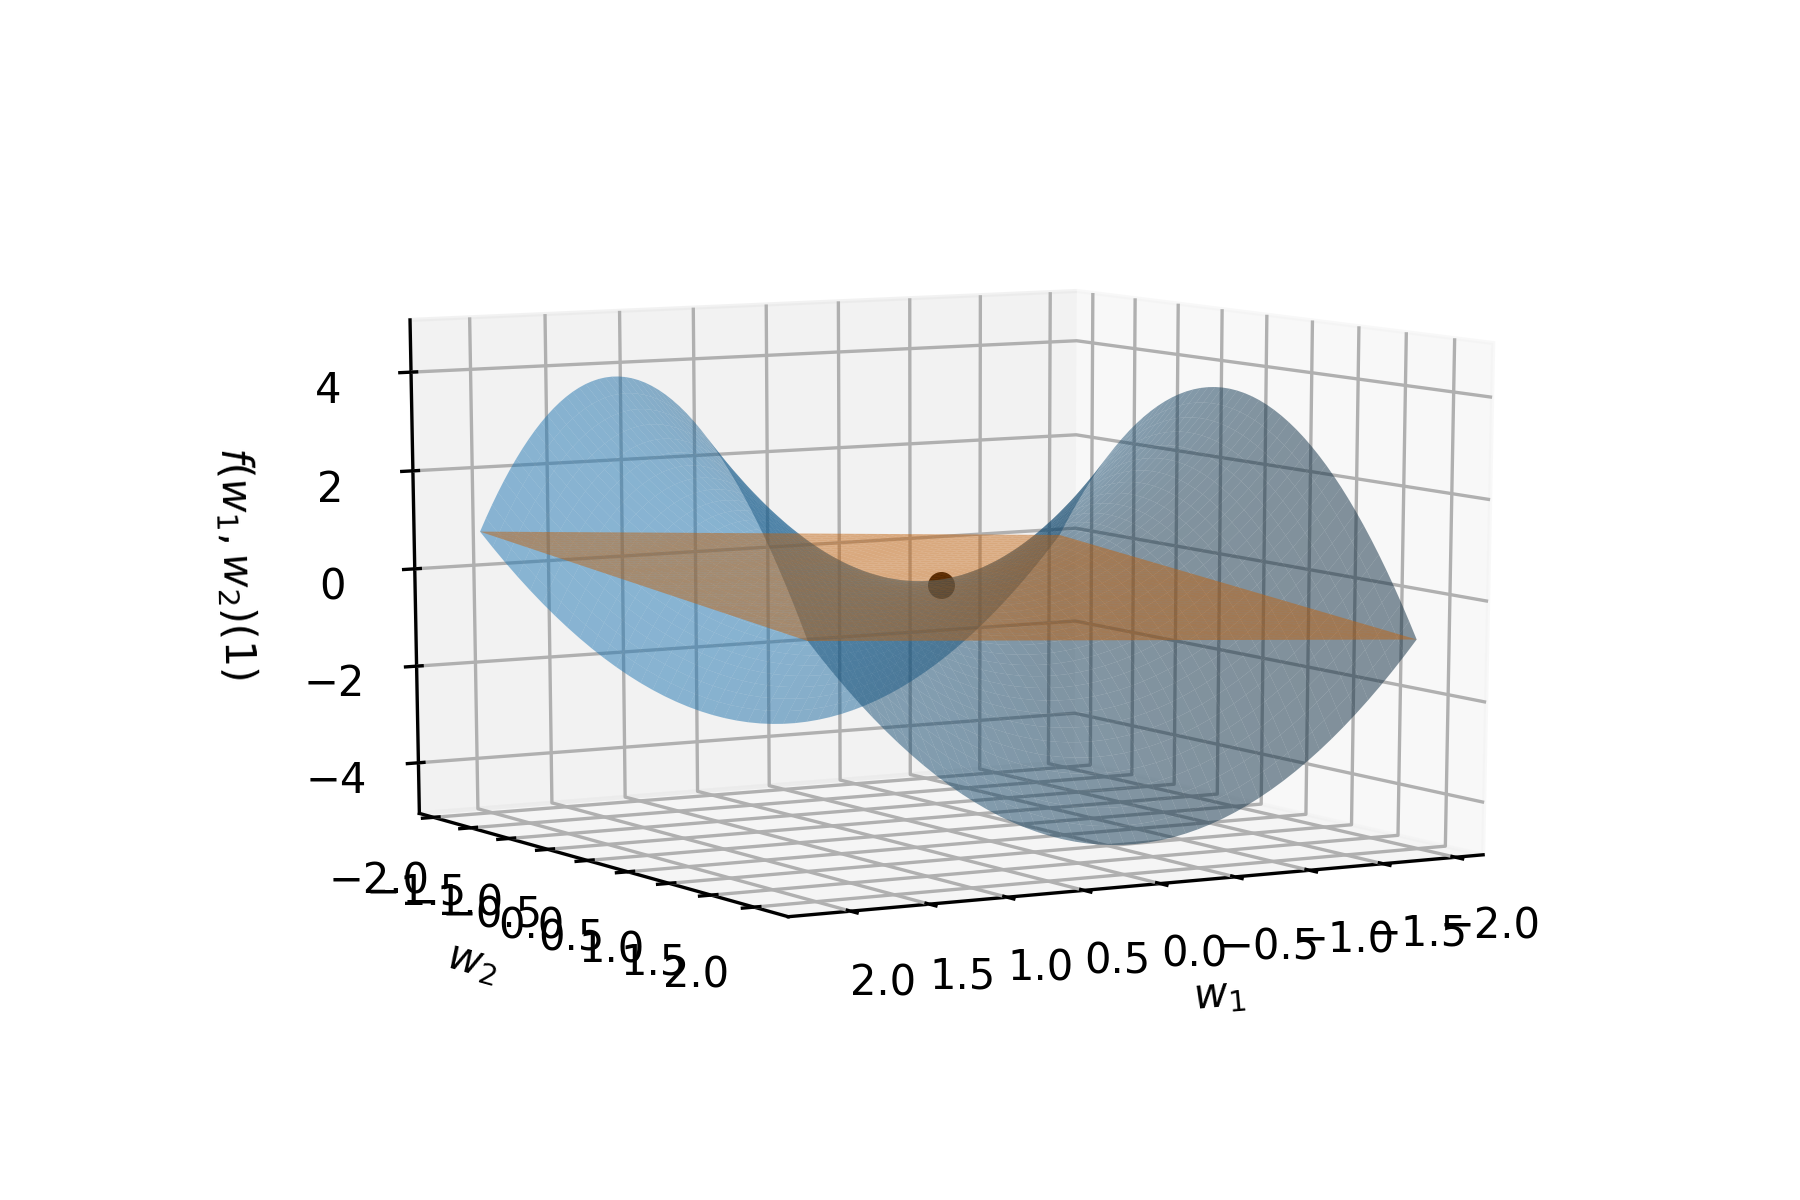
\includegraphics[width=.5\linewidth]{Imgs/Linearized_Model/visualize_linearized_0.1.png}}\hfill
    \subfloat[$\alpha = 10^1$]{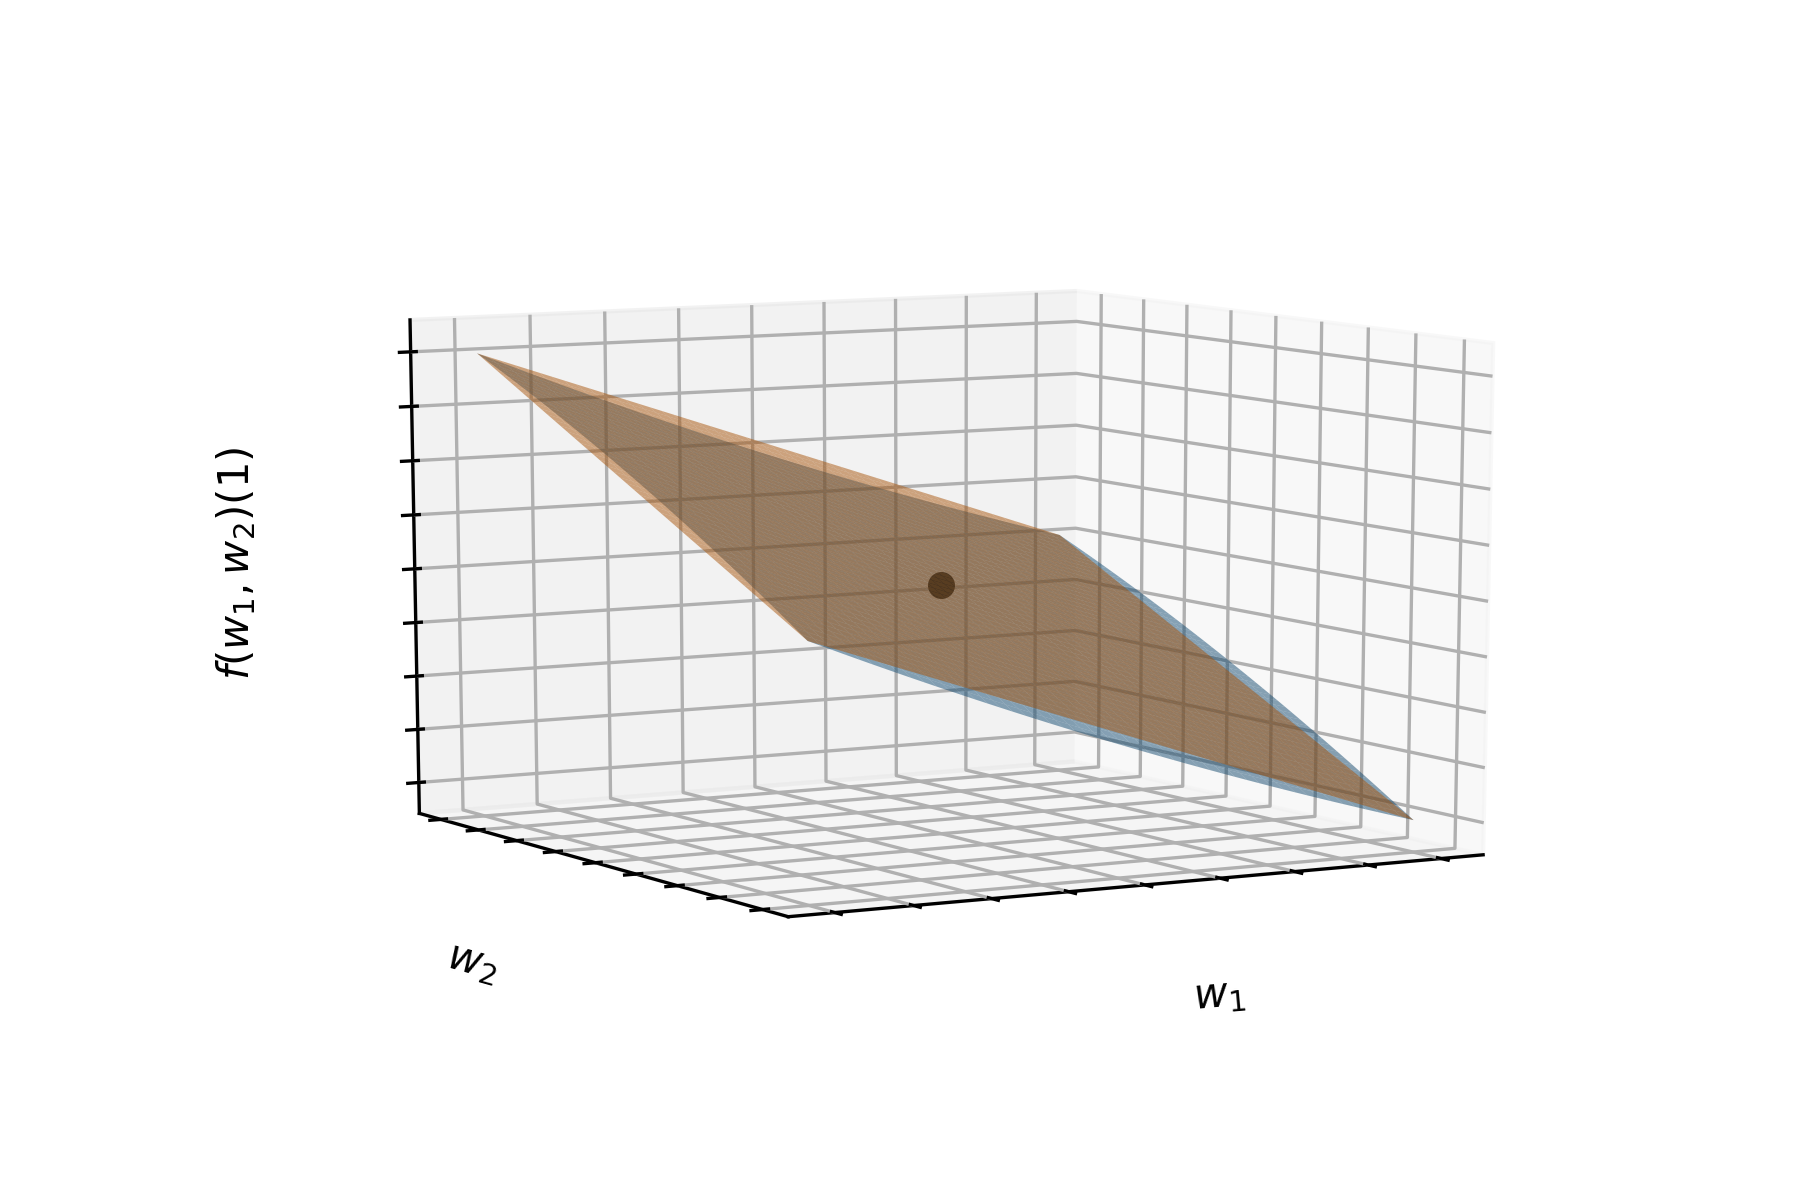
\includegraphics[width=.5\linewidth]{Imgs/Linearized_Model/visualize_linearized_10.png}}
    \caption{The linear regression model $f(\boldsymbol{w}, \boldsymbol{x})$ with one-dimensional input $\boldsymbol{x} = 1$ and weights $\boldsymbol{w} = (w_1, w_2)$ initialized at $\boldsymbol{w}_{\alpha}(0) = \alpha \mathbbm{1}$. The original linear regression model $f(w_1, w_2)(1)$ is plotted in blue, and the linearized model $\bar{f}(w_1, w_2)(1)$ is in orange.}\label{img:linearization}
\end{figure}

Now that we have given exact characterizations of the kernel and rich limits for the linear regression problem, we wish to empirically demonstrate the transition between the two limits. Our first demonstration aims to represent the relationship between the original model $f(\boldsymbol{w}, \boldsymbol{x}) = \sum_{i=1}^n (\boldsymbol{w}_{i,+}^2 - \boldsymbol{w}_{i,-}^2)\boldsymbol{x}_i$ and the linearized model $\bar{f}(\boldsymbol{w}, \boldsymbol{x}) = \langle \varphi_{\boldsymbol{w}_{\alpha}(0)}(\boldsymbol{x}), \boldsymbol{w} - \boldsymbol{w}_{\alpha}(0) \rangle = 2\alpha \langle \boldsymbol{x} , \boldsymbol{w}_+ - \boldsymbol{w}_-\rangle$ with initialization $\boldsymbol{w}_{\alpha}(0) = \alpha \mathbbm{1}$. In particular, we know from Section \ref{defkernelrich} that as $\alpha \rightarrow \infty$, the gradient flow $(\boldsymbol{w}_{\alpha}(t))_{t \geq 0}$ is identical to $(\boldsymbol{\bar{w}}_{\alpha}(t))_{t \geq 0}$ with $\boldsymbol{w}_{\alpha}(0) = \boldsymbol{\bar{w}}_{\alpha}(0) = \alpha \mathbbm{1}$. And so we should observe that for fixed $\boldsymbol{x} \in \mathcal{X}$, $f(\boldsymbol{w}, \boldsymbol{x})$ is approximately equal to $\bar{f}(\boldsymbol{w}, \boldsymbol{x})$ as a function of $\boldsymbol{w} \in \mathbb{R}^p$ around the initialization $\boldsymbol{w}_{\alpha}(0) = \alpha \mathbbm{1}$. Conversely, as $\alpha \rightarrow 0$ we should observe that for fixed $\boldsymbol{x}$, $f(\boldsymbol{w}, \boldsymbol{x})$ is differs substantially from $\bar{f}(\boldsymbol{w}, \boldsymbol{x})$ around $\boldsymbol{w}_{\alpha}(0) = \alpha \mathbbm{1}$.

Since $\boldsymbol{w}$ increases quickly in dimension as $n$ grows, we consider the case of $n =1$. That is, we have a linear regression model with a single slope coefficient $\beta_{\boldsymbol{w}} = \boldsymbol{w}_{+, 1}^2 - \boldsymbol{w}_{-, 1}^2$. For simplicity, let us define $w_1 := \boldsymbol{w}_{+, 1}$, $w_2 := \boldsymbol{w}_{-, 1}$, and so we can view $f$ as a neural network with a one-dimensional input $x$ and two weights $w_1, w_2$. For our demonstrations, we choose the input $x = 1$ to be fixed. And so we are interested in the functions $f(w_1, w_2)(1), \bar{f}(w_1, w_2)(1): \mathbb{R}^2 \rightarrow \mathbb{R}$ mapping from the parameter space to the network output.

In Figure \ref{img:linearization}, we plot each of $f(w_1, w_2)(1)$ and $\bar{f}(w_1, w_2)(1)$ on the square grid $[\alpha - 2, \alpha + 2] \times [\alpha - 2, \alpha + 2]$ for $\alpha = 10^{-1}, 10^1$. Notice that the initialization $\boldsymbol{w}_{\alpha}(0) = \alpha \mathbbm{1}$ is at the center of this grid, and the black point represents $f(w_1, w_2)(1)$ evaluated at its initialization, $(\boldsymbol{w}_{\alpha}(0), f(\boldsymbol{w}_{\alpha}(0))(1)) = (\alpha \mathbbm{1}, 0)$. For all $\alpha \in \mathbb{R}_{++}$, $f$ is equal to $\bar{f}$ at its initialization: $f(\boldsymbol{w}_{\alpha}(0))(1) = \bar{f}(\boldsymbol{w}_{\alpha}(0))(1)$. When $\alpha = 10^1$, we see that $|f(w_1, w_2)(1) - \bar{f}(w_1, w_2)(1) |$ is small for $\| (w_1, w_2) - \alpha \mathbbm{1} \|_2 > 0$, meaning $f$ is close to the affine model $\bar{f}$ around $\boldsymbol{w}_{\alpha}(0) = \alpha \mathbbm{1}$. On the other hand, when $\alpha = 10^{-1}$ we observe that $|f(w_1, w_2)(1) - \bar{f}(w_1, w_2)(1)|$ is large for $\| (w_1, w_2) - \alpha \mathbbm{1} \|_2 > 0$. That is, $f$ is highly nonlinear in $(w_1, w_2)$ about $\boldsymbol{w}_{\alpha}(0) = \alpha \mathbbm{1}$, and so is far from its linearization around $\boldsymbol{w}_{\alpha}(0)$, $\bar{f}$.

\begin{figure}[H]
\animategraphics[loop, controls, width=\textwidth]{10}{Imgs/Linearized_Model/GIF_imgs/visualize_linearized_}{0}{99}
\caption{The linear regression model $f(w_1, w_2)(1)$ (blue) and the corresponding linearized model $\bar{f}(w_1, w_2)(1)$ (orange) for initialization scale $10^{-1} \leq \alpha \leq 10^1$.}\label{gif:linearization}
\end{figure}

Letting the initialization scale $\alpha$ vary between $10^{-1}$ and $10^{1}$ in Figure \ref{gif:linearization}, we provide an even clearer representation of the relationship between the original model $f(w_1, w_2)(1)$ and the linearization of $f$ around $\boldsymbol{w}_{\alpha}(0) = \alpha \mathbbm{1}$, $\bar{f}(w_1, w_2)(1)$. %Once again, we take the grid of input weights to be the region $[\alpha - 2, \alpha + 2] \times [\alpha - 2, \alpha + 2]$ containing $\boldsymbol{w}_{\alpha}(0)$.

From our illustrations, it is evident that for $\alpha \ll 1$, the gradient flow on $L(h(\boldsymbol{w}))$ with initialization $\boldsymbol{w}_{\alpha}(0) = \alpha \mathbbm{1}$ would result in quite a different model than that resulting from the gradient flow on $L(\bar{h}(\boldsymbol{w}))$. But as $\alpha$ grows away from $0$, $h$ approaches $\bar{h}$ around $\boldsymbol{w}_{\alpha}(0)$ and the two gradient flow paths are nearly identical.


\subsection{The Neural Tangent Kernel}\label{visualizeNTK}

The next aspect of the kernel and rich limits that we wish to illustrate is the neural tangent kernel (NTK). Recall that in Section \ref{linregmodel} we derived the NTK corresponding to the linear regression model at $\boldsymbol{w}_{\alpha}(0)$ to be
\begin{align*}
K_{\boldsymbol{w}_{\alpha}(0)}(\boldsymbol{x}_1, \boldsymbol{x}_2) = 8\alpha^2 \langle \boldsymbol{x}_1, \boldsymbol{x}_2 \rangle \quad \boldsymbol{x}_1, \boldsymbol{x}_2 \in \mathcal{X},
\end{align*}
One will also recall our discussion in Section \ref{kernelmethod} that since $h(\boldsymbol{w}_{\alpha}(0)) = 0$ and $L$ is the mean-squared error, then in the limit $\alpha \rightarrow \infty$ the gradient flow on $L(h(\boldsymbol{w}))$ is equivalent to a kernel method with kernel $K_{\boldsymbol{w}_{\alpha}(0)}$. %Put differently, in the kernel limit we are looking for a function $f^{\star}$ in the fixed feature space given by $\varphi_{\boldsymbol{w}_{\alpha}(0)}(\boldsymbol{x})$ which is a global minimizer of $L$ \cite{wei2019regularization}.

\begin{figure}[H]
\centering
\subfloat[$\alpha = 10^{-1}$]{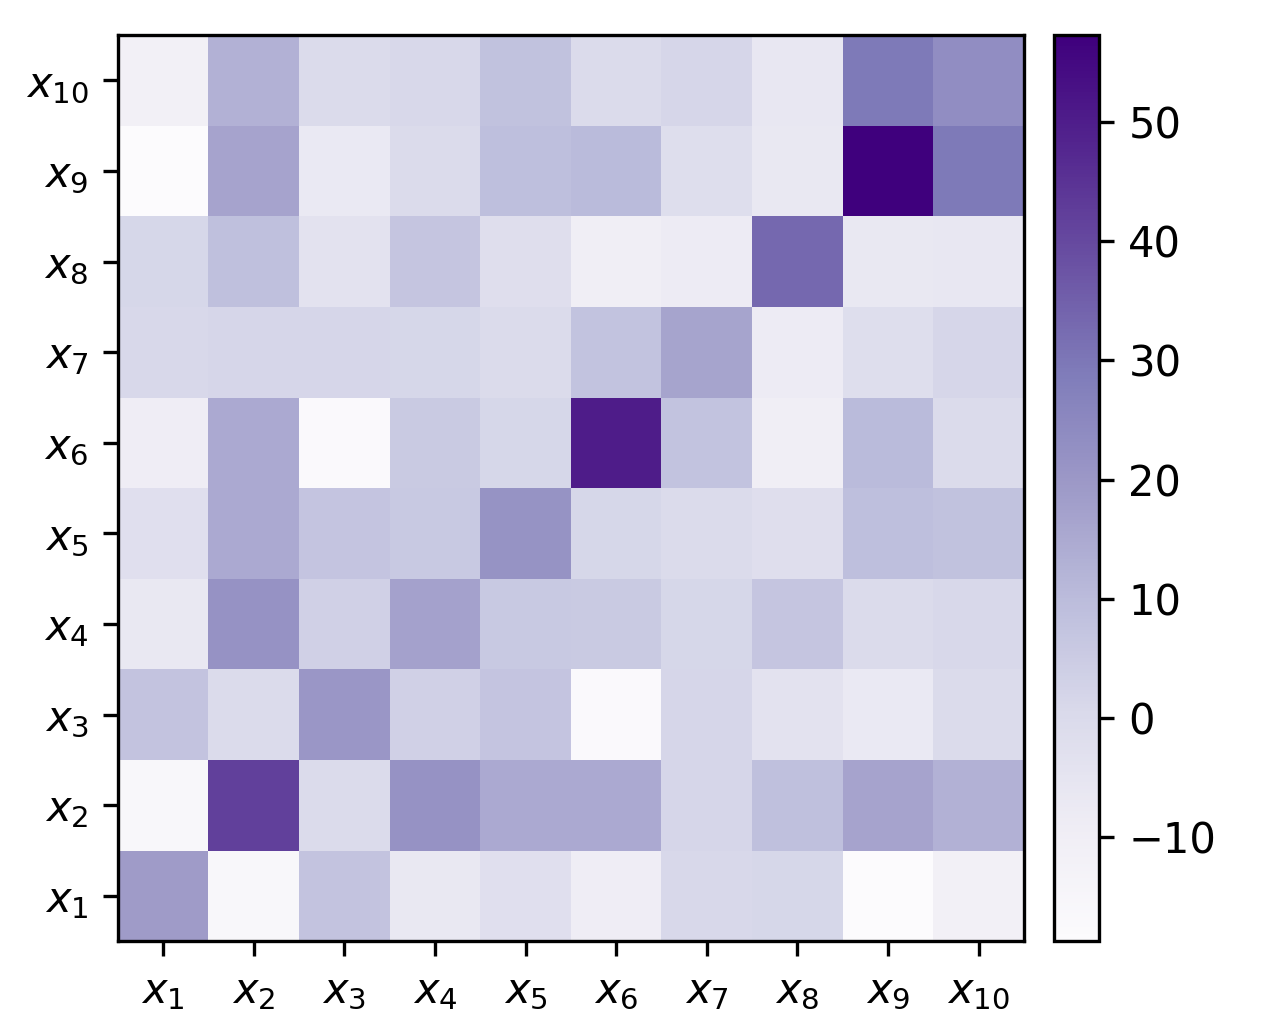
\includegraphics[width=.45\linewidth]{Imgs/NTK/NTK_0.1/NTK_0.1_change_total_cropped.png}}\hfill
\subfloat[$\alpha = 1$]{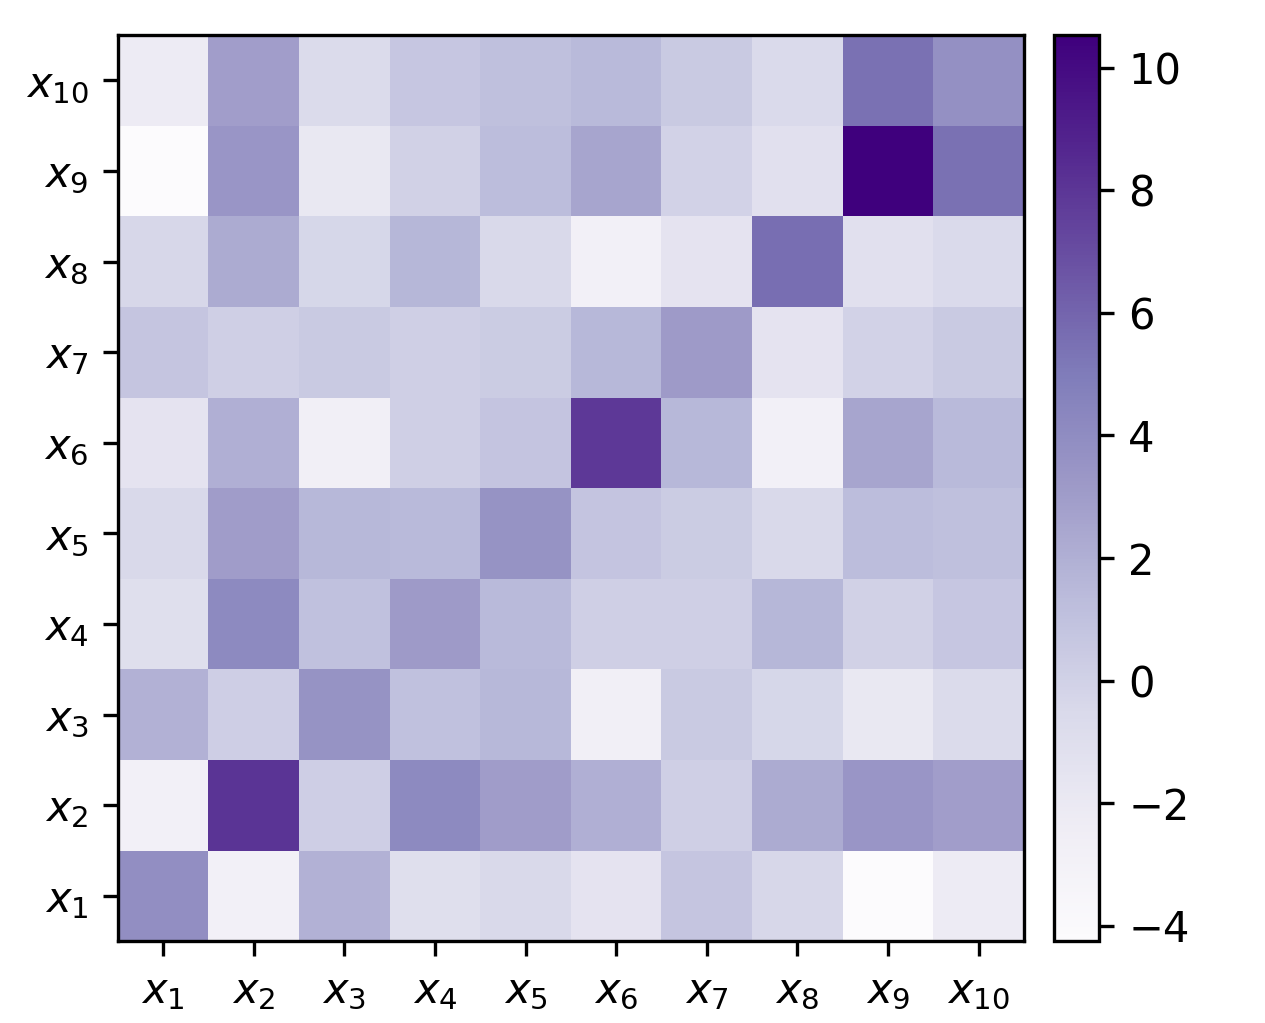
\includegraphics[width=.45\linewidth]{Imgs/NTK/NTK_1/NTK_1_change_total_cropped.png}}\par 
\subfloat[$\alpha = 10^{1}$]{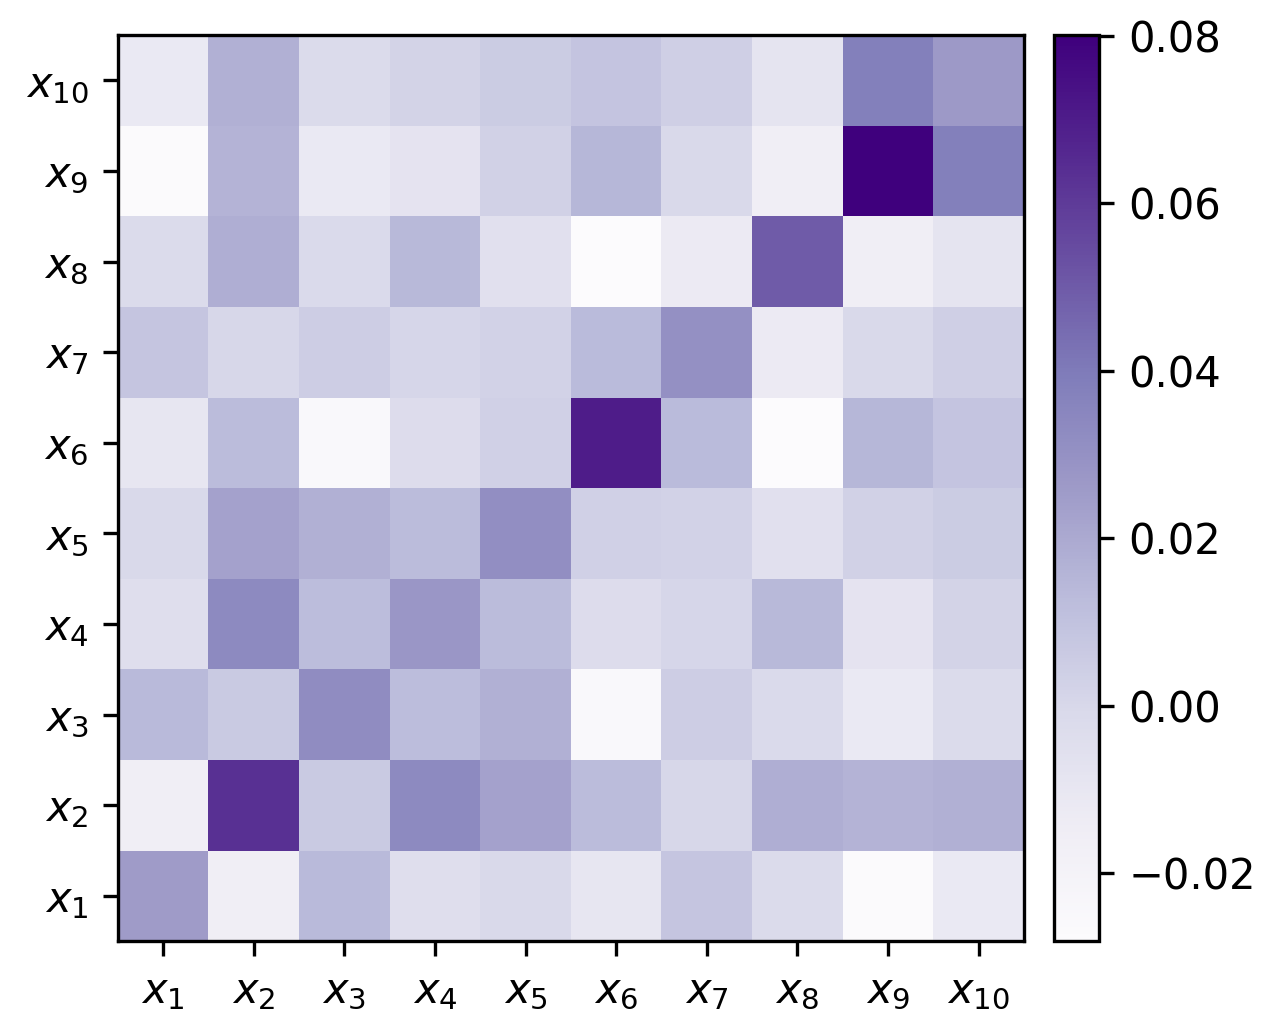
\includegraphics[width=.45\linewidth]{Imgs/NTK/NTK_10/NTK_10_change_total_cropped.png}}
\caption{The change in the neural tangent kernel (NTK) evaluated on the grid of $N= 10$ training points $\{ \boldsymbol{x}_i \}_{i=1}^{10}$ throughout training with gradient descent. For each of $\alpha = 10^{-1}, \ 1, \ 10^{1}$, we display the difference between the NTK at initialization $\boldsymbol{w}_{\alpha}(0)$ and at the end of training $\boldsymbol{w}_{\alpha}(t_{\text{end}})$.}\label{img:ntkchange}
\end{figure}

To summarize our theoretical discussion, we know that in the kernel limit, the neural tangent kernel $K_{\boldsymbol{w}_{\alpha}(t)}(\boldsymbol{x}_1, \boldsymbol{x}_2)$, $\boldsymbol{x}_1, \boldsymbol{x}_2 \in \mathcal{X}$ should remain equal to $K_{\boldsymbol{w}_{\alpha}(0)}(\boldsymbol{x}_1, \boldsymbol{x}_2)$ for all times $t \in \mathbb{R}_+$ in the gradient flow $(\boldsymbol{w}_{\alpha}(t))_{t \geq 0}, \ \boldsymbol{w}_{\alpha}(0) = \alpha \mathbbm{1}$ on $L(h(\boldsymbol{w}))$. Conversely, in the rich limit $\alpha \rightarrow 0$ we should observe that $K_{\boldsymbol{w}_{\alpha}(t)}(\boldsymbol{x}_1, \boldsymbol{x}_2)$ evolves greatly throughout the gradient flow dynamics.

In order to demonstrate that the neural tangent kernel does, in fact, behave in this way, we consider gradient descent on $L(h(\boldsymbol{w}))$. We once again start with $\boldsymbol{w}_{\alpha}(0) = \alpha \mathbbm{1}$, and we let $(\boldsymbol{w}_{\alpha}(t))_{t \in \mathbb{N} \cup \{ 0\}}$ be our gradient descent path. As we previously hinted at in Section \ref{preliminaries}, gradient descent can be viewed as a forward Euler discretization of the gradient flow dynamics with positive stepsize $\eta > 0$. Accordingly, the gradient descent update is given by $\boldsymbol{w}_{\alpha}(t) = \boldsymbol{w}_{\alpha}(t-1) - \eta \nabla_{\boldsymbol{w}} (L(h(\boldsymbol{w})))|_{\boldsymbol{w} = \boldsymbol{w}_{\alpha}(t-1)}$ for each $t \in \mathbb{N}$.

As for our training data, we consider $N=10$ points $\{ (\boldsymbol{x}_i, y_i) \}_{i=1}^N$ where each $\boldsymbol{x}_i \in \mathbb{R}^{n}$, $n = 20$ and $y_i \in \mathbb{R}$. As was done by Woodworth and colleagues in \cite{woodworth2020kernel}, we draw our input points according to $\boldsymbol{x}_i \overset{i.i.d.}{\sim} \mathcal{N}(\boldsymbol{0}, \mathbbm{I}_{n \times n})$. And to generate the corresponding set of response points, we compute $y_i = \langle \boldsymbol{x}_i, \boldsymbol{\beta} \rangle$, where $\boldsymbol{\beta}$ is generated according to the joint uniform distribution on $[-1, 1]^n$. Clearly, there is at least one vector, namely $\boldsymbol{\beta}_{\boldsymbol{w}} = \boldsymbol{\beta}$, such that $f = \langle \boldsymbol{\beta}_{\boldsymbol{w}}, \boldsymbol{x} \rangle, \ \boldsymbol{x} \in \mathcal{X}$ is a global minimizer of the loss $L$.

Since our goal is to study the NTK in the kernel and rich regimes, we consider the gradient descent paths corresponding to initialization scales $\alpha = 10^{-1}, \ 1, \ 10^{1}$. To ensure that no one gradient descent path achieves smaller loss than the others, we stop training for each path once $L(h(\boldsymbol{w}_{\alpha}(t))) < 10^{-4}$. As one could likely predict, the challenge then becomes choosing a stepsize $\eta > 0$ such that $L(h(\boldsymbol{w}_{\alpha}(t)))$ converges within $10^{-4}$ of the global minimum. In particular, we would like to choose $\eta$ to be as small as possible while still achieving the desired convergence within a maximum of $10^4$ training epochs. Note that within each epoch, we use batch size $32$ to calculate the gradients and perform the reciprocal update steps. A small learning rate $\eta$ is preferable because in the limit $\eta \rightarrow 0$, the gradient descent with stepsize $\eta$ reproduces the gradient flow dynamics. In the table below, we summarize our choice of stepsize $\eta$ for each gradient descent path:
\begin{table}[H]
\centering
\begin{tabular}{ c|c|c } 
$\alpha$ & $\eta$ & Number of Epochs to Convergence \\
\hline
$10^{-1}$ & $10^{-2}$ & $1001$ \\ 
$1$ & $10^{-3}$ & $757$ \\
$10^1$ & $10^{-4}$ & $77$
\end{tabular}
\caption{}\label{table:NTK}
\end{table}

Evidently, no single stepsize $\eta > 0$ works for all initialization scales. One aspect of our experiment that is potentially problematic is that the stepsize corresponding to the gradient descent path $\alpha = 10^{-1}$ is quite large. Therefore, it may be the case that the gradient descent path $(\boldsymbol{w}_{\alpha = 10^{-1}}(t))_{t \in \mathbb{N} \cup \{ 0 \}}$ is quite far from the corresponding gradient flow dynamics $(\boldsymbol{w}_{\alpha = 10^{-1}}(t))_{t\geq 0}$. With more computational power, it may be possible to achieve convergence with a smaller stepsize by increasing the maximum number of training epochs to be greater than $10^4$.

Before the first training epoch and after the final epoch we evaluate the neural tangent kernel $K_{\boldsymbol{w}_{\alpha}(t)}$ on the $10 \times 10$ grid of training points $\{ \boldsymbol{x}_i \}_{i=1}^N$. We do the same every ten training epochs in order to understand how the neural tangent kernel evolves throughout training.

In Figure \ref{img:ntkchange}, we report the overall change in the NTK
\begin{align*}
   K_{\boldsymbol{w}_{\alpha}(t_{\text{end}})}(\boldsymbol{x}_i, \boldsymbol{x}_j) -  K_{\boldsymbol{w}_{\alpha}(0)}(\boldsymbol{x}_i, \boldsymbol{x}_j)
\end{align*}
on $\{ \boldsymbol{x}_i \}_{i=1}^N$ for the gradient descent paths with initialization scales $\alpha = 10^{-1}, \ 1, \ 10^1$. Here, $t_{\text{end}}$ denotes the final epoch of gradient descent as indicated in Table \ref{table:NTK}. Noticeably, for the large initialization scale $\alpha = 10^1$, the neural tangent kernel evaluated on the training grid changes very little from the beginning to the end of gradient descent. This empirically verifies our previous remarks about how we would expect the NTK to behave in the kernel regime, since in the kernel limit we have $K_{\boldsymbol{w}_{\alpha}(t)} = K_{\boldsymbol{w}_{\alpha}(0)}$ for all times $t \in \mathbb{R}_+$. Conversely, for the small initialization scale $\alpha = 10^{-1}$, we observe that the NTK varies greatly from the beginning to the end of training. That is, $K_{\boldsymbol{w}_{\alpha}(t_{\text{end}})}$ is very different from $K_{\boldsymbol{w}_{\alpha}(0)}$. Once again, this is how we would expect the NTK to evolve in the rich regime since the feature space determined by $\varphi_{\boldsymbol{w}_{\alpha}(t)}(\boldsymbol{x}) = \nabla_{\boldsymbol{w}}f(\boldsymbol{w}, \boldsymbol{x})|_{\boldsymbol{w} = \boldsymbol{w}_{\alpha}(t)}$ is not fixed in time $t \in \mathbb{R}_+$ in the rich limit as it is in the kernel limit. From our experiment, we also see the interpolation between the kernel and rich regimes. At $\alpha = 1$, we discern that that the NTK exhibits behavior between the kernel and rich regimes.

Although Figure \ref{img:ntkchange} certainly does portray how the neural tangent kernel changes from the beginning to the end of training, it does not fully capture how it evolves throughout training. To better understand the continuous time change of the NTK, we plot $K_{\boldsymbol{w}_{\alpha}(t)}$ on $\{ \boldsymbol{x}_i \}_{i=1}^N$ evaluated at every 10 epochs of gradient descent for the paths corresponding to $\alpha = 10^{-1}, \ 1$. We fix the scale of each plot Figure \ref{gif:ntk1} and Figure \ref{gif:ntk2} at $t = 0$ so that it does not automatically adjust at each evaluation of the NTK. Just as we would expect, the NTK corresponding to $\alpha = 10^{-1}$ experiences large relative changes, even at the end of training when $f(\boldsymbol{w}_{\alpha}(t), \boldsymbol{x})$ is close to a global minimum of the loss $L$. This is not the case for the gradient descent path corresponding to initialization scale $\alpha = 1$; in fact, it may appear as if the NTK does not change whatsoever. From Figure \ref{img:ntkchange} we know that this is not the case. Rather, for $\alpha = 1$ the changes in the NTK $K_{\boldsymbol{w}_{\alpha}(t)}$ are small relative to its scale at $\boldsymbol{w}_{\alpha}(0)$.

\begin{figure}[H]
\animategraphics[loop, controls, width=\textwidth]{10}{Imgs/NTK/NTK_0.1/GIF_imgs/linearized_NTK_0.1_}{0}{100}
\caption{The neural tangent kernel (NTK) evaluated on the grid of training points $\{ \boldsymbol{x}_i \}_{i=1}^N$ for every 10 epochs of gradient descent with initialization $\boldsymbol{w}_{\alpha = 10^{-1}}(0) = 10^{-1}\mathbbm{1}$.}\label{gif:ntk1}
\end{figure}

\newpage

\vspace*{\fill}
\begin{figure}[H]
\animategraphics[loop, controls, width=\textwidth]{10}{Imgs/NTK/NTK_1/GIF_imgs/linearized_NTK_1_}{0}{75}
\caption{The neural tangent kernel (NTK) evaluated on the grid of training points $\{ \boldsymbol{x}_i \}_{i=1}^N$ for every 10 epochs of gradient descent with initialization $\boldsymbol{w}_{\alpha = 1}(0) = \mathbbm{1}$.}\label{gif:ntk2}
\end{figure}
\vspace*{\fill}

\newpage

\subsection{The Model Weights}

\begin{figure}[H]
    \centering
    \subfloat[]{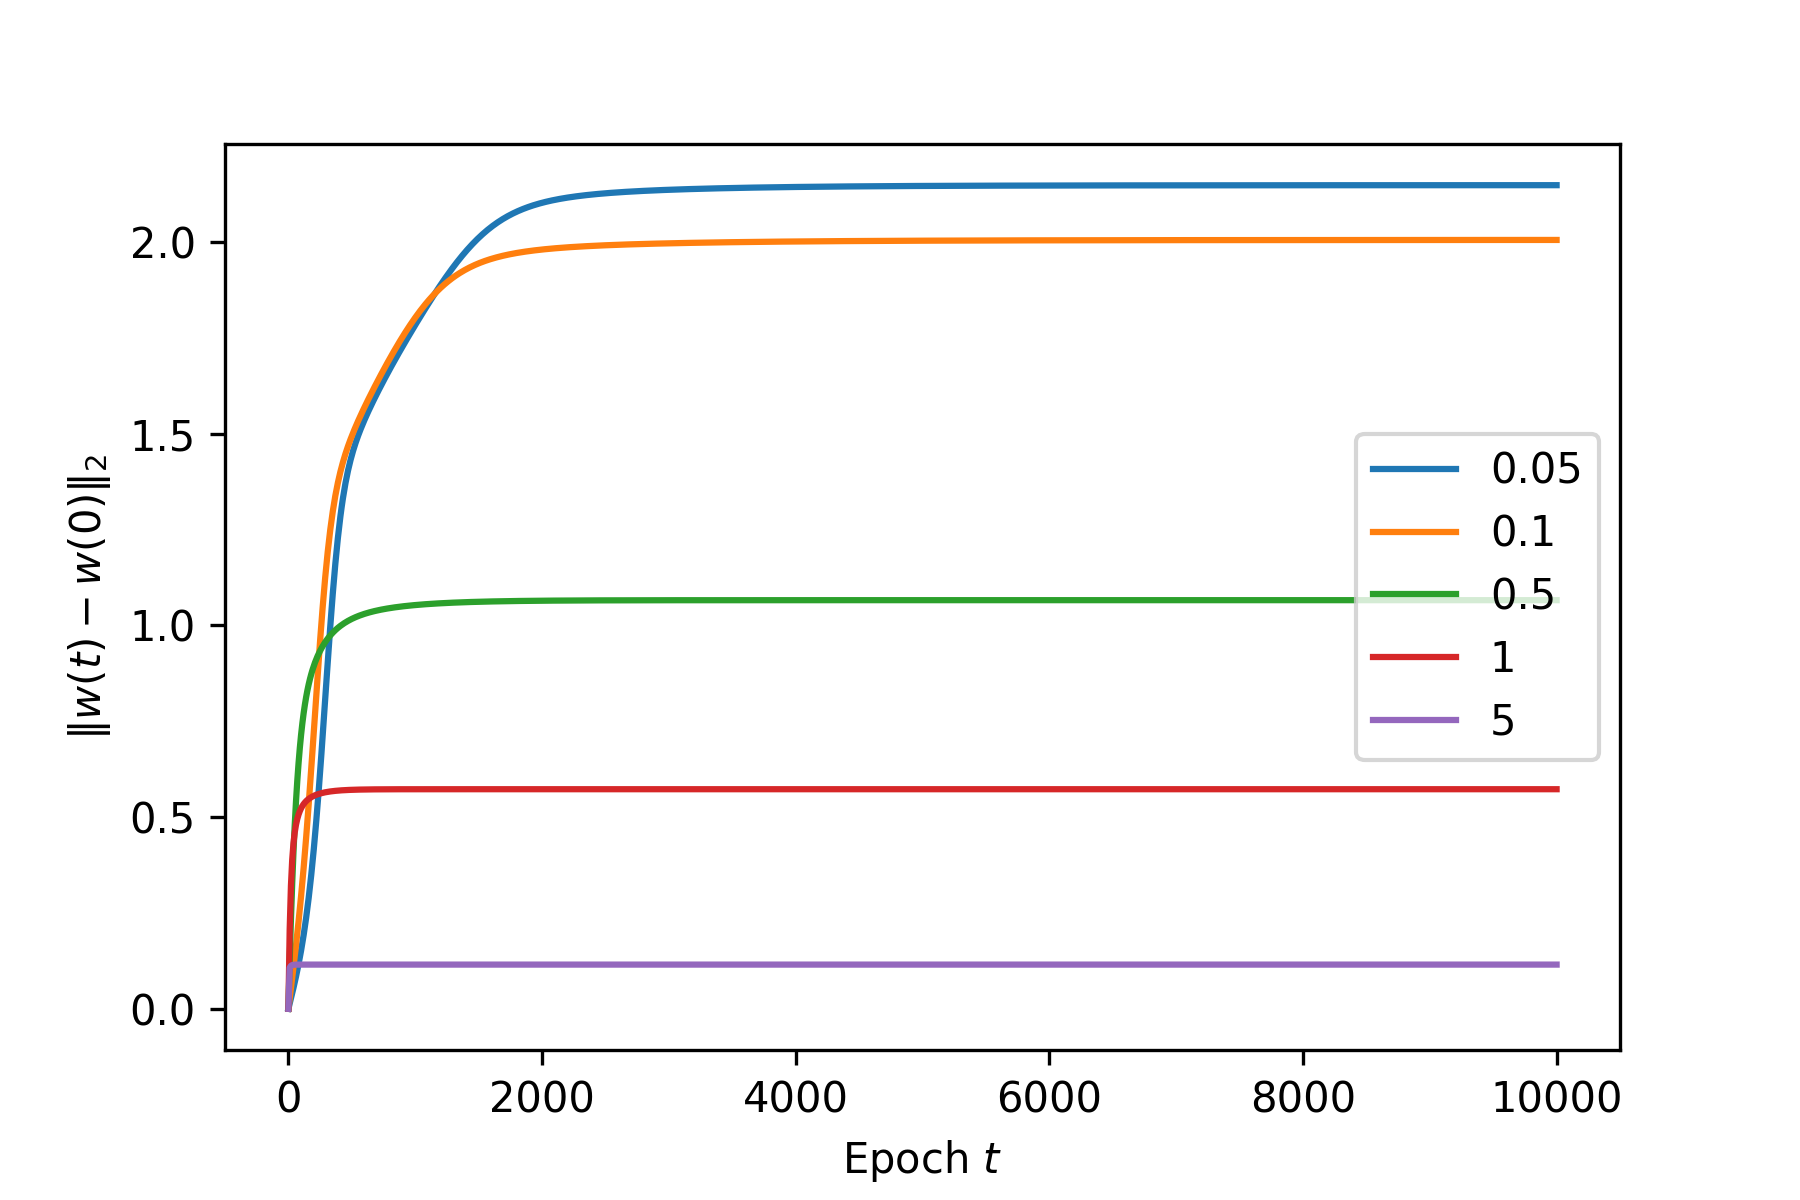
\includegraphics[width=.5\linewidth]{Imgs/Weights/visualize_change.png}\label{fig:weights:change}}\hfill
    \subfloat[]{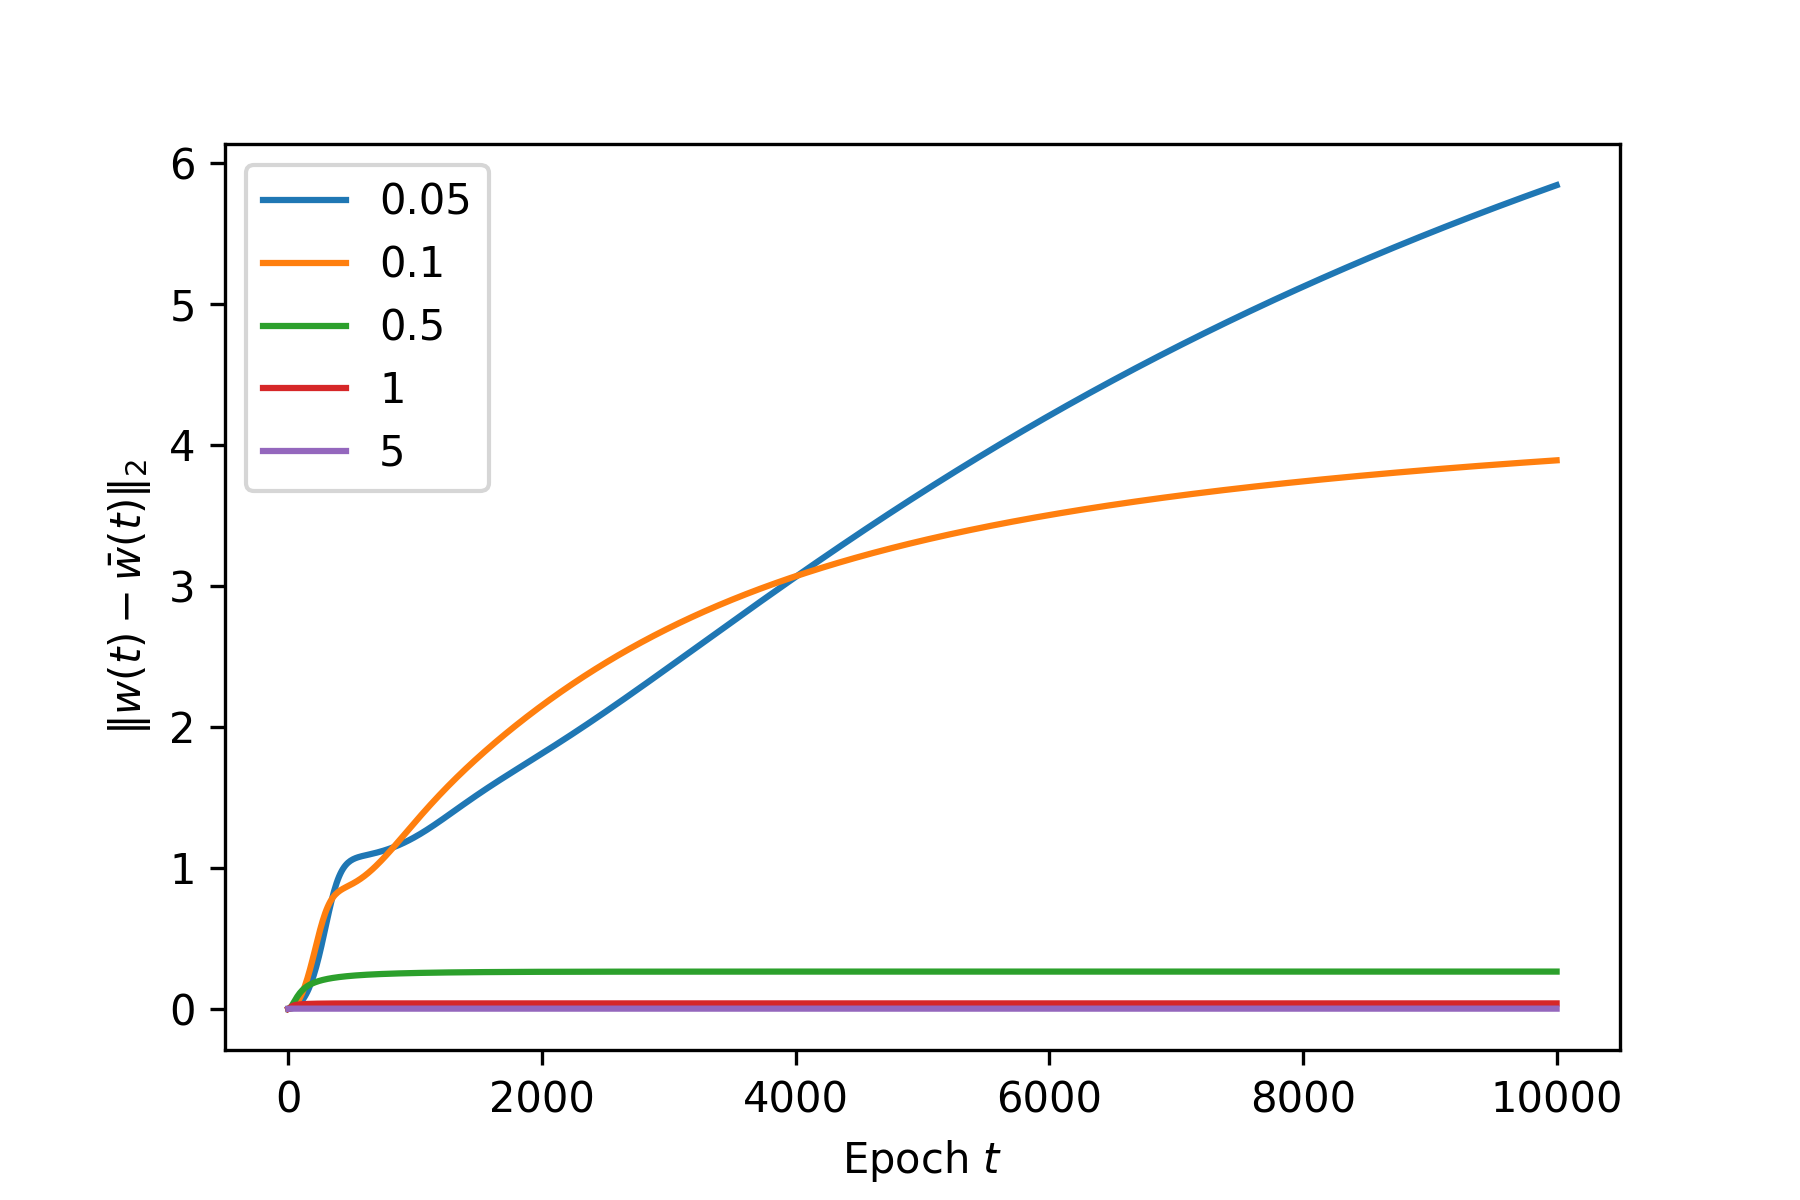
\includegraphics[width=.5\linewidth]{Imgs/Weights/visualize_weights.png}\label{fig:weights:diff}}
    \caption{(a) The $\ell^2$ distance between the weights of the model at epoch $t$ of gradient descent, $\boldsymbol{w}_{\alpha}(t)$, and at initialization $\boldsymbol{w}_{\alpha}(0) = \alpha \mathbbm{1}$. (b) The $\ell^2$ distance between the weights of the model $h$, $\boldsymbol{w}_{\alpha}(t)$, and those of the linearized model $\bar{h}$, $\boldsymbol{\bar{w}}_{\alpha}(t)$, at epoch $t$ of gradient descent. The initialization scale of each gradient descent path is indicated by the line color as reported in the plot legends.}\label{fig:weights}
\end{figure}

For our final demonstration of the kernel and rich limits in the linear regression problem, we consider how the weights of the model themselves $\boldsymbol{w}_{\alpha}(t)$ evolve throughout the gradient flow dynamics on $L(h(\boldsymbol{w}))$. From the results of Theorem \ref{Chizatthm2.2}, we know that in the kernel limit $\alpha \rightarrow \infty$ it holds that $\| \boldsymbol{w}_{\alpha}(t) - \boldsymbol{w}_{\alpha}(0) \|_2 \rightarrow 0$ as well as $\| \boldsymbol{w}_{\alpha}(t) - \boldsymbol{\bar{w}}_{\alpha}(t) \|_2 \rightarrow 0$ for each $t \in \mathbb{R}_+$. The first result tells us that for all times, the gradient flow path is asymptotically fixed at its initialization in the kernel limit. The second statement tells us that in the kernel limit, gradient flow on the original objective $L(h(\boldsymbol{w}))$ is equivalent to the gradient flow on $L(\bar{h}(\boldsymbol{w}))$. Using a similar setup to that in Section \ref{visualizeNTK}, we exhibit empirically that each of these two limits hold.


Just as in Section \ref{visualizeNTK}, we consider a training dataset of $N = 10$ points $\{(\boldsymbol{x}_i, y_i) \}_{i=1}^N$ with each $\boldsymbol{x}_i \in \mathbb{R}^n$, $n=20$ and $y_i \in \mathbb{R}$. The specifics of how we generate these $(\boldsymbol{x}_i, y_i)$ are exactly the same as in Section \ref{visualizeNTK}. Similar to our experiment for the neural tangent kernel, we once again consider the gradient descent with initialization $\boldsymbol{w}_{\alpha}(0) = \alpha \mathbbm{1}$ , denoted $(\boldsymbol{w}_{\alpha}(t))_{t \in \mathbb{N} \cup \{ 0\}}$, as a discretization of the gradient flow dynamics. Here, we specifically look at the gradient descent paths corresponding to intialization scales $\alpha \in \{ 5\times10^{-2}, 10^{-1}, 5 \times 10^{-1}, 1, 5\}$. Unlike in the previous experiment, though, we fix a stepsize $\eta = 10^{-3}$ for each $\alpha$ and do not stop training early once $L(h(\boldsymbol{w}_{\alpha}(t))) < 10^{-4}$. Rather, we run each gradient descent path for a total of $10^4$ epochs. The reason for this is that we would like to compare $\boldsymbol{w}_{\alpha}(t)$ for these various $\alpha$, which we cannot do if the stepsize varies along with $\alpha$. And once again, we use batch size $32$ to compute the gradient and perform the corresponding updates within each epoch.

In order to demonstrate the first limit, $\| \boldsymbol{w}_{\alpha}(t) - \boldsymbol{w}_{\alpha}(0) \|_2 \rightarrow 0$ as $\alpha \rightarrow \infty$, we store the network weights $\boldsymbol{w}_{\alpha}(t)$ both at the beginning of training $\boldsymbol{w}_{\alpha}(0) = \alpha \mathbbm{1}$ as well as after every 10 epochs of gradient descent. In Figure \ref{fig:weights:change}, we display the $\ell^2$ distance of $\boldsymbol{w}_{\alpha}(t)$ from the initialization $\boldsymbol{w}_{\alpha}(0)$ as a function of $t \in \mathbb{R}_+$. Just as we would expect under the aforementioned theory, the gradient descent path remains close to $\boldsymbol{w}_{\alpha}(0) = \alpha \mathbbm{1}$ whenever $\alpha$ is large. However, we do observe that the convergence of $\boldsymbol{w}_{\alpha}(t)$ to $\boldsymbol{w}_{\alpha}(0)$ is the most rapid for $t \in \mathbb{R}_+$ small. For the very large initialization scale $\alpha = 5$, we observe that $\boldsymbol{w}_{\alpha}(t)$ barely deviates from its initialization. On the opposite end of the paradigm, for $\alpha = 10^{-1}, \ 5 \times 10^{-2}$ we observe large changes in $\boldsymbol{w}_{\alpha}(t)$ throughout training. As we have previously elucidated, this active training is synonymous with the rich limit $\alpha \rightarrow 0$.

Furthermore, we are interested in the relationship between the gradient flow on $L(h(\boldsymbol{w}))$ and that on $L(\bar{h}(\boldsymbol{w}))$ in the kernel and rich limits. Since we have already computed $(\boldsymbol{w}_{\alpha}(t))_{t \geq 0}$, then it remains to calculate $(\boldsymbol{\bar{w}}_{\alpha}(t))_{t \in \mathbb{N} \cup \{ 0\}}$, the gradient descent path on the linearized objective function $L(\bar{h}(\boldsymbol{w}))$ with initialization $\boldsymbol{\bar{w}}(0) = \alpha \mathbbm{1}$. Just as we did for the original objective, we run gradient descent for $10^4$ total training epochs with batch size $32$ and stepsize $\eta = 10^{-3}$ . Likewise, we store the weights $\boldsymbol{\bar{w}}_{\alpha}(t)$ at the beginning of training and following every 10 gradient descent epochs. In Figure \ref{fig:weights:diff}, we report the $\ell^2$ distance between the gradient descent paths $\boldsymbol{w}_{\alpha}(t)$ and $\boldsymbol{\bar{w}}_{\alpha}(t)$ as a function of $t$. For large initialization scales $\alpha = 1, \ 5$, it is evident that $\boldsymbol{w}_{\alpha}(t)$ and $\boldsymbol{\bar{w}}_{\alpha}(t)$ are close, especially for small times $t \in \mathbb{R}_+$. This supports the assertion that the gradient flow on $L(h(\boldsymbol{w}))$ is equivalent to that on the linearized objective $L(\bar{h}(\boldsymbol{w}))$ in the kernel limit $\alpha \rightarrow \infty$. On the contrary, for $\alpha = 5 \times 10^{-2}, 10^{-1}$ small, we see that $\| \boldsymbol{w}_{\alpha}(t) - \boldsymbol{\bar{w}}_{\alpha}(t) \|_2$ increases substantially throughout training. This suggests that gradient flow on the original objective $L(h(\boldsymbol{w}))$ is very different from that on the linearized objective $L(\bar{h}(\boldsymbol{w}))$ in the rich limit $\alpha \rightarrow 0$.

\section{Rich Training and Sparse Generalization}\label{richgeneralization}

Thus far, we have provided theoretical characterizations of the kernel and rich limits for neural network training and have demonstrated that these limits do, in fact, hold for the linear regression model considered in \cite{woodworth2020kernel}. What has been notably absent from our discussion, though, is why the distinction between kernel and rich training is meaningful. That is, why should one be conscious about whether they are training their neural network near the kernel limit or near the rich limit? 

To address this question, we must study the implicit biases of networks trained in the kernel and rich limits. One will recall that in Section \ref{richkerneltheory} we derived the explicit kernel and rich limits for the linear regression model from \cite{woodworth2020kernel}. In the kernel limit gradient flow implements the minimum $\ell^2$ norm solution whereas rich limit implements the minimum $\ell^1$ norm solution. As Woodworth and colleagues point out, this result suggests benefits to training in the rich regime when one suspects that there is sparsity in the underlying distribution of data. This association of the rich limit with implicit $\ell^1$ regularization does not appear to be limited to the linear regression model, though. In Section \ref{sparselogistic}, we provide experimental results which suggest that for a sparse binary classification problem, the rich limit imposes $\ell^1$ regularization in the parameter space.

\subsection{The Sparse Linear Regression Problem}\label{sparselinear}

To begin our examination of the implicit biases corresponding to the kernel and rich limits, we will look at the linear regression problem studied in Section \ref{linregmodel}. In particular, we know that for the model
\begin{align*}
    h(\boldsymbol{w}) = f(\boldsymbol{w}, \boldsymbol{x}) = \sum_{i=1}^n(\boldsymbol{w}_{+, i}^2 - \boldsymbol{w}_{-, i}^2)\boldsymbol{x}_i = \langle \boldsymbol{\beta}_{\boldsymbol{w}}, \boldsymbol{x} \rangle \qquad \boldsymbol{\beta}_{\boldsymbol{w}} = \boldsymbol{w}_+^2 -\boldsymbol{w}_-^2
\end{align*}
with loss function $L$ the mean-squared error, then gradient flow on the objective $L(h(\boldsymbol{w}))$, denoted\\ $(\boldsymbol{w}_{\alpha}(t))_{t \geq 0}$, with intialization $\boldsymbol{w}_{\alpha}(0) = \alpha \mathbbm{1}$ satisfies
\begin{align*}
    \lim_{t \to \infty}\lim_{\alpha \to \infty} \boldsymbol{\beta}_{\boldsymbol{w}_{\alpha}(t)} = \argmin_{\boldsymbol{\beta} \in \mathbb{R}^n}  \| \boldsymbol{\beta} \|_2, \qquad 
    \lim_{t \to \infty}\lim_{\alpha \to 0} \boldsymbol{\beta}_{\boldsymbol{w}_{\alpha}(t)} = \argmin_{\boldsymbol{\beta} \in \mathbb{R}^n}  \| \boldsymbol{\beta} \|_1.
\end{align*}

This result suggests that training in the rich regime will outperform training in the kernel regime when there is sparsity in the underlying distribution $\rho$ from which the data $(\boldsymbol{x}_i, y_i)$ is drawn. When we say \enquote{outperform,} note that we are not referring to how well the model fits the training data. The predictors implemented by gradient flow in both the kernel and rich limits interpolate the training data. Instead, we are referring to the generalization of the model on unseen data. If $(\boldsymbol{x}, y) \sim \rho$, then we can quantify how well a function $f \in \mathcal{F}$ generalizes according to
\begin{align}\label{poprisk}
\mathbb{E}_{(\boldsymbol{x}, y) \sim \rho}[(y - f(\boldsymbol{x}))^2],
\end{align}
which is the population risk corresponding to the square loss. For the case of linear regression, when we say that the distribution $\rho$ is \enquote{sparse,} we mean that a sparse predictor $\boldsymbol{\beta} \in \mathbb{R}^n$ minimizes the population risk.

In order to demonstrate this desirable property of training near the rich limit for the linear regression model, we consider the following problem that is formulated by Woodworth and colleagues. Suppose we have a training dataset of $N$ points $\{(\boldsymbol{x}_i, y_i)\}_{i=1}^N$, where each $\boldsymbol{x}_i \in \mathbb{R}^n$, $y_i \in \mathbb{R}$ for $n = 250$. The input data $\boldsymbol{x}_i$ is distributed according to $\mathcal{N}(\boldsymbol{0},\mathbbm{I}_{n \times n})$ and the corresponding output data is distributed according to $\mathcal{N}(\langle \boldsymbol{\beta}_{\boldsymbol{w}}, \boldsymbol{x}_i \rangle, \sigma^2)$ where $(\boldsymbol{\beta}_{\boldsymbol{w}})_i = 1/\sqrt{5}$ for $1 \leq i \leq 5$ and $(\boldsymbol{\beta}_{\boldsymbol{w}})_i = 0$ otherwise. Here, $\sigma^2 = 10^{-2}$ is a constant which determines the amount of noise in the output data. One should observe that the data we consider is very high-dimensional, and yet the population risk is minimized by $\boldsymbol{\beta} = \boldsymbol{\beta}_{\boldsymbol{w}}$, which has only five nonzero coordinates.

Just as in Section \ref{summarizekernel}, we approximate the gradient flow dynamics on $L(h(\boldsymbol{w}))$, $(\boldsymbol{w}_{\alpha}(t))_{t \geq 0}$, using the corresponding gradient descent path, $(\boldsymbol{w}_{\alpha}(t))_{t \in \mathbb{N} \cup \{ 0\}}$, with small stepsize $\eta = 3 \times 10^{-4}$. To ensure that we are fairly comparing the solution vectors $\boldsymbol{w}_{\alpha}(t_{\text{end}})$, we stop training once $L(h(\boldsymbol{w}_{\alpha}(t))) < 10^{-4}$. Since it might be the case, as we encountered in Section \ref{visualizeNTK}, that gradient descent converges very slowly to a global minimum of the objective function, we stop training after a maximum of $10^4$ epochs. Just as before, we use batch size 32 to compute the gradients and update the parameters.

\begin{figure}[H]
    \centering
    \subfloat[]{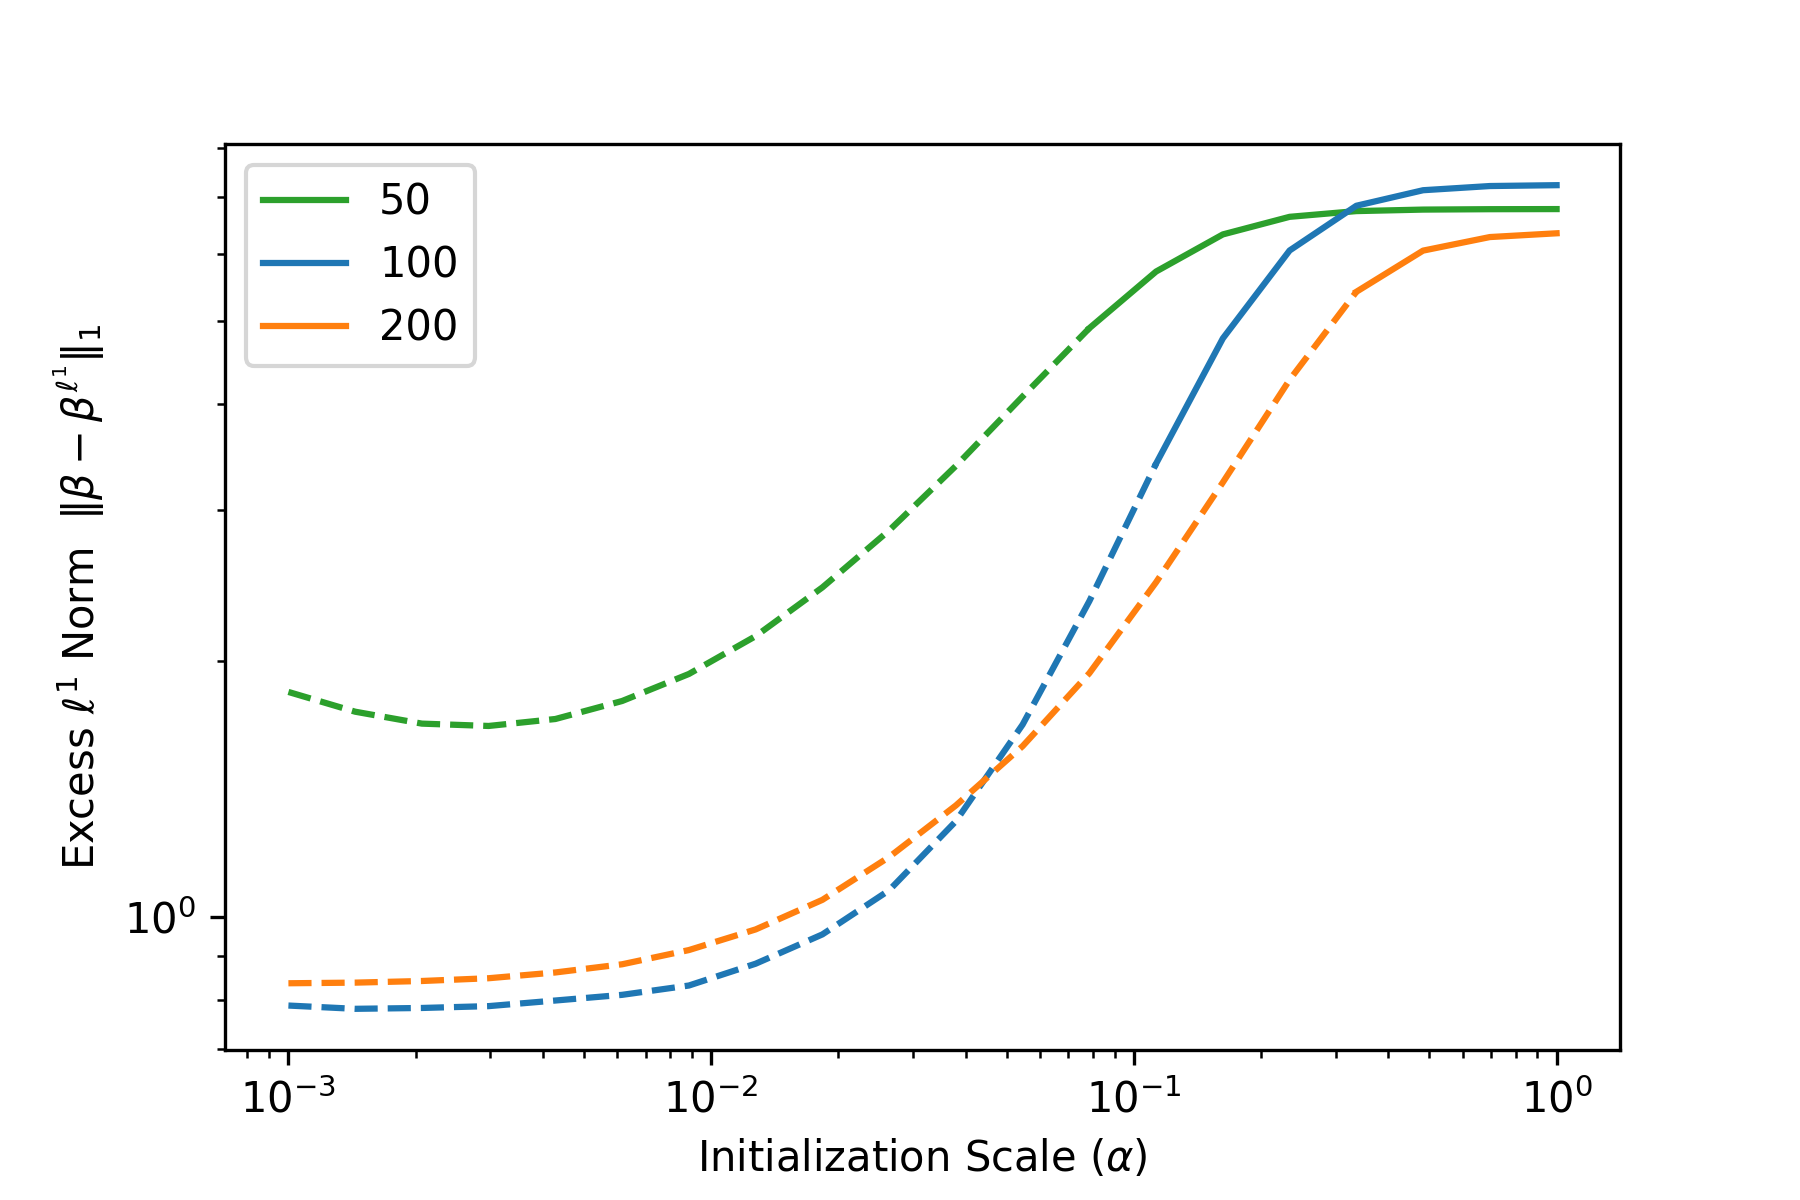
\includegraphics[width=.5\linewidth]{Imgs/Sparse Linear Regression/excess_l1_log_all.png}\label{fig:excessl1error}}\hfill
    \subfloat[]{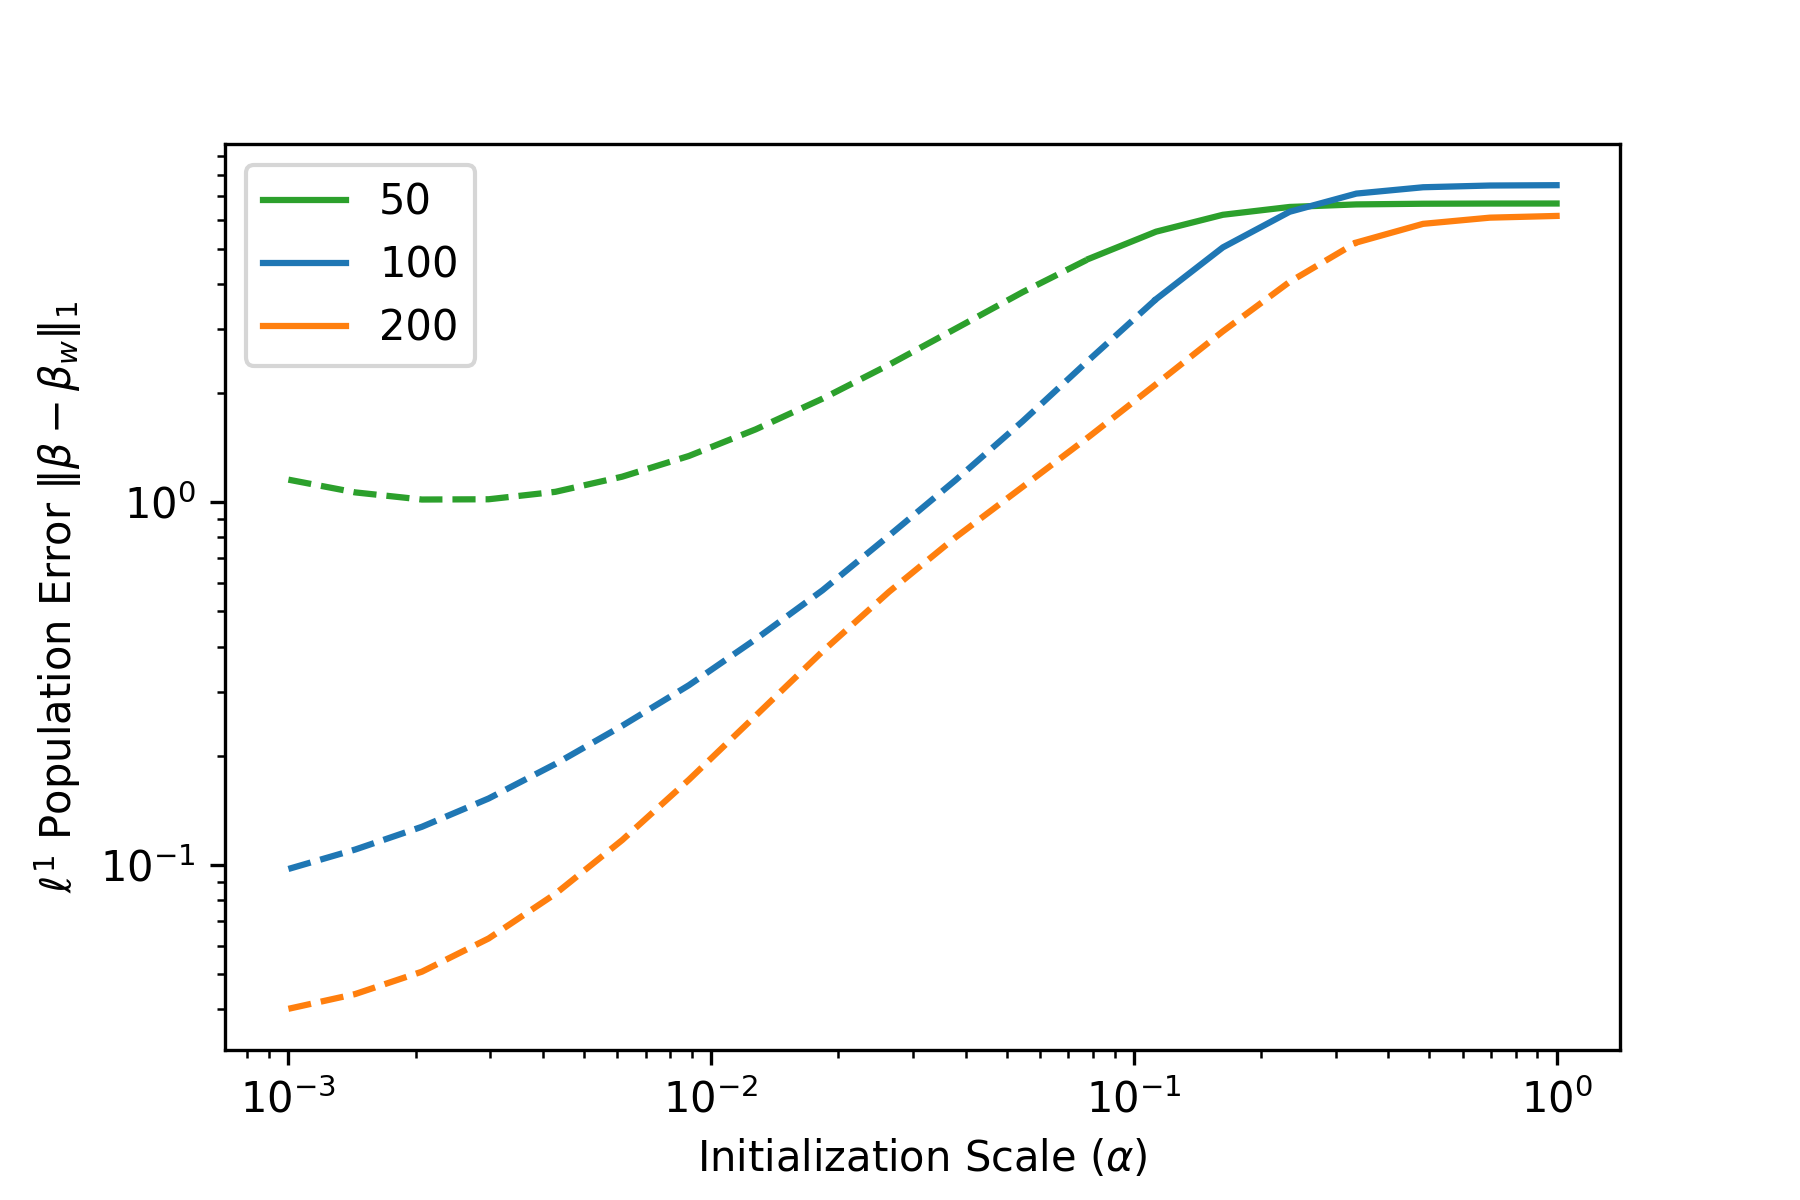
\includegraphics[width=.5\linewidth]{Imgs/Sparse Linear Regression/11_population_error_log_all.png}\label{fig:l1populationerror}}
    \caption{(a) The $\ell^1$ difference between the predictor implemented by gradient descent $\boldsymbol{\beta}_{\boldsymbol{w}_{\alpha}(t_{\text{end}})}$ and the minimum $\ell^1$ solution $\argmin_{\boldsymbol{\beta} \in \mathbb{R}^n} \| \boldsymbol{\beta} \|_1, \ \boldsymbol{X} \boldsymbol{\beta} = \boldsymbol{y}$. (b) The $\ell^1$ difference between the predictor implemented by gradient descent and the ground truth vector $\boldsymbol{\beta}_{\boldsymbol{w}}$ from which the output data is generated. For each of (a) and (b), a dashed line indicates that the gradient descent path did not achieve the specified convergence.}\label{fig:l1error}
\end{figure}

Unlike in our previous experiments, though, we consider the gradient descent path both as a function of the number of training samples, $N$, as well as the initialization scale, $\alpha$. To be more specific, we evaluate the gradient descent path using a training dataset of $N = 50, \ 100,$ and $200$ points $\{ (\boldsymbol{x}_i, y_i) \}_{i=1}^N$. And for each fixed $N$, we choose $20$ logarithmically-spaced values for the initialization scale $\alpha$ on the interval $[10^{-3}, 1]$.

In Figure \ref{fig:excessl1error}, we report the excess $\ell^1$ norm of $\boldsymbol{\beta}_{\boldsymbol{w}_{\alpha}(t_{\text{end}})}$, the predictor implemented at the stopping point of the gradient descent path $(\boldsymbol{w}_{\alpha}(t))_{t \in \mathbb{N}\cup \{0\}}$, $\boldsymbol{w}_{\alpha}(0) = \alpha \mathbbm{1}$. That is, we determine the minimum $\ell^1$ solution to the system $\boldsymbol{X} \boldsymbol{\beta} = \boldsymbol{y}$, denoted $\boldsymbol{\beta}^{\ell^1}$, and then calculate the $\ell^1$ difference between this vector and the predictor implemented by gradient descent $\boldsymbol{\beta}_{\boldsymbol{w}_{\alpha}(t_{\text{end}})}$. From our plot, we see that for each of $N= 100, \ 200$, there is a clear pattern in which the predictor implemented by gradient descent is far from the minimum $\ell^1$ solution for $\alpha =1$ (excess $\ell^1$ norm $\approx5$) but gets significantly closer to this solution as $\alpha$ shrinks towards zero (excess $\ell^1$ norm $\approx 8\times 10^{-1}$ for $\alpha = 10^{-3}$). From our theoretical results regarding the gradient flow solution for the linear regression model in the rich limit $\alpha \rightarrow 0$, this is what we would expect. More explicitly, we know that in the limit $\alpha \rightarrow 0$, the gradient flow solution on the objective $L(h(\boldsymbol{w}))$ with initialization $\boldsymbol{w}_{\alpha}(0) = \alpha \mathbbm{1}$ should correspond exactly to the minimum $\ell^1$ solution of the system $\boldsymbol{X} \boldsymbol{\beta} = \boldsymbol{y}$. On the other hand, since the gradient flow solution in the kernel limit $\alpha \rightarrow \infty$ corresponds to the minimum $\ell^2$ solution, then $\boldsymbol{\beta}_{\boldsymbol{w}_{\alpha}(t_{\text{end}})}$ should not be close to $\boldsymbol{\beta}^{\ell^1}$ for $\alpha$ large.

While the excess $\ell^1$ norm suggests how far the gradient flow solution is from the minimum $\ell^1$ norm solution, we would also like to consider how far it is from the vector $\boldsymbol{\beta}_{\boldsymbol{w}}$ which minimizes the population risk. In Figure \ref{fig:l1populationerror} we present the $\ell^1$ population error, which is measured as the $\ell^1$ distance between $\boldsymbol{\beta}_{\boldsymbol{w}_{\alpha}(t_{\text{end}})}$ and $\boldsymbol{\beta}_{\boldsymbol{w}}$, where $\boldsymbol{\beta}_{\boldsymbol{w}}$ is the vector defined above which determines the distribution of $y_i$. One will notice that unlike $\boldsymbol{\beta}^{\ell^1}$, $\boldsymbol{\beta}_{\boldsymbol{w}}$ is not a solution to the system $\boldsymbol{X} \boldsymbol{\beta} = \boldsymbol{y}$ almost surely. This is a result of the small perturbations made to the output points $y_i$ from their mean $\langle \boldsymbol{\beta}_{\boldsymbol{w}}, \boldsymbol{x}_i \rangle$. Nonetheless, since $\boldsymbol{\beta}_{\boldsymbol{w}}$ is a minimizer of the population risk (\ref{poprisk}), then it is desirable that $\| \boldsymbol{\beta}_{\boldsymbol{w}_{\alpha}(t_{\text{end}})} - \boldsymbol{\beta}_{\boldsymbol{w}} \|_1$ is small. Indeed, we observe that for $N = 100, \ 200$, the $\ell^1$ population error is small for $\alpha$ small: when $\alpha = 10^{-3}$, the $\ell^1$ population error is $\approx 10^{-1}$ with $N=100$ training samples and $\approx 4 \times 10^{-2}$ with $N=200$ training samples. Intuitively, we would suspect that $\boldsymbol{\beta}_{\boldsymbol{w}_{\alpha}(t_{\text{end}})}$ should be close to $\boldsymbol{\beta}_{\boldsymbol{w}}$ for $\alpha$ small since $\boldsymbol{\beta}_{\boldsymbol{w}}$ itself is sparse. This informs how one should choose their initialization scale to minimize the population risk when they believe that the underlying data distribution is sparse.

\begin{figure}[H]
    \centering
    \subfloat[$\alpha = 10^{-3}$]{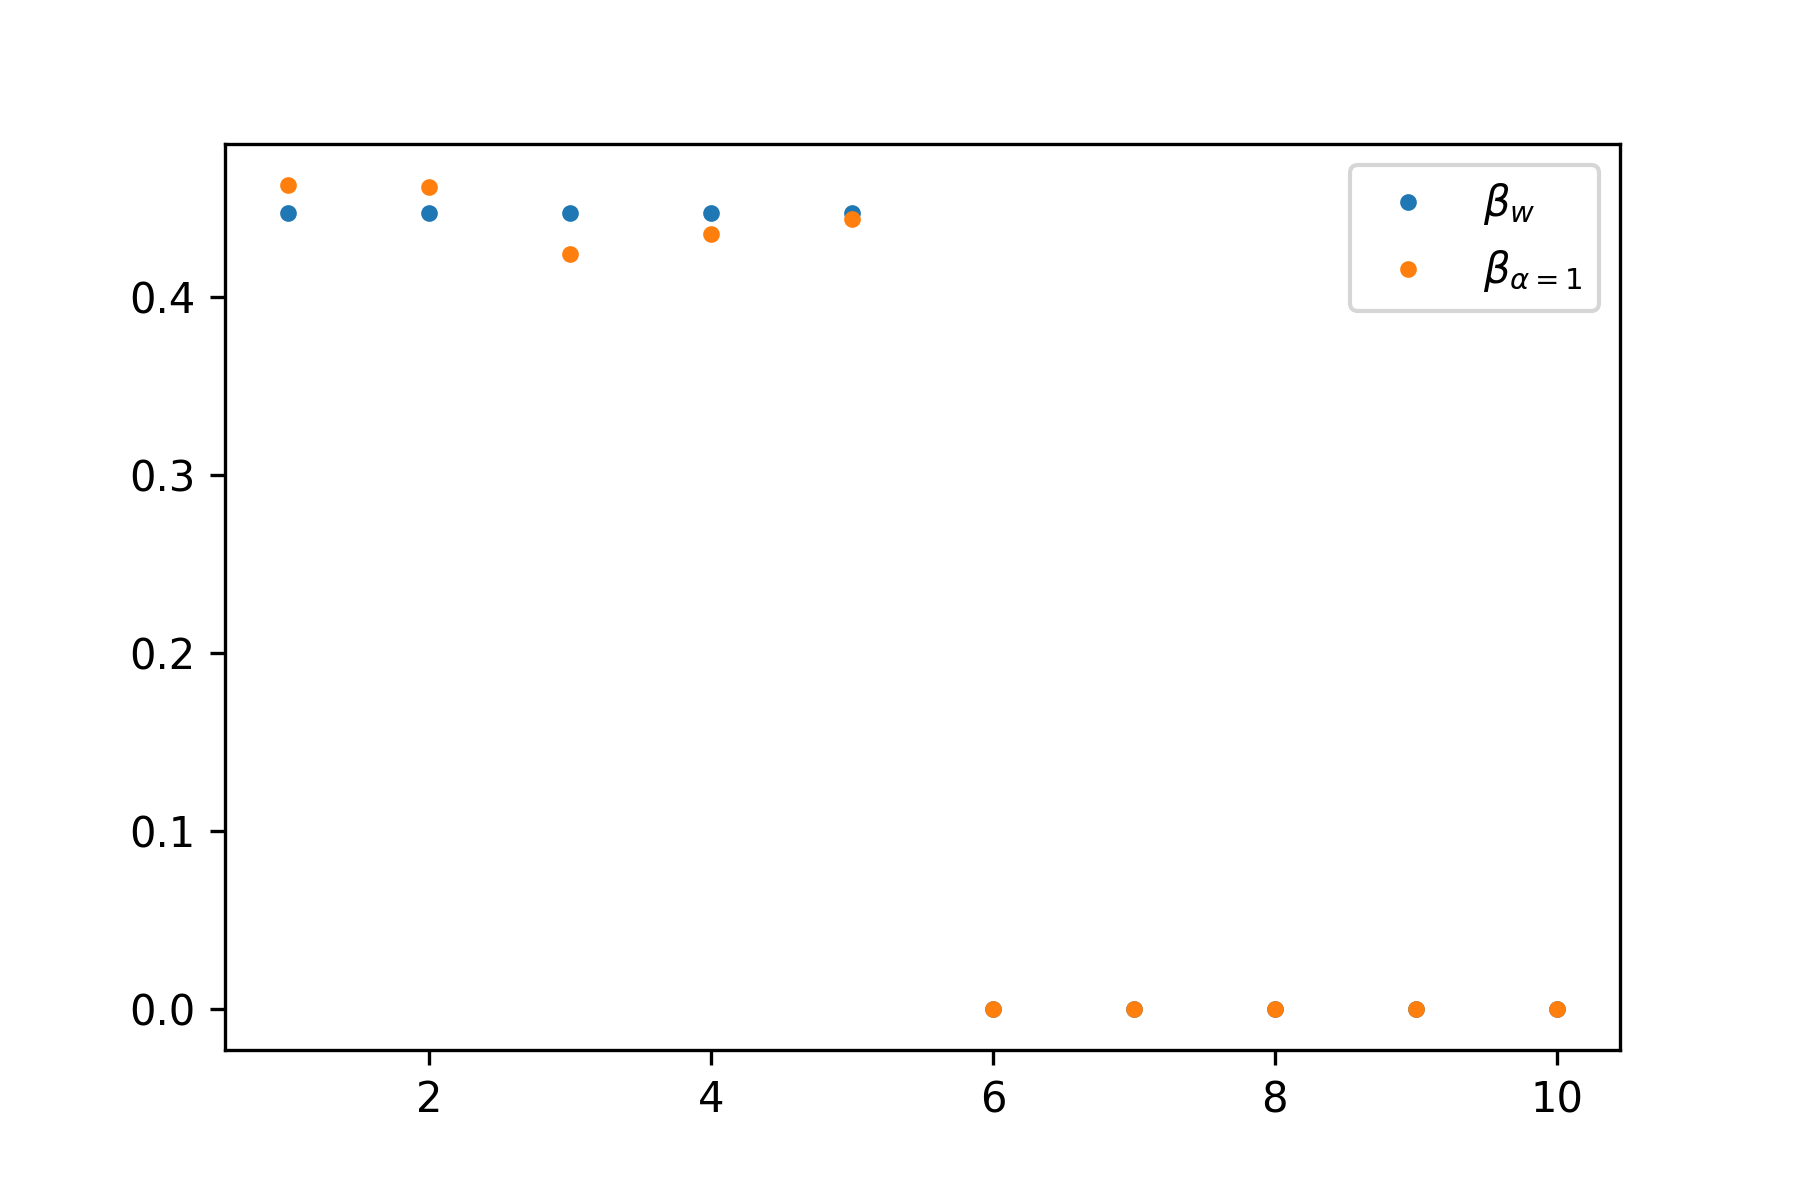
\includegraphics[width=.5\linewidth]{Imgs/Sparse Linear Regression/visualize_solution_vec_0.001.png}\label{}}\hfill
    \subfloat[$\alpha =1$]{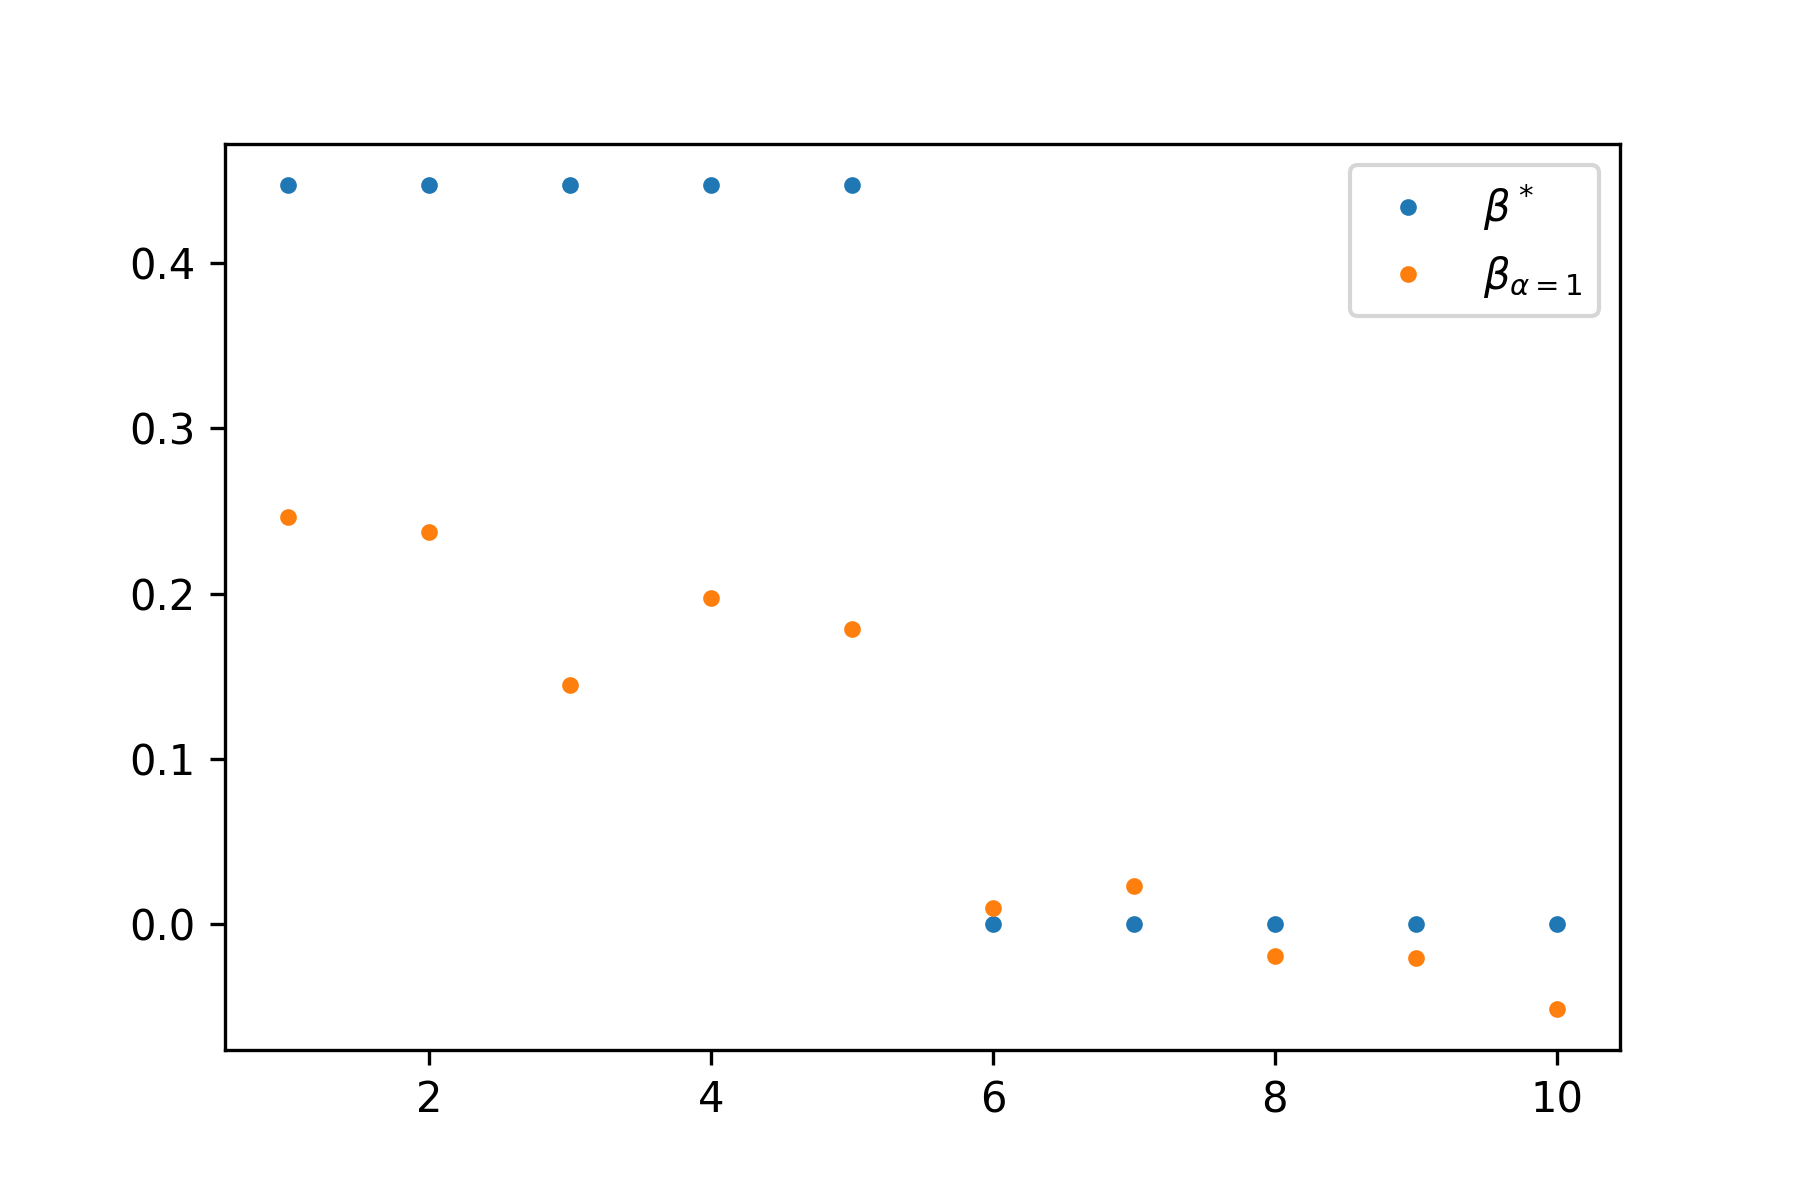
\includegraphics[width=.5\linewidth]{Imgs/Sparse Linear Regression/visualize_solution_vec_1.png}\label{}}
    \caption{The first 10 coordinates of the gradient descent solution vector $\boldsymbol{\beta}_{\boldsymbol{w}_{\alpha}(t_{\text{end}})}$ (orange) and those of the ground truth vector $\boldsymbol{\beta}_{\boldsymbol{w}}$ (blue). Gradient descent is performed using $N=100$ training points.}\label{fig:solutionpts}
\end{figure}

To better visualize how the gradient flow solution changes as a function of the initialization scale, we plot the first 10 coordinates of $\boldsymbol{\beta}_{\boldsymbol{w}_{\alpha}(t_{\text{end}})}$ against those of $\boldsymbol{\beta}_{\boldsymbol{w}}$ for each of $\alpha = 10^{-3}$ and $\alpha = 1$. What first sticks out to us is that the gradient descent solution corresponding to $\alpha = 1$ is not sparse. Although the solution vector certainly exhibits shrinkage of the second five coordinates, they are not close to zero as they are in $\boldsymbol{\beta}_{\boldsymbol{w}}$. For the $\alpha = 10^{-3}$ solution vector, on the other hand, we do observe that the second five coordinates are all nearly zero. Also, the gradient descent solution picks out the first five coordinates as those which are most important for predicting $y_i$, as is the case in the ground truth vector $\boldsymbol{\beta}_{\boldsymbol{w}}$. Not only does it identify these coordinates, but $(\boldsymbol{\beta}_{\boldsymbol{w}_{\alpha}(t_{\text{end}})})_i$ is very close to the $(\boldsymbol{\beta}_{\boldsymbol{w}})_i = 1/\sqrt{5}$ for $1 \leq i \leq 5$. 

It is also worth mentioning that these experimental results agree with those originally reported by Woodworth and colleagues in \cite{woodworth2020kernel}. We carefully chose our input dimension $n$, data distribution $\rho$, and learning rate $\eta$ to match with those used by the authors in Figures 1(c) and 3(c). The problem considered in Figures 1(a) and 1(b) uses $N=100$ training samples, just as we did, but has higher input dimension, $d=10^3$, than that which we considered. Irrespective of this difference in dimension, we observe the same relationship between the initialization scale $\alpha \in \mathbb{R}_{++}$ of the gradient descent path $(\boldsymbol{w}_{\alpha}(t))_{t \geq 0}$ and the population error. Expressly, the authors illustrate that beginning at $\alpha \approx 10^{-1}$ there is a sharp decrease in the population error $\| \boldsymbol{\beta}_{\boldsymbol{w}_{\alpha}(t_{\text{end}})} - \boldsymbol{\beta}_{\boldsymbol{w}} \|_2^2$. And as the initialization scale $\alpha \rightarrow 0$, the population error appears to decrease monotonically towards $0$, albeit at a slower rate. One will notice that the definition of \enquote{population error} adopted by Woodworth and colleagues, the $\ell^2$ distance between $\boldsymbol{\beta}_{\boldsymbol{w}_{\alpha}(t_{\text{end}})}$ and $\boldsymbol{\beta}_{\boldsymbol{w}}$, differs from that we report in Figure \ref{fig:l1populationerror}. 

Similarly, in Figure 1(b) of \cite{woodworth2020kernel}, the authors plot the excess $\ell^1$ norm of the predictor implemented by gradient descent $\boldsymbol{\beta}_{\boldsymbol{w}_{\alpha}(t_{\text{end}})}$. Just as we see from our own experiments in Figure \ref{fig:excessl1error}, starting once again at around $\alpha \approx 10^{-1}$, there is a sharp decrease in the excess $\ell^1$ norm. It then appears to continue decreasing monotonically as $\alpha \rightarrow 0$. As we have mentioned before, because we know that $\boldsymbol{\beta}_{\alpha}^{\star} \rightarrow \boldsymbol{\beta}^{\ell^1}$ as $\alpha \rightarrow \infty$, where $\boldsymbol{\beta}_{\alpha}^{\star} = \lim_{t \to \infty} \boldsymbol{\beta}_{\boldsymbol{w}_{\alpha}(t)}$, then we would expect the excess $\ell^1$ norm of the gradient descent solution to approach $0$ as $\alpha \rightarrow 0$.

In summary, reproducing the work of Woodworth and colleagues, we have suggested a problem in which training near the rich limit is preferable to training near the kernel limit. In particular, we have shown that for the linear regression problem (\ref{linreg}), the rich limit corresponds to the minimum $\ell^1$ solution to the system $\boldsymbol{X}\boldsymbol{\beta} = \boldsymbol{y}$, whereas the kernel limit corresponds to the minimum $\ell^2$ solution. Accordingly, we would expect that for problems in which the underlying data distribution $\rho$ is sparse, training our network $f(\boldsymbol{w}, \boldsymbol{x})$ near the rich limit would achieve smaller population risk than had the model been trained near the rich limit.

\subsubsection{Computational Limitations of Rich Training}
So far in the discussion of our results we have ignored an obvious deficiency in rich training. Patently, in Figure \ref{fig:l1error} we observe that for $\alpha$ small, the loss of the gradient flow descent path $L(h(\boldsymbol{w}_{\alpha}(t)))$ does not converge within $10^{-4}$ of the global minimum loss value, $0$. In fact, we only see this convergence for $\alpha \approx 1$, which is quite a large initialization scale (i.e.~is closer to the kernel limit). Also, we observe that for the gradient descent path with $N=50$ training samples, the excess $\ell^1$ norm and $\ell^1$ population error begin to increase for sufficiently small $\alpha$. This belies our previous assertion that both the excess $\ell^1$ norm and $\ell^1$ population error monotonically decrease as $\alpha \rightarrow 0$.

These seemingly anomalous results can be attributed to two facts about the problem. First, as we have previously pointed out, gradient descent is a discretization of the gradient flow dynamics, and so we would expect the gradient descent path to differ from the corresponding gradient flow. This is why I suspect the excess $\ell^1$ norm and $\ell^1$ population error begin to increase for the gradient descent path with $N=50$: when the initialization scale is very small, and so the gradient descent is initialized with $\boldsymbol{w}_{\alpha}(0) \approx \boldsymbol{0}$, a very small stepsize is necessary to attain convergence. 

Beyond just the coarseness of the stepsize, though, there is another aspect of the optimization problem that makes training close to the rich limit intractable. Namely, as one may have guessed from Figure \ref{linearizedmodel}, the objective $L(h(\boldsymbol{w}))$ often has a saddle point at $\boldsymbol{w} = \boldsymbol{0}$ \cite{woodworth2020kernel}. Therefore by taking $\alpha \rightarrow 0$ in the rich limit, we are initializing the weight vector closer and closer to a saddle point of $L(h(\boldsymbol{w}))$. Undoubtedly, this small initialization complicates the optimization problem since it takes longer and longer for the gradient flow path to escape the vicinity of the saddle point. We conjecture that this is exactly the problem we are facing in our simulation: for $\alpha$ small, we are not able to escape the saddle point within the specified $10^4$ epochs. In fact, for $\alpha$ sufficiently small, we would not expect the gradient flow path to ever depart from $\boldsymbol{0}$ within any reasonable amount of time. 

This reality of training in the rich regime gives rise to a tradeoff between optimization and generalization as characterized by Woodworth and colleagues \cite{woodworth2020kernel}. That is, in practice, one must choose $\alpha$ sufficiently small to train near the rich limit and achieve the corresponding $\ell^1$ implicit regularization in the network weights. Yet, one must avoid training with $\alpha$ too small or else the gradient descent path will never escape the saddle point $\boldsymbol{0}$ and attain the desired convergence.

\subsection{A New Problem: Sparse Binary Classification}\label{sparselogistic}
In Sections \ref{richkerneltheory} and \ref{sparselinear}, we illustrated both theoretically and experimentally that for the linear regression problem (\ref{linreg}), the kernel limit $\lim_{\alpha \to \infty}\boldsymbol{\beta}_{\alpha}^{\star}$ corresponds to the minimum $\ell^2$ solution of the linear system $\boldsymbol{X} \boldsymbol{\beta} = \boldsymbol{y}$, whereas the rich limit $\lim_{\alpha \to 0}\boldsymbol{\beta}_{\alpha}^{\star}$ corresponds to the minimum $\ell^1$ solution \cite{woodworth2020kernel}. Consequently, for problems in which the population risk (\ref{poprisk}) can be minimized by a sparse weight vector, we would prefer training near the rich limit to training near its kernel counterpart. 

Although this result is of significant merit, contemporary network architectures are substantially more complicated than the single-layer network we considered. Almost all practical networks are not differentiable in their weights $\boldsymbol{w} \in \mathbb{R}^p$. Consider, for example, the ReLU nonlinearity $\max\{0, x \}$ applied element-wise to the output of the hidden layers of our network $f$. Also, neural networks are often initialized with random weights, and so they do not vanish at their initialization. Hence, the results we stated from Chizat and colleagues cannot be applied to most interesting deep learning problems \cite{chizat2019lazy}. 

Still, as articulated by Woodworth and colleagues, we suspect that some of the behaviors we observe in the kernel and rich regimes do exist for these nondifferentiable problems. To be explicit, we conjecture that there exists a rich limit which corresponds to some form of implicit $\ell^1$ regularization, as it did for the linear regression problem. In the next section, we will discuss the presence of \enquote{rich} training in the binary classification problem posed by Wei and colleagues \cite{wei2019regularization}. Moreover, we will address the question of whether rich training in the binary classification problem results in desirable generalization when the data is sparse, as was the case for the linear regression problem (\ref{linreg}). 

We will no longer maintain the assumption stated in Section \ref{preliminaries} that the model $h: \boldsymbol{w} \mapsto f(\boldsymbol{w}, \boldsymbol{x})$ is differentiable, nor the assumption that the model is identically zero its initialization. This means that the gradient flow paths of $L(h(\boldsymbol{w}))$ and $L(\bar{h}(\boldsymbol{w}))$ with $\boldsymbol{w}_{\alpha}(0) = \boldsymbol{\bar{w}}_{\alpha}(0) = \alpha \boldsymbol{w}_0$ do not necessarily exist. If $L(h(\boldsymbol{w}))$ is subdifferentiable, we could employ a subgradient method instead.

\subsubsection{Binary Classification Problem}

The model we describe was originally proposed by Wei and colleagues in \cite{wei2019regularization}. Consider data $(\boldsymbol{x}, y) \sim \rho$ for $\boldsymbol{x} \in \mathcal{X} = \{ +1, 0, -1 \}^n$, $y \in \{+1, -1\}$. The distribution $\rho$ is defined such that 
\begin{align*}
    &y = +1, \quad \boldsymbol{x}^Te_1 = +1, \quad \boldsymbol{x}^Te_2 = 0 \quad \text{w/ prob. 1/4}\\
    &y = +1, \quad \boldsymbol{x}^Te_1 = -1, \quad \boldsymbol{x}^Te_2 = 0 \quad \text{w/ prob. 1/4}\\
    &y = -1, \quad \boldsymbol{x}^Te_1 = 0, \quad \boldsymbol{x}^Te_2 = +1 \quad \text{w/ prob. 1/4}\\
    &y = -1, \quad \boldsymbol{x}^Te_1 = 0, \quad \boldsymbol{x}^Te_2 = -1 \quad \text{w/ prob. 1/4}
\end{align*}
and $\boldsymbol{x}^Te_i \sim \{+1, -1 \}$ is drawn uniformly at random for $3 \leq i \leq n$. From this definition of $\rho$, it should be clear that the output $y$ is entirely determined by the first two coordinates of the input vector $\boldsymbol{x}$.

To associate a model with this data distribution $\rho$, the authors investigate the case of $h(\boldsymbol{w}) = f(\boldsymbol{w}, \boldsymbol{x})$ a single-hidden-layer ReLU neural network with $m$ neurons:
\begin{align}\label{relunn}
    f(\boldsymbol{w}, \boldsymbol{x}) = \sum_{i=1}^m v_j[\boldsymbol{u}_j^T\boldsymbol{x}]_+.
\end{align}
Here, $[\cdot]_+$ denotes the ReLU activation $\max\{0, x \}$ and $\boldsymbol{w}$ is the collection of all $m \times (n+1)$ parameters $\{ (v_j, \boldsymbol{u}_j) \}_{i=1}^m$. Unlike the weights of the linear regression model, which are initialized deterministically, the weights of the ReLU neural network (\ref{relunn}) are initialized randomly: $v \sim \mathcal{N}(0, r_v^2)$ and $\boldsymbol{u} \sim \mathcal{N}(\boldsymbol{0}, r_{\boldsymbol{u}}^2\mathbbm{I}_{n \times n})$ \cite{wei2019regularization}. Also, we point out that the ReLU neural network is 2-positive homogeneous in its weights $\boldsymbol{w}$. 

Since our outputs are binary labels, we take $L$ to be the empirical risk corresponding to the logistic loss 
\begin{align}\label{logloss}
    L(f(\boldsymbol{w}, \boldsymbol{x})) = \mathbb{E}_{(\boldsymbol{x}, y) \sim \mathcal{D}} \left[\log \left( 1 + \exp(-y f(\boldsymbol{w}, \boldsymbol{x})) \right) \right] = \frac{1}{N} \sum_{i=1}^N \log \left( 1 + \exp(-y_i f(\boldsymbol{w}, \boldsymbol{x}_i)) \right),
\end{align}
where $\mathcal{D}$ is the empirical distribution determined by the training data $\{ (\boldsymbol{x}_i, y_i) \}_{i=1}^N$ \cite{wei2019regularization}. We let $(\boldsymbol{w}_{r_v, r_{\boldsymbol{u}}}(t))_{t \geq 0}$ denote the gradient flow path on the objective function $L(h(\boldsymbol{w}))$ with $v_j(0) \sim \mathcal{N}(0, r_v^2)$, $\boldsymbol{u}_j(0) \sim \mathcal{N}(0, r_{\boldsymbol{u}}^2)$.

Under our assumption that $\lim_{t \to \infty} L(h(\boldsymbol{w}_{r_v, r_{\boldsymbol{u}}}(t))) = 0$, then it must be the case that $y_i f(\boldsymbol{w}_{r_v, r_{\boldsymbol{u}}}(t'), \boldsymbol{x}_i) > 0$ for all $i=1,\ldots, N$ at some time $t' \in \mathbb{R}_+$. In other words, our neural network must classify all training points correctly at some time in the gradient flow trajectory. Also, we know that $\lim_{t \to \infty} \Vert \boldsymbol{w}_{r_v, r_{\boldsymbol{u}}}(t) \Vert_2\\ = +\infty$. This means that the loss of the model implemented by our gradient flow path tends to zero while the individual weights of the model diverge in the $\ell^2$ sense.

And so since the limit of the gradient flow does not exist, we instead consider the \textit{direction} of the gradient flow, $\boldsymbol{w}_{r_v, r_{\boldsymbol{u}}}(t)/\Vert \boldsymbol{w}_{r_v, r_{\boldsymbol{u}}}(t) \Vert_2$, in the limit as $t \rightarrow \infty$. Ji and Telgarsky proved that for neural networks with an arbitrary number of linear, ReLU, max-pooling, and convolutional hidden layers, the direction of the gradient flow path converges, provided the network classifies all training points correctly at some time in its gradient flow trajectory (see Theorem 3.1 in \cite{ji2020directional}). We know that for our problem setup and assumptions, $\boldsymbol{w}_{r_v, r_{\boldsymbol{u}}}^{\star} = \lim_{t \to \infty} \frac{\boldsymbol{w}_{r_v, r_{\boldsymbol{u}}}(t)}{\Vert \boldsymbol{w}_{r_v, r_{\boldsymbol{u}}}(t) \Vert_2}$ exists.\footnote{At the time of writing my thesis, I was not knowledgeable about the theory surrounding rich training for binary classification problems, and so my work is lacking in this regard. I point readers in the direction of a few influential papers on this topic: \enquote{Gradient Descent Maximizes the Margin of Homogeneous Neural Networks} by Lyu and Li \cite{lyu2019gradient}, \enquote{Directional Convergence and Alignment in Deep Learning} by Ji and Telgarsky \cite{ji2020directional}, \enquote{The Implicit Bias of Gradient Descent on Separable Data} by Soudry and colleagues \cite{soudry2018implicit}, and \enquote{Implicit Bias of Gradient Descent on Linear Convolutional Networks} by Gunasekar and colleagues \cite{gunasekar2018implicitconv}. Still, my research is novel insofar as it considers the implicit bias resulting from rich training for finite-width ReLU neural networks. Chizat and Bach studied the implicit bias for ReLU neural networks in the infinite width case and showed that in the rich regime, the predictor implemented by gradient flow is a max-margin variational norm solution \cite{chizat2020implicit}.}

Having given both the data distribution $\rho$ and the model $h: \boldsymbol{w} \mapsto f(\boldsymbol{w}, \boldsymbol{x})$, we now justify that the problem we have defined is indeed sparse. In the case of the linear regression problem (\ref{linreg}), we discussed sparsity in the space of predictors $\mathcal{F} = (\mathbb{R}^n)^*$. However, for the binary classification problem, our Hilbert space $\mathcal{F}$ is a much more complex function class; in particular, it contains functions that are nonlinear in the input. For this reason, we discuss sparsity in the parameter space $\mathbb{R}^{m\times(n+1)}$ rather than the predictor space.

If we choose $\boldsymbol{w}$ such that $\boldsymbol{u}_1 = e_1$, $\boldsymbol{u}_2 = -e_1$, $\boldsymbol{u}_3 = e_2$, $\boldsymbol{u}_4 = -e_2$, and $v_1 = v_2 = +1$, $v_3 = v_4 = -1$ then $\boldsymbol{w}$ minimizes $\boldsymbol{w} \mapsto \mathbb{E}_{(\boldsymbol{x}, y) \sim \rho} [\mathbbm{1}_{f(\boldsymbol{w}, \boldsymbol{x})y \leq 0}] = \mathbb{P}(f(\boldsymbol{w}, \boldsymbol{x})y \leq 0)$ \cite{wei2019regularization}. This specific weight vector $\boldsymbol{w}$ that minimizes the population risk contains only eight nonzero weights, meaning that our problem is indeed sparse according to our previous definition. Here, we are considering the population risk corresponding to the binary $\{0, +1\}$ loss $\ell(y, y') = \mathbbm{1}_{y \cdot y' \leq 0}$, rather than the logistic loss defined above. This is because, as we mentioned above, the empirical risk corresponding the logistic loss is minimized at no finite-norm weight vector $\boldsymbol{w}$. In particular, for any $\boldsymbol{\tilde{w}} \in \mathbb{R}^{m \times (n+1)}$ satisfying $y_i f(\boldsymbol{\tilde{w}}, \boldsymbol{x}_i) > 0$ for all $i = 1, \ldots, N$, then $L(f(\alpha \boldsymbol{\tilde{w}}, \boldsymbol{x})) < L(f(\boldsymbol{\tilde{w}}, \boldsymbol{x}))$ whenever $\alpha > 1$. This implies that we can minimize the loss by scaling this weight vector $\boldsymbol{\tilde{w}}$ to have arbitrarily large norm: $\lim_{\alpha \to \infty} L(f(\alpha \boldsymbol{\tilde{w}}, \boldsymbol{x})) = 0$.

Prior to experimenting with the binary classification problem from \cite{wei2019regularization}, we provide more context for the authors' work and comment on how it relates to our research. First, Wei and colleagues provide an explicit characterization of the neural tangent kernel at the network's initialization:
\begin{align*}
    K_{\boldsymbol{w}_{r_v, r_{\boldsymbol{u}}}(0)}(\boldsymbol{x}, \boldsymbol{x}') = \mathbb{E}_{v \sim \mathcal{N}(0, r_v), \ \boldsymbol{u} \sim \mathcal{N}(0, r_{\boldsymbol{u}}^2)}[ \left\langle \nabla_{(v, \boldsymbol{u})}f(\boldsymbol{w}, \boldsymbol{x}), \nabla_{(v, \boldsymbol{u})}f(\boldsymbol{w}, \boldsymbol{x}') \right\rangle]
\end{align*}
where $\nabla_{(v, \boldsymbol{u})}f(\boldsymbol{w}, \boldsymbol{x}) = ([\boldsymbol{u}^T\boldsymbol{x}]_+, v\mathbbm{1}_{\boldsymbol{u}^T\boldsymbol{x} \geq 0}\boldsymbol{x}) \in \mathbb{R}^{n + 1}$ is the gradient of $f$ with respect to an arbitrary pair of weights $(v, \boldsymbol{u})$ (since they are initialized \textit{i.i.d.}). We point out that for $\boldsymbol{u}^T\boldsymbol{x}=0$, $\nabla_{(v, \boldsymbol{u})}f(\boldsymbol{w}, \boldsymbol{x})$ does not exist, although $([\boldsymbol{u}^T\boldsymbol{x}]_+, v\boldsymbol{x})$ is contained in the subdifferential of $f$ at $(v, \boldsymbol{u})$. Although the neural tangent kernels corresponding to the linear regression model (\ref{linreg}) and ReLU neural network (\ref{relunn}) are both deterministic at their initializations, the latter involves evaluating an expectation over the distribution of weight initializations $(v, \boldsymbol{u})$.

Wei and colleagues are interested in the neural tangent kernel $K_{\boldsymbol{w}_{r_v, r_{\boldsymbol{u}}}(0)}$ at the network's initialization because they study the predictor functions $f^{\text{kernel}}$ in the corresponding RKHS $H_{\varphi_{\boldsymbol{w}_{r_v, r_{\boldsymbol{u}}}(0)}}$: 
\begin{align*}
f^{\text{kernel}}(\boldsymbol{x}, \boldsymbol{\gamma}) = \sum_{i=1}^N \boldsymbol{\gamma}_i K_{\boldsymbol{w}_{r_v, r_{\boldsymbol{u}}}(0)}(\boldsymbol{x}_i, \boldsymbol{x}).
\end{align*}
From the theory of Jacot and colleagues \cite{jacot2018neural}, we know that by performing gradient descent in the infinite-width limit $m \rightarrow \infty$, one would obtain such a predictor $f^{\text{kernel}}$.

Now that we have introduced $f^{\text{kernel}}$, we state the main result formulated and proven and proven by Wei and colleagues: 
\begin{manualtheorem}{2.1}[from \cite{wei2019regularization}]\label{weithm2.1}
Let $\rho$ be the distribution defined previously. With probability $1 - n^{-5}$ over the random draw of $N \lesssim n^2$ samples $(x_1, y_1), \ldots, (x_N, y_N)$ from $\rho$, for all choices of $\boldsymbol{\gamma}$, the kernel prediction function $f^{\text{kernel}}(\cdot, \boldsymbol{\gamma})$ will have at least $\Omega(1)$ error
\begin{align*}
    \mathbb{P}_{(\boldsymbol{x}, y) \sim \rho}[f^{\text{kernel}}(\boldsymbol{x}; \boldsymbol{\gamma})y \leq 0] = \Omega(1).
\end{align*}
Moreover, let us define the $\ell^2$ regularized logistic loss $L_{\lambda}$
\begin{align*}
    L_{\lambda}(f(\boldsymbol{w}, \boldsymbol{x})) = \mathbb{E}_{(\boldsymbol{x}, y) \sim \mathcal{D}} \left[\log \left( 1 + \exp(-y f(\boldsymbol{w}, \boldsymbol{x})) \right) \right] + \lambda \|\boldsymbol{w} \|_F^2,
\end{align*}
where $\boldsymbol{w} \in \mathbb{R}^{m \times (n+1)}$, $\boldsymbol{w}_{i,:} = (v_i, \boldsymbol{u}_i)$ is the matrix containing the network parameters. Then for $\lambda \leq \text{poly}(N)^{-1}$, the regularized neural net solution $f(\boldsymbol{w}_{\lambda}, \boldsymbol{x})$ trained with at least four hidden units can have good approximation with $\mathcal{O}(n^2)$ samples because we have the following generalization error bound:
\begin{align*}
   \mathbb{P}_{(x,y) \sim \rho}[f(\boldsymbol{w}_{\lambda}, \boldsymbol{x})y \leq 0] \lesssim \sqrt{\frac{n}{N}}.
\end{align*}
This implies a $\Omega(n)$ sample-complexity gap between the regularized neural net and kernel prediction function.
\end{manualtheorem}
Plainly, Theorem \ref{weithm2.1} states that the gradient descent on the $\ell^2$ regularized objective $L_{\lambda}(f(\boldsymbol{w}, \boldsymbol{x}))$ achieves a model which generalizes well over the population distribution of data $\rho$ with only $n^2$ samples, whereas any estimator contained in $H_{\varphi_{\boldsymbol{w}_{r_v, r_{\boldsymbol{u}}}(0)}}$ does not.

As we have previously discussed, we know that there exists implicit $\ell^0$ sparsity in the binary classification problem we have posed: using only eight nonzero weights, one can minimize the population risk $\mathbb{P}_{(\boldsymbol{x}, y) \sim \rho} \left[ y f(\boldsymbol{w}, \boldsymbol{x}) \leq 0 \right]$. To impose this sparsity in their gradient flow solution, Wei and colleagues utilize an explicit $\ell^2$ regularizer in their loss function $L_{\lambda}$. However, considering the analogy of regularized least-squares problems, we know that $\ell^1$ regularization serves as a much better proxy for $\ell^0$ sparsity than its $\ell^2$ counterpart.

Therefore, we would expect that under the aforementioned data distribution $\rho$, Wei and colleagues could have attained a better generalization error bound on $f(\boldsymbol{w}_{\lambda}, \boldsymbol{x})$ had they included an $\ell^1$, as opposed to $\ell^2$, regularizer in the loss. However, this also raises the question of whether, similar to the linear regression model (\ref{linreg}), there exists a \enquote{rich} training regime in which the weights of the network are subjected to some form of implicit $\ell^1$ regularization. If so, we would expect the model trained in this rich setting to have generalization properties that are comparable to, or even better than, those in Theorem \ref{weithm2.1}. In Section \ref{richbinary}, we discuss what this rich regime may look like, and we then perform computational experiments to demonstrate how it manifests in training.

\subsubsection{The Rich Limit for Binary Classification}\label{richbinary}

The rich limit in the binary classification problem we have posed is much different from that corresponding to the linear regression problem discussed in Section \ref{linregmodel}. In particular, Lyu and Li proved that for our binary classification problem, rich training occurs at \textit{all finite initialization scales} \cite{lyu2019gradient}. That is, the implicit biases to which the gradient flow path $(\boldsymbol{w}_{r_v, r_{\boldsymbol{u}}}(t))_{t \geq 0}$ is subjected does not depend on $r_v, r_{\boldsymbol{u}} \in \mathbb{R}_{+}$. The reader will recall that this is very different from linear regression, wherein we interpolate between the rich and kernel limits depending on the initialization scale $\alpha \in \mathbb{R}_{++}$ (see Theorem 1 in \cite{woodworth2020kernel}). 

However, what the result by Lyu and Li does not tell us is the rate at which the gradient flow direction $\frac{\boldsymbol{w}_{r_v, r_{\boldsymbol{u}}}(t)}{\Vert \boldsymbol{w}_{r_v, r_{\boldsymbol{u}}}(t) \Vert_2}$ converges. We hypothesize that for large initialization scale $r_v, r_{\boldsymbol{u}}$, gradient flow on $L(h(\boldsymbol{w}))$ behaves similar to a kernel method early-on during training before eventually converging to its rich limit. For this reason, we will refer to the \enquote{rich limit} as $\lim_{t \to \infty} \lim_{r_v, r_{\boldsymbol{u}} \to 0} \frac{\boldsymbol{w}_{r_v, r_{\boldsymbol{u}}}(t)}{\Vert \boldsymbol{w}_{r_v, r_{\boldsymbol{u}}}(t) \Vert_2}$. We believe that in this limit, gradient flow behaves very differently from a kernel method throughout the entirety of training, not just in its limit. As we will see in Section \ref{logregcomputation}, it does appear that when stopping gradient flow at a finite time $t_{\text{end}} \in \mathbb{R}_+$, small initialization scales $r_v, r_{\boldsymbol{u}}$ demonstrate, in some sense, richer behaviors.

Moreover, as we suggested in the previous section, we might expect that rich training for the binary classification problem corresponds to some implicit $\ell^1$ regularization in the weight vector $\boldsymbol{w} \in \mathbb{R}^{m \times (n+1)}$. This is different from our discussion of implicit regularization for the linear regression problem, wherein the linear predictor itself, rather than the network weights, are subject to regularization. In other words, we will be discussing regularization in the parameter space rather than the predictor space.

To conclude our discussion of the rich regime for binary classification, we point out that it is not necessarily true that gradient flow is equivalent to a kernel method in the limit $r_v, r_{\boldsymbol{u}} \rightarrow \infty$. This is because by initializing our weights randomly, our model $f(\boldsymbol{w}, \boldsymbol{x})$ will not be identically zero at its initialization. Therefore, the results proven by Chizat and colleagues, Theorems \ref{Chizatthm2.2} and \ref{Chizatthm2.4}, do not hold. For this reason, we will only discuss the \enquote{rich regime} and \enquote{rich limit,} not the \enquote{kernel regime} and \enquote{kernel limit.}


\subsubsection{Computational Experiments Near the Rich Limit}\label{logregcomputation}

From the previous section, we know that rich training for the binary classification problem occurs at all finite initialization scales $r_v, r_{\boldsymbol{u}}$. Still, because we cannot run gradient flow for arbitrarily long, we are interested in values of $r_v, r_{\boldsymbol{u}}$ for which $\frac{\boldsymbol{w}_{r_v, r_{\boldsymbol{u}}}(t)}{\Vert \boldsymbol{w}_{r_v, r_{\boldsymbol{u}}}(t) \Vert_2}$ converges faster to its limit. Next, we explore the possibility that training the ReLU neural network (\ref{relunn}) near the rich limit for the sparse binary classification problem corresponds to implicit $\ell^1$ regularization in the parameter space. We do so by conducting a couple of experiments.

Explicitly, we will consider the gradient descent path $(\boldsymbol{w}_{r_v, r_{\boldsymbol{u}}}(t))_{t \in \mathbb{N} \cup \{0\}}$ with $\boldsymbol{w}_{r_v, r_{\boldsymbol{u}}}(0)$ initialized according to $v_i \sim \mathcal{N}(0, r_v^2)$, $\boldsymbol{u}_i \sim \mathcal{N}(\boldsymbol{0}, r_{\boldsymbol{u}}^2 \mathbbm{I}_{n \times n})$ for each hidden unit $1 \leq i \leq m$. Differing from our experiments in Section \ref{sparselinear}, the starting point of the gradient descent path is random. Accordingly, rather than simulating gradient descent once for each $r_v, r_{\boldsymbol{u}}$, we consider $K$ gradient descent paths, each of which is initialized with a random starting point $\boldsymbol{w}_{r_v, r_{\boldsymbol{u}}}(0)$. This implies that the limiting gradient flow direction itself, $\boldsymbol{w}_{r_v, r_{\boldsymbol{u}}}^{\star} = \lim_{t \to \infty} \frac{\boldsymbol{w}_{r_v, r_{\boldsymbol{u}}}(t)}{\Vert \boldsymbol{w}_{r_v, r_{\boldsymbol{u}}}(t) \Vert_2}$, is random. 

Therefore, the population risk is $\mathbb{P}_{(x,y) \sim \rho, v_i, \boldsymbol{u}_i}[f(\boldsymbol{w}_{r_v, r_{\boldsymbol{u}}}^{\star}, \boldsymbol{x})y \leq 0]$. For each $r_v, r_{\boldsymbol{u}}$, we estimate the risk by averaging over the test error for each of $K$ gradient descent paths. That is, the estimated population risk is
\begin{align*}
    \frac{1}{KN_{\text{test}}}\sum_{k=1}^K \sum_{i=1}^{N_{\text{test}}} \mathbbm{1}_{y_i f\left(\boldsymbol{w}_{r_v, r_{\boldsymbol{u}}}^{(k)}(t_{\text{end}}), \boldsymbol{x}_i\right) \leq 0}
\end{align*}
where $\left(\boldsymbol{w}_{r_v, r_{\boldsymbol{u}}}^{(k)}(t) \right)_{t \in \mathbb{N} \cup \{0\}}$ specifies the $k$th gradient descent path. In each of our simulations, we will use a test dataset of $N_{\text{test}} = 10^3$ points $\{(\boldsymbol{x}_i, y_i) \}_{i=1}^{N_{\text{test}}}$, where each $(\boldsymbol{x}_i, y_i) \sim \rho$ for $1 \leq i \leq N_{\text{test}}$.

For our first experiment, we address the question of whether or not there exists some implicit $\ell^1$ regularization in the rich regime. In order to do so, we will consider an $n=20$ dimensional input space and a ReLU neural network (\ref{relunn}) with $m=10$ hidden units. We consider three different values for the training sample size $N \in \{200, 100, 50\}$ to see how the network performance changes as a function of $N$. Also, for each $N$, we consider three different values for the initialization scale of our weights, $r_v = r_{\boldsymbol{u}} \in \{1, 10^{-1}, 10^{-2}\}$. Each of the experiments conducted by Wei and colleagues only considers the initialization $r_v = r_{\boldsymbol{u}} = 1$. This scale may be too large to observe rich training behaviors when stopping training early.

As for the specifics of how we perform the optimization, we strive to mimic the procedures implemented by Wei and colleagues in \cite{wei2019regularization}. More precisely, we conduct $K=20$ simulations of gradient descent for each pair of training sample size $N$ and initialization scale $r_v = r_{\boldsymbol{u}}$. Further, we train for $t_{\text{end}} = 2\times 10^4$ total epochs with learning rate $\eta = 10^{-1}$.

\begin{figure}[H]
\centering
\subfloat[$N=200$]{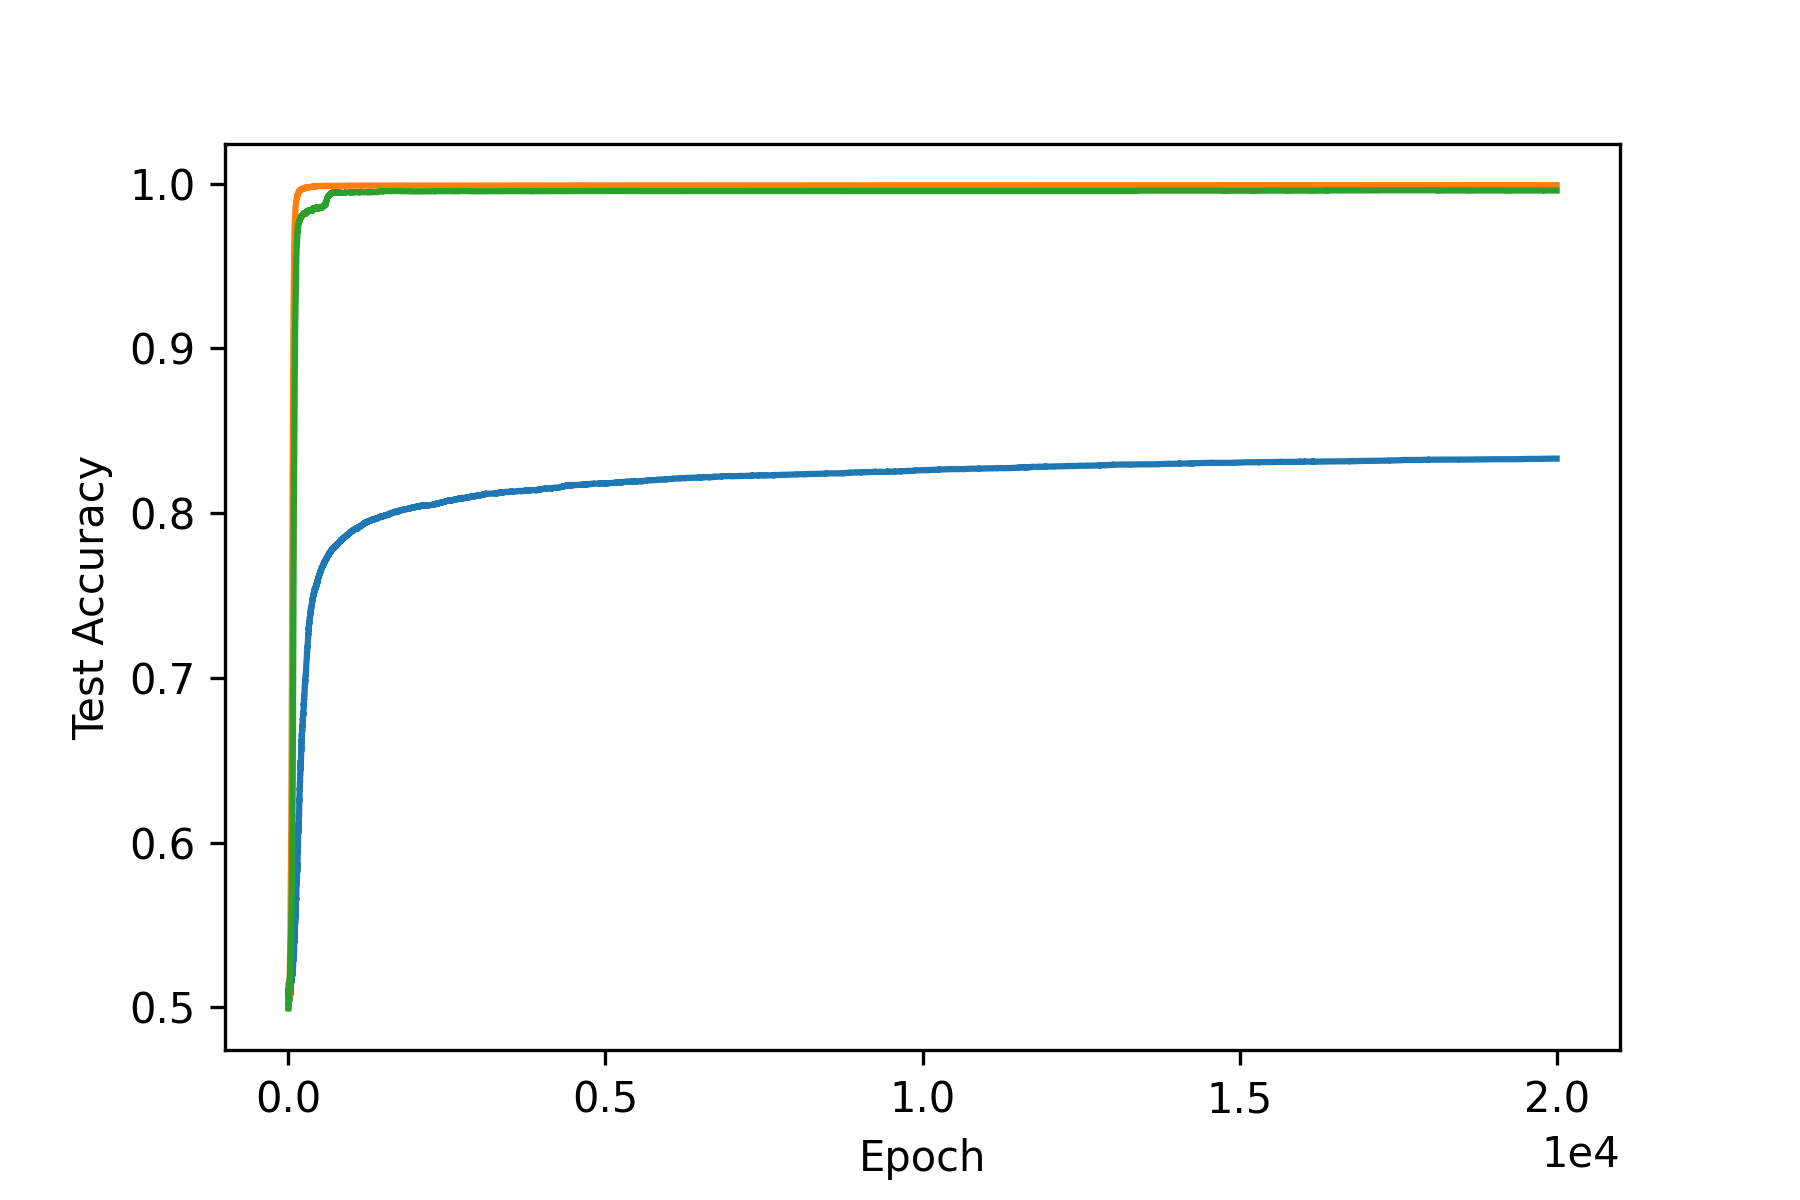
\includegraphics[width=.45\linewidth]{Imgs/Sparse Logistic Regression/test_error_200.png}}\hfill
\subfloat[$N = 100$]{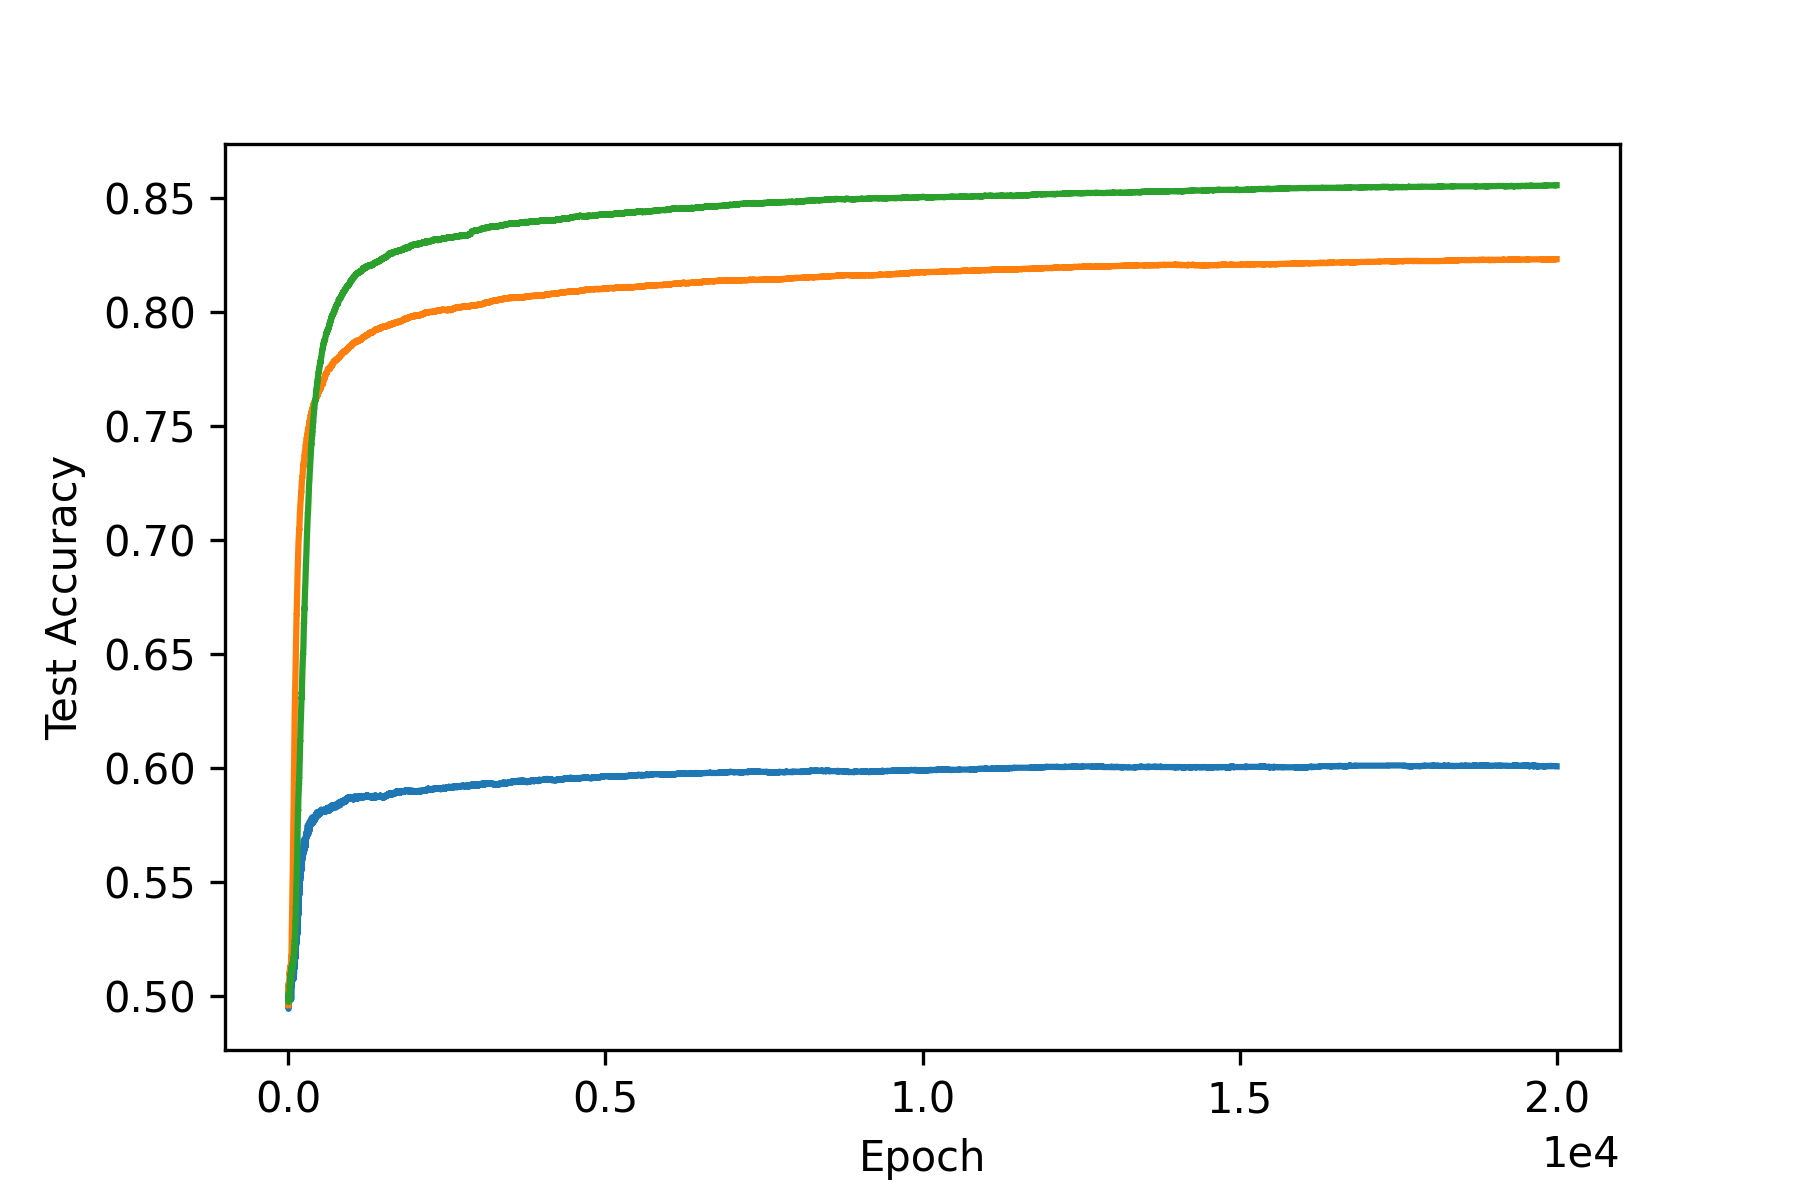
\includegraphics[width=.45\linewidth]{Imgs/Sparse Logistic Regression/test_error_100.png}}\par 
\subfloat[$N = 50$]{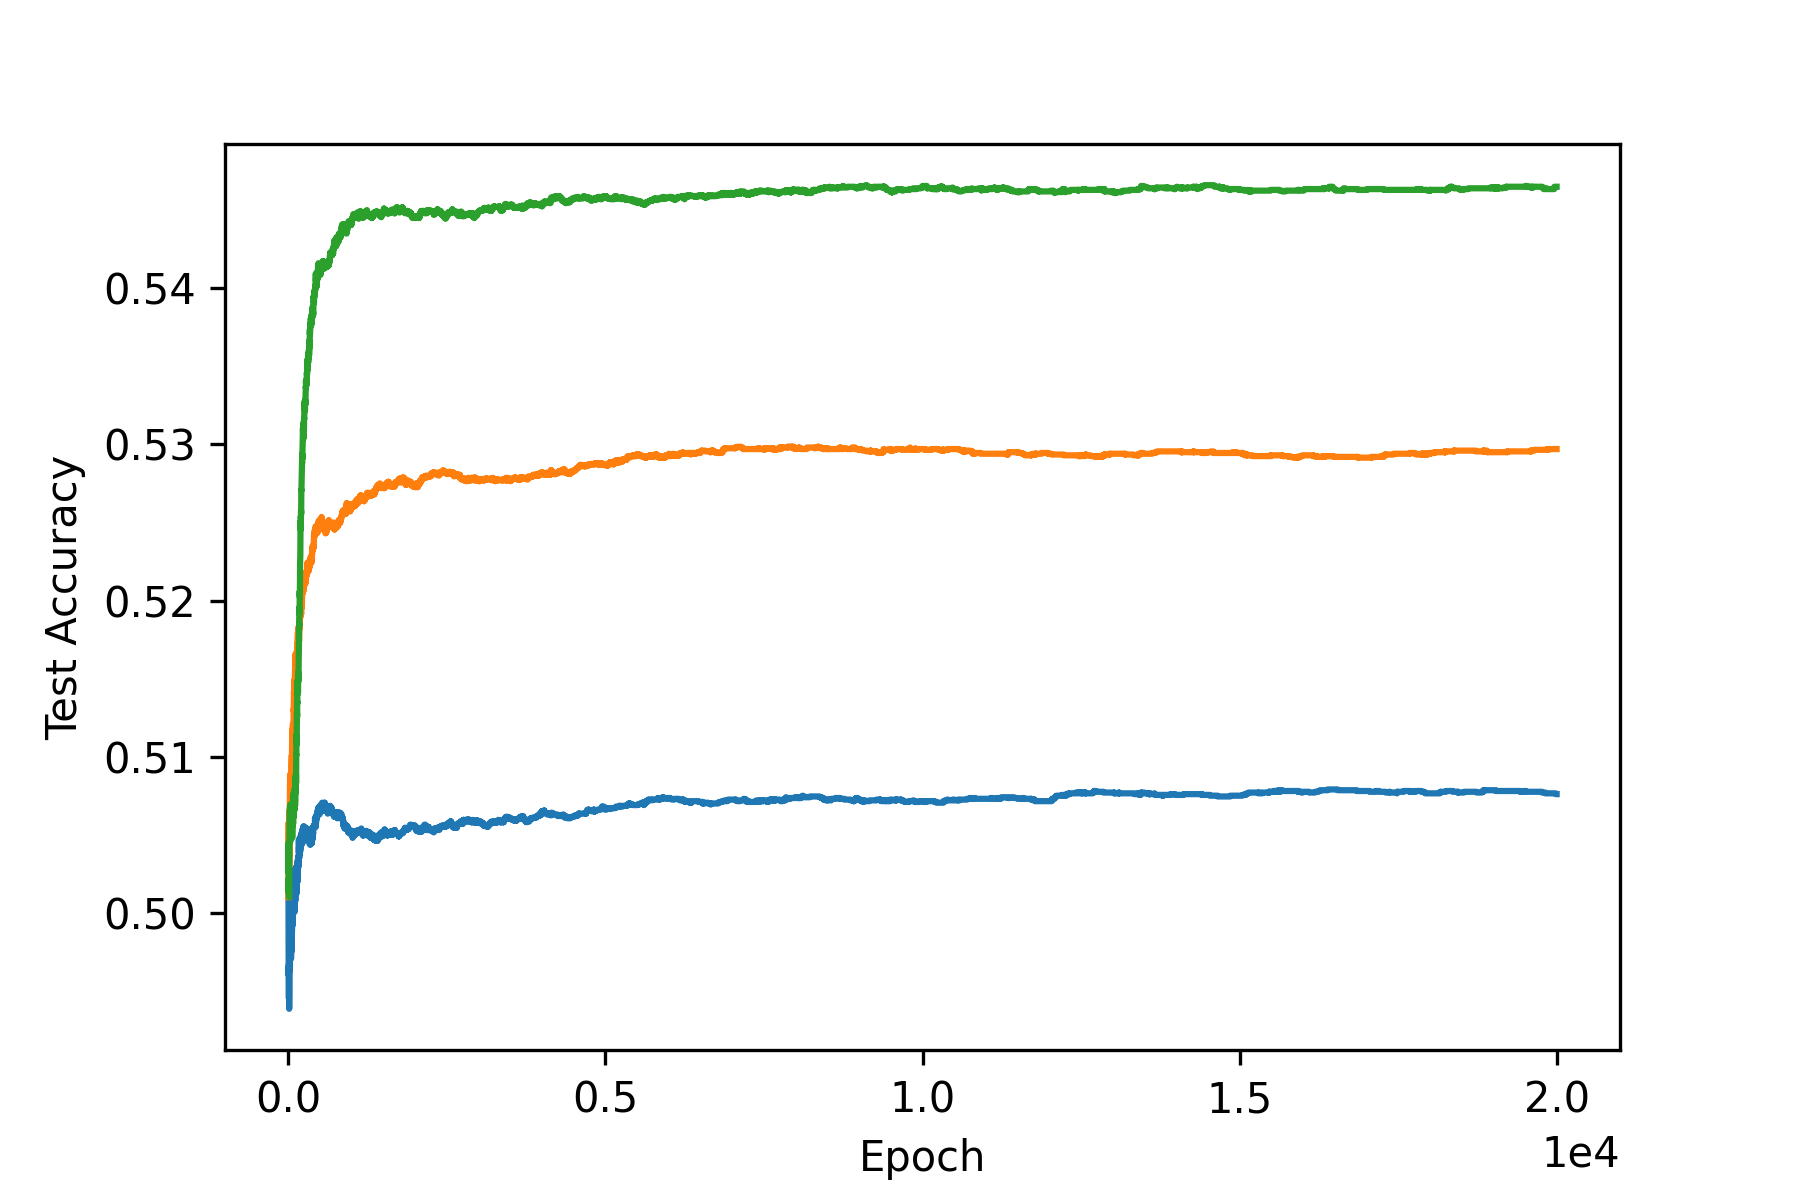
\includegraphics[width=.45\linewidth]{Imgs/Sparse Logistic Regression/test_error_50.png}\label{fig:testerrlogistic50}}
\caption{Average test accuracy versus epoch for $K=20$ gradient descent paths. The test accuracy at epoch $t \in \mathbb{R}_+$ is computed according to $\frac{1}{N_{\text{test}}} \sum_{i=1}^{N_{\text{test}}} \mathbbm{1}_{y_i f\left(\boldsymbol{w}_{r_v, r_{\boldsymbol{u}}}^{(k)}(t), \boldsymbol{x}_i\right) \leq 0}$. The three paths in each plot correspond to the initialization scales $r_w = r_{\boldsymbol{u}} = 1$ (blue), $10^{-1}$ (orange), and $10^{-2}$ (green).}\label{fig:testerrlogistic}
\end{figure}

The results of these experiments, summarized by Figure \ref{fig:testerrlogistic}, provide strong evidence that training for a finite number of epochs with small initialization scale leads to better generalization in the sparse binary classification problem. Precisely, for each of $N \in \{200, 100, 50\}$ we see that the test accuracy averaged over the $K=20$ gradient descent paths is markedly higher throughout the entirety of training for small initialization scale $r_v = r_{\boldsymbol{u}}$. Before any further analysis, we rule out the possibility that these disparities in test error are a result of differences in performance on the training set: each gradient descent path, regardless of the initialization scale $r_v = r_{\boldsymbol{u}}$, interpolates the training data within only 50 to 100 epochs. 

The aforementioned gap in test error is most extreme for $N = 200$: when $r_v = r_{\boldsymbol{u}} \in \{10^{-1}, 10^{-2} \}$, the test accuracy jumps to $1$ almost immediately, whereas when $r_v = r_{\boldsymbol{u}} = 1$ the test accuracy flattens off at around $0.8$. Similarly, for $N=100$ the average test accuracy corresponding to $r_v = r_{\boldsymbol{u}} = 10^{-2}$ is excellent, upwards of $0.85$, whereas that corresponding to $r_v = r_{\boldsymbol{u}} = 1$ is only slightly better than random guessing, around $0.6$. As evidenced by the Figure \ref{fig:testerrlogistic50}, even when the number of training observations $N$ is very small in comparison to the input dimension $n$, we still see gains from initializing the network weights $\boldsymbol{w}$ with small scale $r_v = r_{\boldsymbol{u}}$. 

\begin{figure}[H]
    \centering
    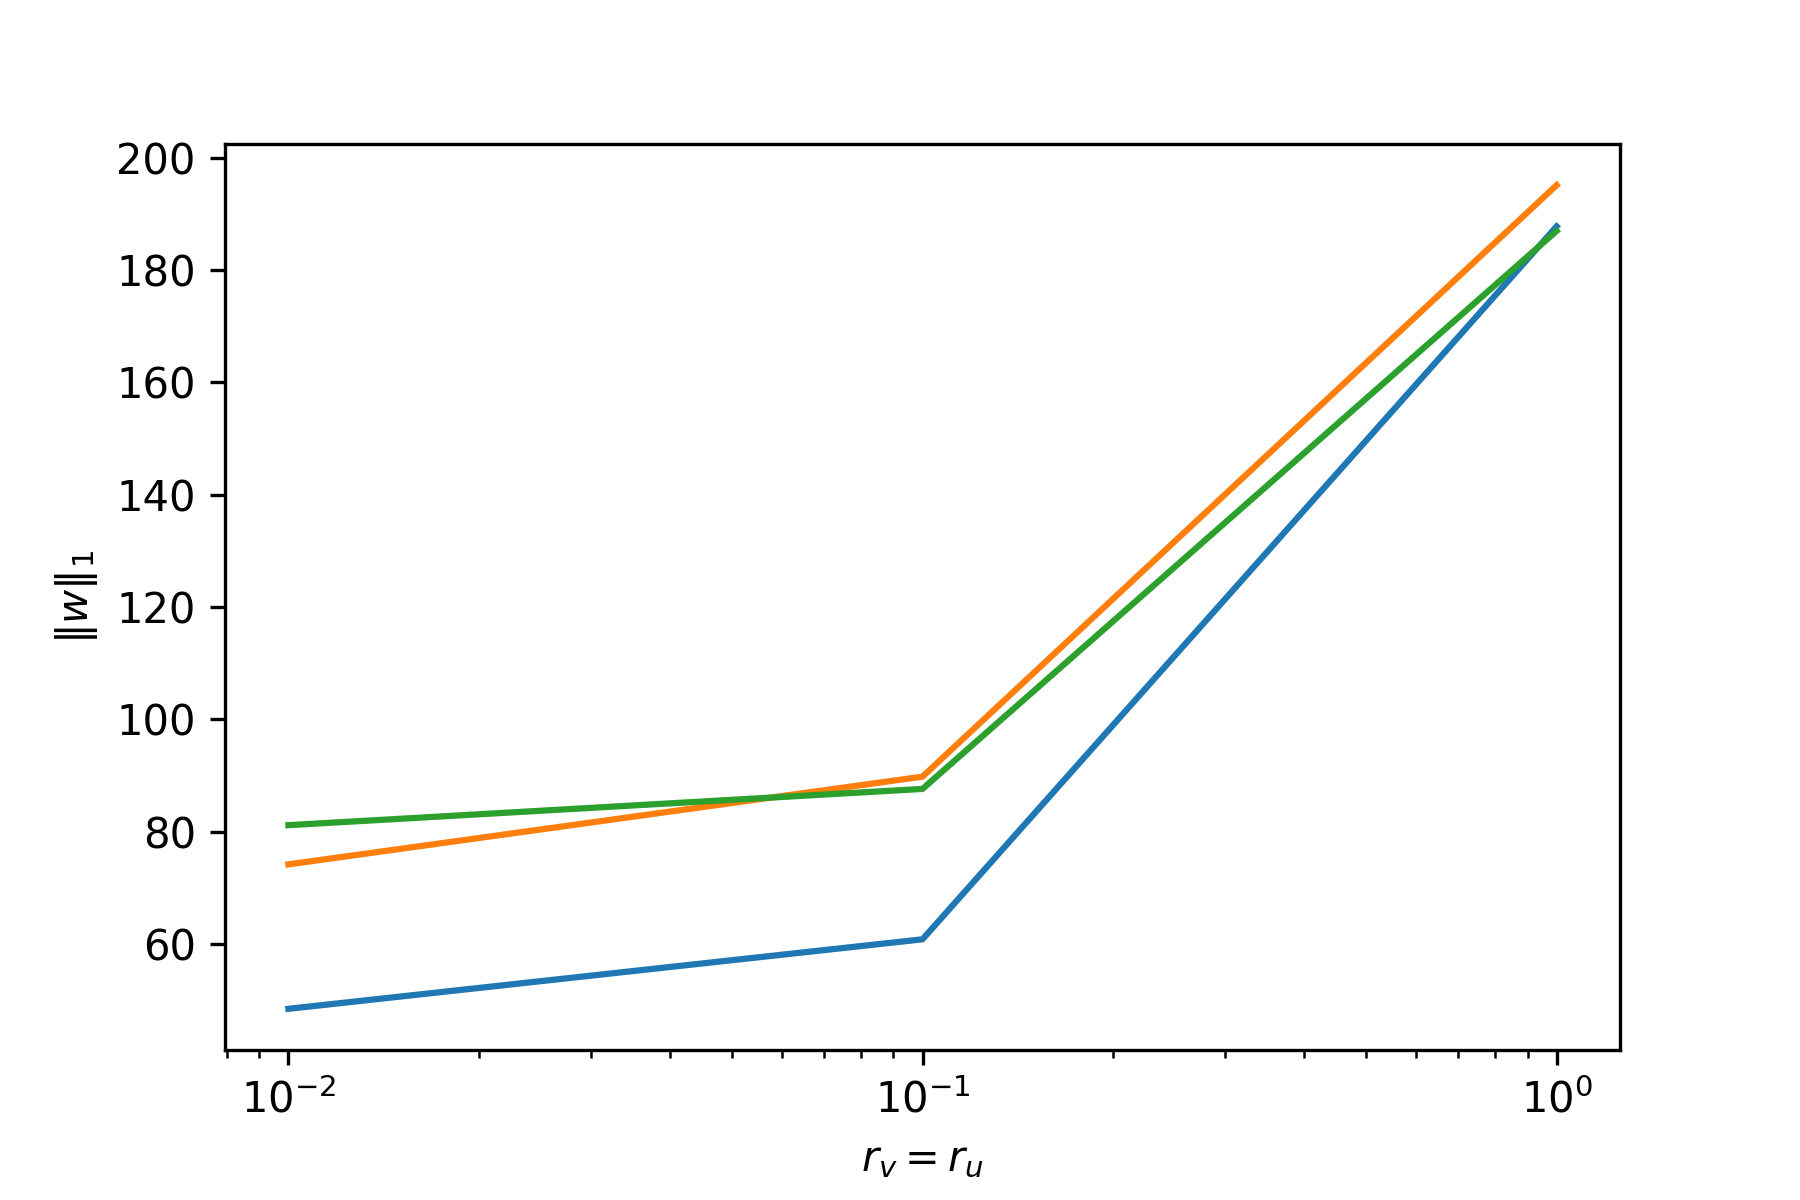
\includegraphics{Imgs/Sparse Logistic Regression/param_l1_avg.png}
    \caption{The average $\ell^1$ norm of the gradient descent path at the end of training, $\boldsymbol{w}_{r_v, r_{\boldsymbol{u}}}(t_{\text{end}})$ for $K=20$ simulations. We include the gradient descent simulations corresponding to $N=200$ (blue), $N=100$ (orange), and $N=50$ training samples.}
    \label{fig:solutionl1logistic}
\end{figure}

In Figure \ref{fig:solutionl1logistic}, we address the question of whether or not there exists implicit $\ell^1$ regularization of the gradient descent solution vector $\boldsymbol{w}_{r_v, r_{\boldsymbol{u}}}(t_{\text{end}})$ in the rich regime. From our previous discussions, we would expect this $\ell^1$ regularization to be most visible in the rich limit $r_v, r_{\boldsymbol{u}} \rightarrow 0$.

Excitingly, for each of $N \in \{200, 100, 50\}$ we discern drastic decreases in the average $\ell^1$ norm of the gradient descent solution $\boldsymbol{w}_{r_v, r_{\boldsymbol{u}}}$ as $r_v = r_{\boldsymbol{u}}$ decreases from $1$ to $10^{-1}$. That is, the neural network solution implemented at the end of gradient descent is much more sparse in its weights for initialization $r_v, r_{\boldsymbol{u}}$ small. We also notice that while there is a sharp decrease in the average $\ell^1$ norm of the gradient descent vector $\boldsymbol{w}_{r_v, r_{\boldsymbol{u}}}(t_{\text{end}})$ when shifting the initialization scale from $r_v = r_{\boldsymbol{u}} = 1$ to $r_v = r_{\boldsymbol{u}} = 10^{-1}$, the decrease is relatively small for the shift from $10^{-1}$ to $10^{-2}$. We suspect that this phenomenon is a consequence of the large stepsize that we previously flagged: since the stepsize $\eta = 10^{-1}$ is so large in comparison to the initialization scales $r_v = r_{\boldsymbol{u}} \in \{10^{-1}, 10^{-2} \}$, the difference between the gradient descent paths corresponding to these two initialization scales is likely almost negligible. Perhaps by performing gradient descent with a smaller stepsize, we would observe a greater distinction between the average $\ell^1$ norm of $\boldsymbol{w}_{r_v, r_{\boldsymbol{u}}}(t_{\text{end}})$ corresponding to $r_v = r_{\boldsymbol{u}} = 10^{-1}$ and $r_v = r_{\boldsymbol{u}} = 10^{-2}$. 

In all, we have provided compelling evidence that training in the rich limit $r_{v}, r_{\boldsymbol{u}} \rightarrow 0$ enforces implicit $\ell^1$ regularization in the gradient descent direction. We believe that this $\ell^1$ regularization is present for all initialization scales, but is not visible when stopping gradient descent at a finite time. This is because, as we discussed in Section \ref{richbinary}, we hypothesize that the gradient flow direction converges more rapidly to its limit when $r_v = r_{\boldsymbol{u}}$ is small. This result is noteworthy, as neither the existing theory of Chizat nor that of Woodworth would suggest this regularization. 

The next step in our investigation of the sparse binary classification problem is to compare the generalization of the implicit $\ell^1$ regularization we have demonstrated in the limit $r_v, r_{\boldsymbol{u}} \rightarrow 0$ with the explicit $\ell^2$ regularization employed by Wei and colleagues \cite{wei2019regularization}. One will recall from Theorem \ref{weithm2.1} that for a neural network with at least four hidden units, training with the $\ell^2$ regularized logistic loss achieves generalization error
\begin{align*}
   \mathbb{P}_{(x,y) \sim \rho}[f(\boldsymbol{w}_{\lambda}, \boldsymbol{x})y \leq 0] \lesssim \sqrt{\frac{n}{N}}.
\end{align*}
But as we previously mentioned, we believe that $\ell^1$ regularization would serve as a better proxy than $\ell^2$ regularization for producing a weight vector $\boldsymbol{w}$ that is $\ell^0$ sparse. Consequently, it is our conjecture that the implicit $\ell^1$ regularization we demonstrated in the rich regime achieves a generalization bound at least as good as, if not better than, that in Theorem \ref{weithm2.1}.

In order to get an approximation of the bound on $\mathbb{P}_{(x,y) \sim \rho, v_i, \boldsymbol{u}_i}[f(\boldsymbol{w}_{r_v, r_{\boldsymbol{u}}}^{\star}, \boldsymbol{x})y \leq 0]$, we must see how the number of training samples necessary to attain population risk less than some threshold $p^{\star}$ changes as a function of the input dimension $n$. For our experiment, we fix $r_{v} = r_{\boldsymbol{u}} = 10^{-1}$ and take $p^{\star} = 0.4$. We choose $r_{v} = r_{\boldsymbol{u}} = 10^{-1}$ because, as we demonstrated in our previous simulations, it seems to be the case that $(\boldsymbol{w}_{r_v = r_{\boldsymbol{u}} = 10^{-1}}(t))_{t \geq 0}$ converges in direction to its rich limit much faster than when $r_{v}, r_{\boldsymbol{u}}$ are small. 

\begin{figure}[H]
\centering
\subfloat[]{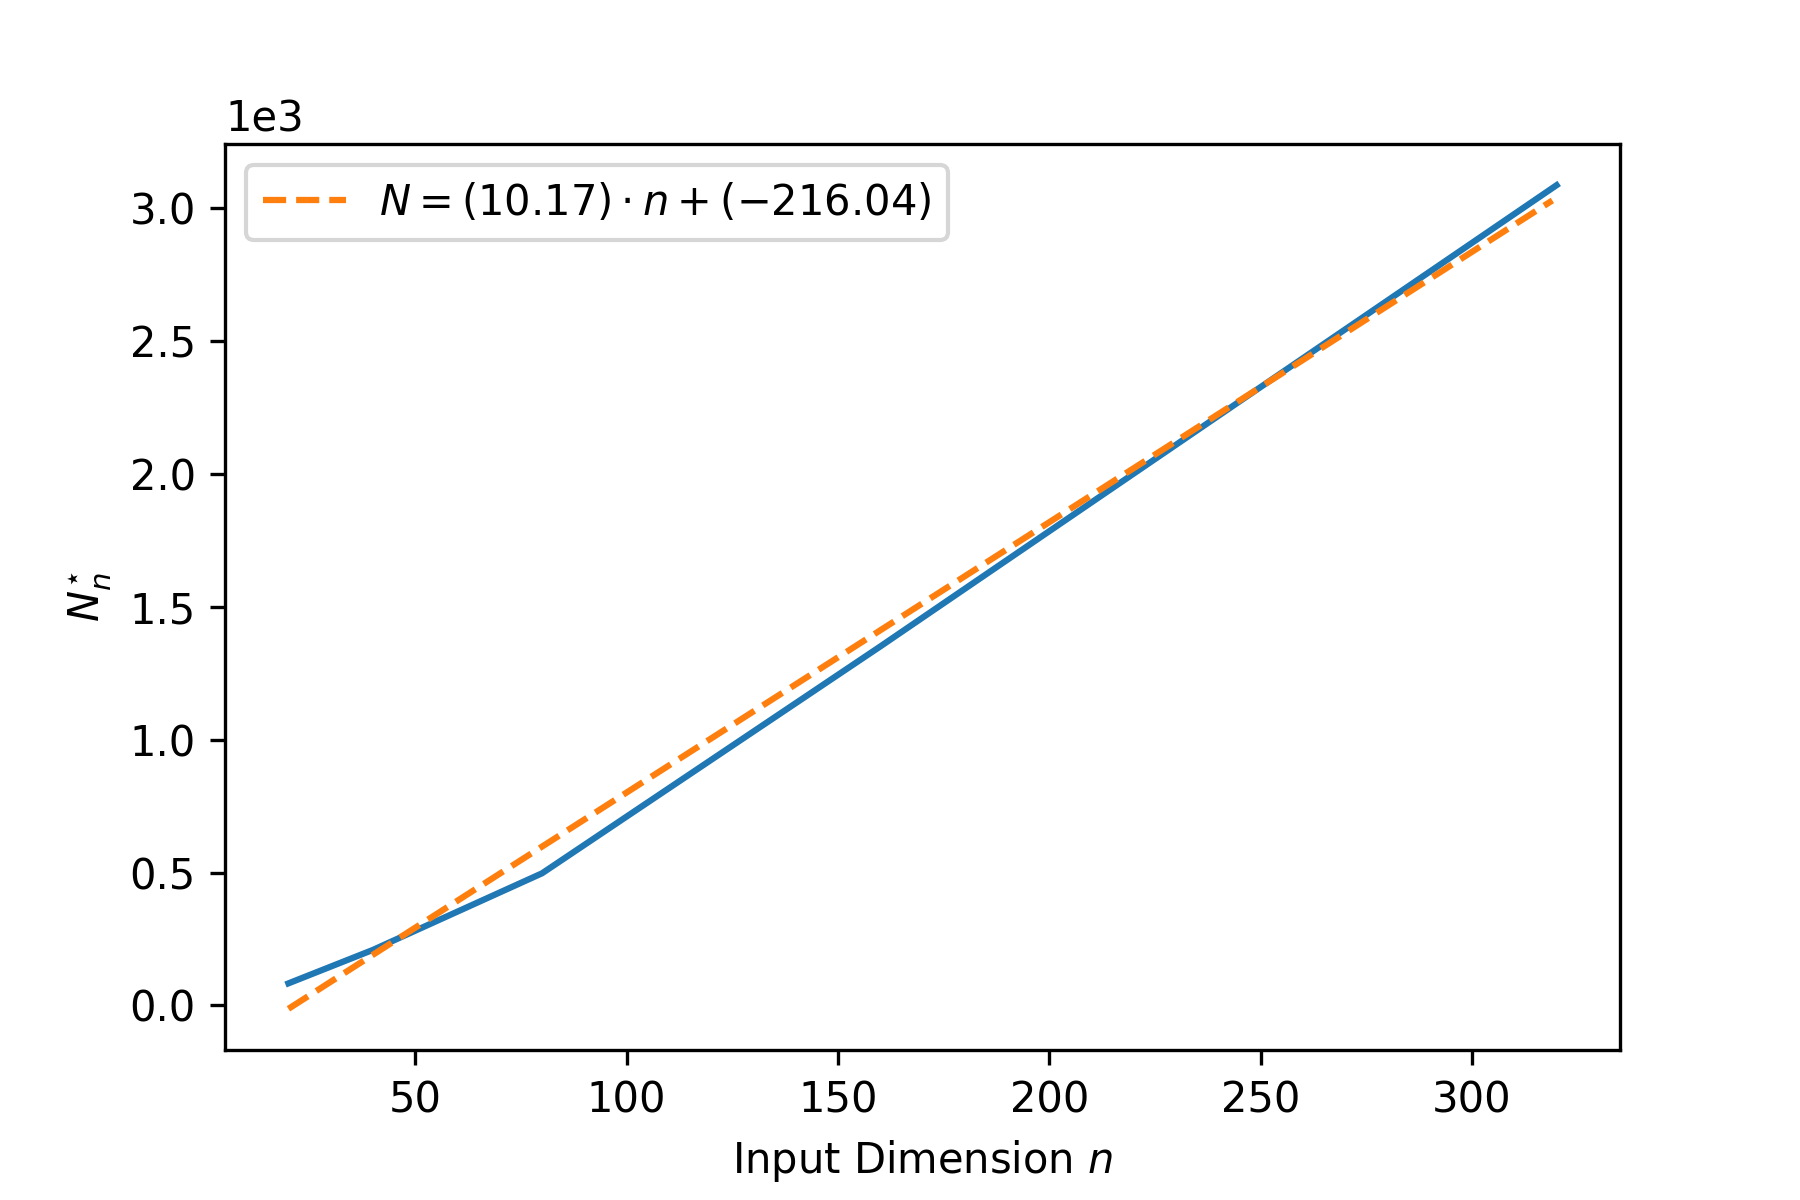
\includegraphics[width=.45\linewidth]{Imgs/Sparse Logistic Regression/min_N_60.png}\label{fig:numsampleslinearfit}}\hfill
\subfloat[]{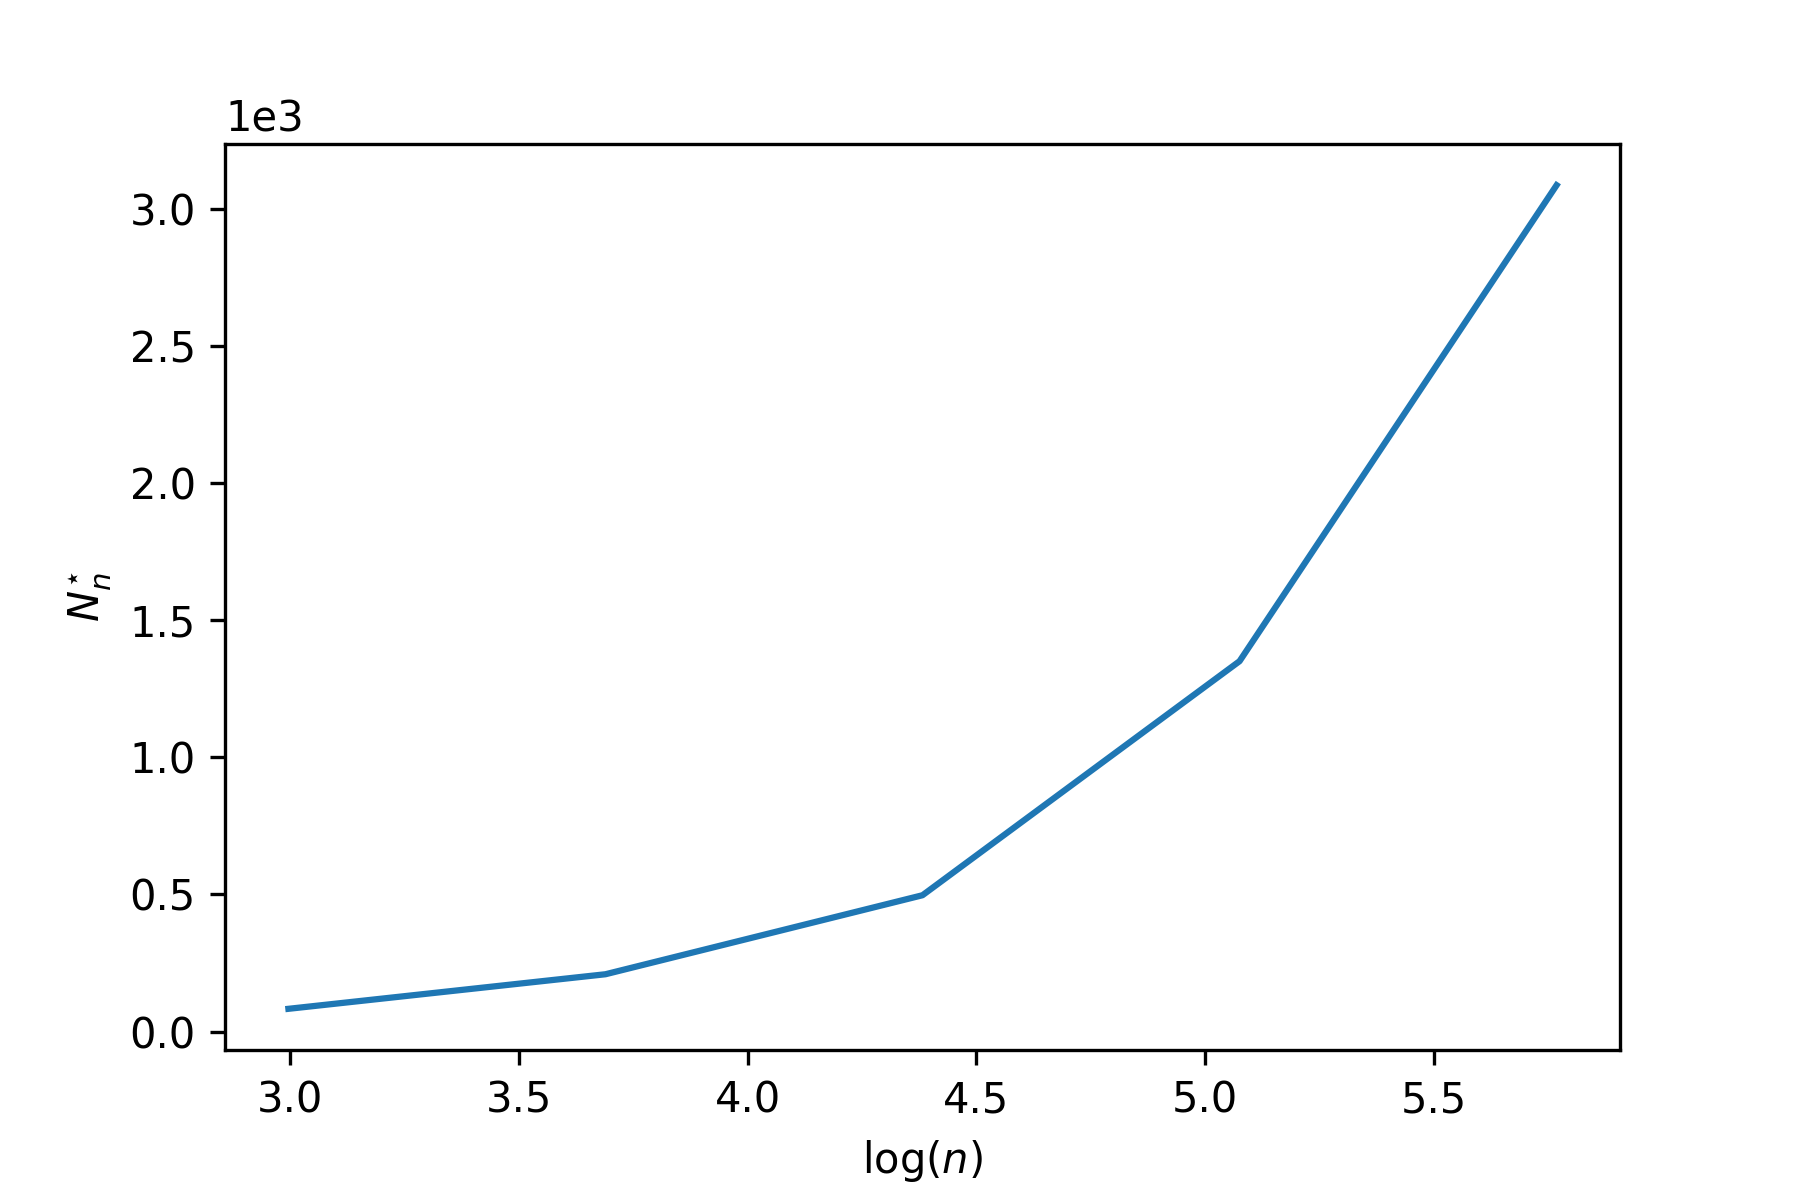
\includegraphics[width=.45\linewidth]{Imgs/Sparse Logistic Regression/min_N_60_log.png}\label{fig:numsampleslog}}
\caption{The minimum number of training samples, $N_n^{\star}$, necessary to attain average test accuracy $\geq 0.6$ with input dimension $n$. $K=10$ gradient descent simulations are used to determined the average test error. (a) We fit a simple linear regression model to estimate the constant $C$ such that $\mathbb{P}_{(\boldsymbol{x}, y) \sim \rho, r_v, r_{\boldsymbol{u}}}[f(\boldsymbol{w}_{r_v, r_{\boldsymbol{u}}}^{\star}, \boldsymbol{x})y \leq 0] \leq \sqrt{\frac{C \cdot d}{n}}$ (b) The input dimension $n$ is replaced with $\log(n)$.}\label{fig:numsamples}
\end{figure}

Just as in the previous set of experiments, we use $\frac{1}{N_{\text{test}}} \sum_{i=1}^{N_{\text{test}}} \mathbbm{1}_{y_i f\left(\boldsymbol{w}_{r_v, r_{\boldsymbol{u}}}^{(k)}(t_{\text{end}}), \boldsymbol{x}_i\right) \leq 0}$ averaged over $K$ gradient descent trials as a proxy for the population risk. And so for each value of the input dimension $n$, we would like to find the smallest number of training samples $N_n^{\star}$ needed to obtain average test accuracy $1-p^{\star}$ averaged over $K$ trials.

Clearly, this is a computationally burdensome experiment: for each input dimension $n$, we must search over values of $N$, performing $K$ gradient descent simulations each time, to find the smallest value which achieves average test accuracy $\geq 1-p^{\star}$. Accordingly, it is necessary that we make modifications to our previous experimental conditions. Specifically, we reduce the total number of training epochs to $10^4$ and the number of gradient trials to $K = 10$. And as for the input dimension, we consider values $n \in \{20, 40, 80, 160, 320\}$. As we will discuss later in our analysis, this is quite a restrictive range of values for $n$.

Despite the limitations of our experiment, the results we obtain are quite compelling. In Figure \ref{fig:numsamples}, we plot the input dimension $n$ against the minimum number of training samples $N_n^{\star}$ necessary to achieve test accuracy $\geq 1-p^{\star} = 0.6$. We observe that there exists an almost perfectly linear relationship between $n$ and $N_n^{\star}$. That is, it appears that a $\Delta n$ increase in the input dimension $n$ corresponds to a $C \cdot \Delta n$ increase in $N_n^{\star}$ for some constant $C \in \mathbb{R}_{++}$. In Figure \ref{fig:numsampleslinearfit}, we obtain an explicit estimate for the value of the slope coefficient $C$ by fitting a linear regression model. The regression model estimates $C \approx 10.17$ and has coefficient of determination $r^2 = 0.996$.

The reason why this linear fit is so interesting is that it suggests the following bound on the population risk of the predictor implemented by the limiting gradient flow direction:
\begin{align*}
   \mathbb{P}_{(x,y) \sim \rho, v_i, \boldsymbol{u}_i}[f(\boldsymbol{w}_{r_v = r_{\boldsymbol{u}} = 10^{-1}}^{\star}, \boldsymbol{x})y \leq 0] \lesssim \sqrt{\frac{n}{N}}, \quad \boldsymbol{w}_{r_v = r_{\boldsymbol{u}} = 10^{-1}}^{\star} = \lim_{t \to \infty} \frac{\boldsymbol{w}_{r_v = r_{\boldsymbol{u}} = 10^{-1}}(t)}{\Vert \boldsymbol{w}_{r_v = r_{\boldsymbol{u}} = 10^{-1}}(t) \Vert_2}.
\end{align*}
That is, we have provided evidence to indicate that the generalization bound we achieve by training in the rich regime is on the same order as that we achieve by adding an explicit $\ell^2$ regularization term to the logistic loss $L$ \cite{wei2019regularization}.\footnote{At the time of writing my thesis, Dr.~Zhou and I were surprised to observe that the generalization error bound achieved in the rich regime appeared to be on the same order as that of the predictor $f(\boldsymbol{w}_{\lambda}, \boldsymbol{x})$ in Theorem \ref{weithm2.1}. However, now that I am knowledgeable about the theory presented by Lyu and Li, this result makes much more sense \cite{lyu2019gradient}. In particular, they prove that the vector to which gradient flow direction converges is proportional to a KKT point of the $\ell^2$ max-margin problem. If the limiting gradient flow direction is, in fact, proportional to a max-margin solution, then we would expect our model to attain a generalization bound similar to that of the predictor resulting from gradient flow on the $\ell^2$ regularized loss. Also, implicit regularization in the parameter space and in the predictor space are completely different. Therefore, although the limit gradient flow direction in the parameter space may be proportional to a $\ell^2$ max-margin direction, the resulting predictor may nonetheless be sparse in the Hilbert space $\mathcal{F}$. To preserve the original state of my paper, I did not alter my analysis, although I have summarized these insights here.} 

Presumably, from the theory of Lyu and Li, we would observe this same generalization bound for larger initialization scales $r_v, r_{\boldsymbol{u}}$ should we train our model sufficiently long. Together, this experiment and the previous make a compelling argument for training with $r_v, r_{\boldsymbol{u}}$ small: although the implicit biases of gradient flow may be the same for all scales in the infinite time limit, they are much more manifest at finite training times when $r_v, r_{\boldsymbol{u}}$ are small. More simply, training with $r_v, r_{\boldsymbol{u}}$ small leads to \enquote{richer} behavior and generalization early-on in training. 

To conclude our discussion, we consider the possibility that the implicit $\ell^1$ regularization present in the rich regime outperforms explicit $\ell^2$ regularization. So far, we have only discussed the possibility that the implicit regularization present in rich training performs just as well as the explicit $\ell^2$ regularization. However, from Figure \ref{fig:solutionl1logistic} it is reasonable to hypothesize that rich training imposes implicit $\ell^1$ regularization on the gradient flow path. If this were true, we might expect to obtain a better generalization bound:
\begin{align*}
   \mathbb{P}_{(x,y) \sim \rho, v_i, \boldsymbol{u}_i}[f(\boldsymbol{w}_{r_v = r_{\boldsymbol{u}} = 10^{-1}}^{\star}, \boldsymbol{x})y \leq 0] \lesssim \sqrt{\frac{\log(n)}{N}}
\end{align*}
than that in Theorem \ref{weithm2.1} resulting from an $\ell^2$ regularizer. While our experimental results do not suggest such a bound, they also do not rule it out either. Expressly, as evidenced by Figure \ref{fig:numsampleslog}, we do not observe a linear relationship between $\log(n)$ and $N_n^{\star}$. This being said, we also comment that the range of values we have for $\log(n)$ is so small that, if such a bound were to exist, it would be difficult to detect in our experimental data anyways. Accordingly, if we wanted to more rigorously consider whether or not a bound of this order exists, we would need to perform the same experiment with much larger $n$.

\section{Conclusion}

As a whole, our work has provided a detailed look at two opposing limits present in neural network training. Recall that we began our paper by formalizing the kernel and rich limits, explaining what they mean in terms of the gradient flow on the scaled objective $\frac{1}{\alpha^2}L(\alpha h(\boldsymbol{w}))$, $(\boldsymbol{w}_{\alpha}(t))_{t \geq 0}$, and under what conditions they are each observed. Following this discussion, we conducted a number of experiments to visualize each of the network function, the neural tangent kernel, and the network weights as gradient flow interpolates between the kernel and rich regimes. The visualizations we produced provide fresh intuition for the kernel and rich limits that is not captured by the theory alone. And for the most exciting portion of our research, we investigated how networks trained near the kernel and rich limits generalize in problems where the underlying distribution of data $\rho$ is sparse. Our experimental results corresponding to the sparse binary classification problem posed by Wei and colleagues are especially intriguing. They suggest that by training in the rich regime, one achieves a generalization bound that is on the same order as that achieved by using an explicit $\ell^2$ regularizer in the loss function $L$. These \enquote{rich} biases are best observed at finite training times when the initialization scale of the gradient flow path is small.

Without a doubt, our experimental results make a strong case for further theoretical study into the rich limit. Having provided evidence to suggest that rich training imposes implicit $\ell^1$ regularization on the limiting gradient flow direction, the next step would be to formalize this observation with a theoretical statement. Similarly, we could prove that the limiting gradient flow direction implemented by rich training does, in fact, achieve a generalization error bound on the same order as the $\ell^2$ regularized model.

\pagebreak
% References

\bibliographystyle{siam}
\bibliography{References/biblio}

\end{document}